\documentclass{report}

%%%%%%%%%%%%%%%%%%%%%%%%%%%%%%%%%
% PACKAGE IMPORTS
%%%%%%%%%%%%%%%%%%%%%%%%%%%%%%%%%


\usepackage[tmargin=2cm,rmargin=1in,lmargin=1in,margin=0.85in,bmargin=2cm,footskip=.2in]{geometry}
\usepackage{amsmath,amsfonts,amsthm,amssymb,mathtools}
\usepackage[varbb]{newpxmath}
\usepackage{xfrac}
\usepackage[makeroom]{cancel}
\usepackage{mathtools}
\usepackage{bookmark}
\usepackage{enumitem}
\usepackage{hyperref,theoremref}
\hypersetup{
	pdftitle={Assignment},
	colorlinks=true, linkcolor=doc!90,
	bookmarksnumbered=true,
	bookmarksopen=true
}
\usepackage[most,many,breakable]{tcolorbox}
\usepackage{xcolor}
\usepackage{varwidth}
\usepackage{varwidth}
\usepackage{etoolbox}
%\usepackage{authblk}
\usepackage{nameref}
\usepackage{multicol,array}
\usepackage{tikz-cd}
\usepackage[ruled,vlined,linesnumbered]{algorithm2e}
\usepackage{comment} % enables the use of multi-line comments (\ifx \fi) 
\usepackage{import}
\usepackage{xifthen}
\usepackage{pdfpages}
\usepackage{transparent}

\newcommand\mycommfont[1]{\footnotesize\ttfamily\textcolor{blue}{#1}}
\SetCommentSty{mycommfont}
\newcommand{\incfig}[1]{%
    \def\svgwidth{\columnwidth}
    \import{./figures/}{#1.pdf_tex}
}

\usepackage{tikzsymbols}
\renewcommand\qedsymbol{$\Laughey$}


%\usepackage{import}
%\usepackage{xifthen}
%\usepackage{pdfpages}
%\usepackage{transparent}


%%%%%%%%%%%%%%%%%%%%%%%%%%%%%%
% SELF MADE COLORS
%%%%%%%%%%%%%%%%%%%%%%%%%%%%%%



\definecolor{myg}{RGB}{56, 140, 70}
\definecolor{myb}{RGB}{45, 111, 177}
\definecolor{myr}{RGB}{199, 68, 64}
\definecolor{mytheorembg}{HTML}{F2F2F9}
\definecolor{mytheoremfr}{HTML}{00007B}
\definecolor{mylenmabg}{HTML}{FFFAF8}
\definecolor{mylenmafr}{HTML}{983b0f}
\definecolor{mypropbg}{HTML}{f2fbfc}
\definecolor{mypropfr}{HTML}{191971}
\definecolor{myexamplebg}{HTML}{F2FBF8}
\definecolor{myexamplefr}{HTML}{88D6D1}
\definecolor{myexampleti}{HTML}{2A7F7F}
\definecolor{mydefinitbg}{HTML}{E5E5FF}
\definecolor{mydefinitfr}{HTML}{3F3FA3}
\definecolor{notesgreen}{RGB}{0,162,0}
\definecolor{myp}{RGB}{197, 92, 212}
\definecolor{mygr}{HTML}{2C3338}
\definecolor{myred}{RGB}{127,0,0}
\definecolor{myyellow}{RGB}{169,121,69}
\definecolor{myexercisebg}{HTML}{F2FBF8}
\definecolor{myexercisefg}{HTML}{88D6D1}


%%%%%%%%%%%%%%%%%%%%%%%%%%%%
% TCOLORBOX SETUPS
%%%%%%%%%%%%%%%%%%%%%%%%%%%%

\setlength{\parindent}{1cm}
%================================
% THEOREM BOX
%================================

\tcbuselibrary{theorems,skins,hooks}
\newtcbtheorem[number within=section]{Theorem}{Theorem}
{%
	enhanced,
	breakable,
	colback = mytheorembg,
	frame hidden,
	boxrule = 0sp,
	borderline west = {2pt}{0pt}{mytheoremfr},
	sharp corners,
	detach title,
	before upper = \tcbtitle\par\smallskip,
	coltitle = mytheoremfr,
	fonttitle = \bfseries\sffamily,
	description font = \mdseries,
	separator sign none,
	segmentation style={solid, mytheoremfr},
}
{th}

\tcbuselibrary{theorems,skins,hooks}
\newtcbtheorem[number within=chapter]{theorem}{Theorem}
{%
	enhanced,
	breakable,
	colback = mytheorembg,
	frame hidden,
	boxrule = 0sp,
	borderline west = {2pt}{0pt}{mytheoremfr},
	sharp corners,
	detach title,
	before upper = \tcbtitle\par\smallskip,
	coltitle = mytheoremfr,
	fonttitle = \bfseries\sffamily,
	description font = \mdseries,
	separator sign none,
	segmentation style={solid, mytheoremfr},
}
{th}


\tcbuselibrary{theorems,skins,hooks}
\newtcolorbox{Theoremcon}
{%
	enhanced
	,breakable
	,colback = mytheorembg
	,frame hidden
	,boxrule = 0sp
	,borderline west = {2pt}{0pt}{mytheoremfr}
	,sharp corners
	,description font = \mdseries
	,separator sign none
}

%================================
% Corollery
%================================
\tcbuselibrary{theorems,skins,hooks}
\newtcbtheorem[number within=section]{Corollary}{Corollary}
{%
	enhanced
	,breakable
	,colback = myp!10
	,frame hidden
	,boxrule = 0sp
	,borderline west = {2pt}{0pt}{myp!85!black}
	,sharp corners
	,detach title
	,before upper = \tcbtitle\par\smallskip
	,coltitle = myp!85!black
	,fonttitle = \bfseries\sffamily
	,description font = \mdseries
	,separator sign none
	,segmentation style={solid, myp!85!black}
}
{th}
\tcbuselibrary{theorems,skins,hooks}
\newtcbtheorem[number within=chapter]{corollary}{Corollary}
{%
	enhanced
	,breakable
	,colback = myp!10
	,frame hidden
	,boxrule = 0sp
	,borderline west = {2pt}{0pt}{myp!85!black}
	,sharp corners
	,detach title
	,before upper = \tcbtitle\par\smallskip
	,coltitle = myp!85!black
	,fonttitle = \bfseries\sffamily
	,description font = \mdseries
	,separator sign none
	,segmentation style={solid, myp!85!black}
}
{th}


%================================
% LENMA
%================================

\tcbuselibrary{theorems,skins,hooks}
\newtcbtheorem[number within=section]{Lenma}{Lenma}
{%
	enhanced,
	breakable,
	colback = mylenmabg,
	frame hidden,
	boxrule = 0sp,
	borderline west = {2pt}{0pt}{mylenmafr},
	sharp corners,
	detach title,
	before upper = \tcbtitle\par\smallskip,
	coltitle = mylenmafr,
	fonttitle = \bfseries\sffamily,
	description font = \mdseries,
	separator sign none,
	segmentation style={solid, mylenmafr},
}
{th}

\tcbuselibrary{theorems,skins,hooks}
\newtcbtheorem[number within=chapter]{lenma}{Lenma}
{%
	enhanced,
	breakable,
	colback = mylenmabg,
	frame hidden,
	boxrule = 0sp,
	borderline west = {2pt}{0pt}{mylenmafr},
	sharp corners,
	detach title,
	before upper = \tcbtitle\par\smallskip,
	coltitle = mylenmafr,
	fonttitle = \bfseries\sffamily,
	description font = \mdseries,
	separator sign none,
	segmentation style={solid, mylenmafr},
}
{th}


%================================
% PROPOSITION
%================================

\tcbuselibrary{theorems,skins,hooks}
\newtcbtheorem[number within=section]{Prop}{Proposition}
{%
	enhanced,
	breakable,
	colback = mypropbg,
	frame hidden,
	boxrule = 0sp,
	borderline west = {2pt}{0pt}{mypropfr},
	sharp corners,
	detach title,
	before upper = \tcbtitle\par\smallskip,
	coltitle = mypropfr,
	fonttitle = \bfseries\sffamily,
	description font = \mdseries,
	separator sign none,
	segmentation style={solid, mypropfr},
}
{th}

\tcbuselibrary{theorems,skins,hooks}
\newtcbtheorem[number within=chapter]{prop}{Proposition}
{%
	enhanced,
	breakable,
	colback = mypropbg,
	frame hidden,
	boxrule = 0sp,
	borderline west = {2pt}{0pt}{mypropfr},
	sharp corners,
	detach title,
	before upper = \tcbtitle\par\smallskip,
	coltitle = mypropfr,
	fonttitle = \bfseries\sffamily,
	description font = \mdseries,
	separator sign none,
	segmentation style={solid, mypropfr},
}
{th}


%================================
% CLAIM
%================================

\tcbuselibrary{theorems,skins,hooks}
\newtcbtheorem[number within=section]{claim}{Claim}
{%
	enhanced
	,breakable
	,colback = myg!10
	,frame hidden
	,boxrule = 0sp
	,borderline west = {2pt}{0pt}{myg}
	,sharp corners
	,detach title
	,before upper = \tcbtitle\par\smallskip
	,coltitle = myg!85!black
	,fonttitle = \bfseries\sffamily
	,description font = \mdseries
	,separator sign none
	,segmentation style={solid, myg!85!black}
}
{th}



%================================
% Exercise
%================================

\tcbuselibrary{theorems,skins,hooks}
\newtcbtheorem[number within=section]{Exercise}{Exercise}
{%
	enhanced,
	breakable,
	colback = myexercisebg,
	frame hidden,
	boxrule = 0sp,
	borderline west = {2pt}{0pt}{myexercisefg},
	sharp corners,
	detach title,
	before upper = \tcbtitle\par\smallskip,
	coltitle = myexercisefg,
	fonttitle = \bfseries\sffamily,
	description font = \mdseries,
	separator sign none,
	segmentation style={solid, myexercisefg},
}
{th}

\tcbuselibrary{theorems,skins,hooks}
\newtcbtheorem[number within=chapter]{exercise}{Exercise}
{%
	enhanced,
	breakable,
	colback = myexercisebg,
	frame hidden,
	boxrule = 0sp,
	borderline west = {2pt}{0pt}{myexercisefg},
	sharp corners,
	detach title,
	before upper = \tcbtitle\par\smallskip,
	coltitle = myexercisefg,
	fonttitle = \bfseries\sffamily,
	description font = \mdseries,
	separator sign none,
	segmentation style={solid, myexercisefg},
}
{th}

%================================
% EXAMPLE BOX
%================================

\newtcbtheorem[number within=section]{Example}{Example}
{%
	colback = myexamplebg
	,breakable
	,colframe = myexamplefr
	,coltitle = myexampleti
	,boxrule = 1pt
	,sharp corners
	,detach title
	,before upper=\tcbtitle\par\smallskip
	,fonttitle = \bfseries
	,description font = \mdseries
	,separator sign none
	,description delimiters parenthesis
}
{ex}

\newtcbtheorem[number within=chapter]{example}{Example}
{%
	colback = myexamplebg
	,breakable
	,colframe = myexamplefr
	,coltitle = myexampleti
	,boxrule = 1pt
	,sharp corners
	,detach title
	,before upper=\tcbtitle\par\smallskip
	,fonttitle = \bfseries
	,description font = \mdseries
	,separator sign none
	,description delimiters parenthesis
}
{ex}

%================================
% DEFINITION BOX
%================================

\newtcbtheorem[number within=section]{Definition}{Definition}{enhanced,
	before skip=2mm,after skip=2mm, colback=red!5,colframe=red!80!black,boxrule=0.5mm,
	attach boxed title to top left={xshift=1cm,yshift*=1mm-\tcboxedtitleheight}, varwidth boxed title*=-3cm,
	boxed title style={frame code={
					\path[fill=tcbcolback]
					([yshift=-1mm,xshift=-1mm]frame.north west)
					arc[start angle=0,end angle=180,radius=1mm]
					([yshift=-1mm,xshift=1mm]frame.north east)
					arc[start angle=180,end angle=0,radius=1mm];
					\path[left color=tcbcolback!60!black,right color=tcbcolback!60!black,
						middle color=tcbcolback!80!black]
					([xshift=-2mm]frame.north west) -- ([xshift=2mm]frame.north east)
					[rounded corners=1mm]-- ([xshift=1mm,yshift=-1mm]frame.north east)
					-- (frame.south east) -- (frame.south west)
					-- ([xshift=-1mm,yshift=-1mm]frame.north west)
					[sharp corners]-- cycle;
				},interior engine=empty,
		},
	fonttitle=\bfseries,
	title={#2},#1}{def}
\newtcbtheorem[number within=chapter]{definition}{Definition}{enhanced,
	before skip=2mm,after skip=2mm, colback=red!5,colframe=red!80!black,boxrule=0.5mm,
	attach boxed title to top left={xshift=1cm,yshift*=1mm-\tcboxedtitleheight}, varwidth boxed title*=-3cm,
	boxed title style={frame code={
					\path[fill=tcbcolback]
					([yshift=-1mm,xshift=-1mm]frame.north west)
					arc[start angle=0,end angle=180,radius=1mm]
					([yshift=-1mm,xshift=1mm]frame.north east)
					arc[start angle=180,end angle=0,radius=1mm];
					\path[left color=tcbcolback!60!black,right color=tcbcolback!60!black,
						middle color=tcbcolback!80!black]
					([xshift=-2mm]frame.north west) -- ([xshift=2mm]frame.north east)
					[rounded corners=1mm]-- ([xshift=1mm,yshift=-1mm]frame.north east)
					-- (frame.south east) -- (frame.south west)
					-- ([xshift=-1mm,yshift=-1mm]frame.north west)
					[sharp corners]-- cycle;
				},interior engine=empty,
		},
	fonttitle=\bfseries,
	title={#2},#1}{def}



%================================
% Solution BOX
%================================

\makeatletter
\newtcbtheorem{question}{Question}{enhanced,
	breakable,
	colback=white,
	colframe=myb!80!black,
	attach boxed title to top left={yshift*=-\tcboxedtitleheight},
	fonttitle=\bfseries,
	title={#2},
	boxed title size=title,
	boxed title style={%
			sharp corners,
			rounded corners=northwest,
			colback=tcbcolframe,
			boxrule=0pt,
		},
	underlay boxed title={%
			\path[fill=tcbcolframe] (title.south west)--(title.south east)
			to[out=0, in=180] ([xshift=5mm]title.east)--
			(title.center-|frame.east)
			[rounded corners=\kvtcb@arc] |-
			(frame.north) -| cycle;
		},
	#1
}{def}
\makeatother

%================================
% SOLUTION BOX
%================================

\makeatletter
\newtcolorbox{solution}{enhanced,
	breakable,
	colback=white,
	colframe=myg!80!black,
	attach boxed title to top left={yshift*=-\tcboxedtitleheight},
	title=Solution,
	boxed title size=title,
	boxed title style={%
			sharp corners,
			rounded corners=northwest,
			colback=tcbcolframe,
			boxrule=0pt,
		},
	underlay boxed title={%
			\path[fill=tcbcolframe] (title.south west)--(title.south east)
			to[out=0, in=180] ([xshift=5mm]title.east)--
			(title.center-|frame.east)
			[rounded corners=\kvtcb@arc] |-
			(frame.north) -| cycle;
		},
}
\makeatother

%================================
% Question BOX
%================================

\makeatletter
\newtcbtheorem{qstion}{Question}{enhanced,
	breakable,
	colback=white,
	colframe=mygr,
	attach boxed title to top left={yshift*=-\tcboxedtitleheight},
	fonttitle=\bfseries,
	title={#2},
	boxed title size=title,
	boxed title style={%
			sharp corners,
			rounded corners=northwest,
			colback=tcbcolframe,
			boxrule=0pt,
		},
	underlay boxed title={%
			\path[fill=tcbcolframe] (title.south west)--(title.south east)
			to[out=0, in=180] ([xshift=5mm]title.east)--
			(title.center-|frame.east)
			[rounded corners=\kvtcb@arc] |-
			(frame.north) -| cycle;
		},
	#1
}{def}
\makeatother

\newtcbtheorem[number within=chapter]{wconc}{Wrong Concept}{
	breakable,
	enhanced,
	colback=white,
	colframe=myr,
	arc=0pt,
	outer arc=0pt,
	fonttitle=\bfseries\sffamily\large,
	colbacktitle=myr,
	attach boxed title to top left={},
	boxed title style={
			enhanced,
			skin=enhancedfirst jigsaw,
			arc=3pt,
			bottom=0pt,
			interior style={fill=myr}
		},
	#1
}{def}



%================================
% NOTE BOX
%================================

\usetikzlibrary{arrows,calc,shadows.blur}
\tcbuselibrary{skins}
\newtcolorbox{note}[1][]{%
	enhanced jigsaw,
	colback=gray!20!white,%
	colframe=gray!80!black,
	size=small,
	boxrule=1pt,
	title=\textbf{Note:},
	halign title=flush center,
	coltitle=black,
	breakable,
	drop shadow=black!50!white,
	attach boxed title to top left={xshift=1cm,yshift=-\tcboxedtitleheight/2,yshifttext=-\tcboxedtitleheight/2},
	minipage boxed title=1.5cm,
	boxed title style={%
			colback=white,
			size=fbox,
			boxrule=1pt,
			boxsep=2pt,
			underlay={%
					\coordinate (dotA) at ($(interior.west) + (-0.5pt,0)$);
					\coordinate (dotB) at ($(interior.east) + (0.5pt,0)$);
					\begin{scope}
						\clip (interior.north west) rectangle ([xshift=3ex]interior.east);
						\filldraw [white, blur shadow={shadow opacity=60, shadow yshift=-.75ex}, rounded corners=2pt] (interior.north west) rectangle (interior.south east);
					\end{scope}
					\begin{scope}[gray!80!black]
						\fill (dotA) circle (2pt);
						\fill (dotB) circle (2pt);
					\end{scope}
				},
		},
	#1,
}

%%%%%%%%%%%%%%%%%%%%%%%%%%%%%%
% SELF MADE COMMANDS
%%%%%%%%%%%%%%%%%%%%%%%%%%%%%%


\newcommand{\thm}[2]{\begin{Theorem}{#1}{}#2\end{Theorem}}
\newcommand{\cor}[2]{\begin{Corollary}{#1}{}#2\end{Corollary}}
\newcommand{\mlenma}[2]{\begin{Lenma}{#1}{}#2\end{Lenma}}
\newcommand{\mprop}[2]{\begin{Prop}{#1}{}#2\end{Prop}}
\newcommand{\clm}[3]{\begin{claim}{#1}{#2}#3\end{claim}}
\newcommand{\wc}[2]{\begin{wconc}{#1}{}\setlength{\parindent}{1cm}#2\end{wconc}}
\newcommand{\thmcon}[1]{\begin{Theoremcon}{#1}\end{Theoremcon}}
\newcommand{\ex}[2]{\begin{Example}{#1}{}#2\end{Example}}
\newcommand{\dfn}[2]{\begin{Definition}[colbacktitle=red!75!black]{#1}{}#2\end{Definition}}
\newcommand{\dfnc}[2]{\begin{definition}[colbacktitle=red!75!black]{#1}{}#2\end{definition}}
\newcommand{\qs}[2]{\begin{question}{#1}{}#2\end{question}}
\newcommand{\pf}[2]{\begin{myproof}[#1]#2\end{myproof}}
\newcommand{\nt}[1]{\begin{note}#1\end{note}}

\newcommand*\circled[1]{\tikz[baseline=(char.base)]{
		\node[shape=circle,draw,inner sep=1pt] (char) {#1};}}
\newcommand\getcurrentref[1]{%
	\ifnumequal{\value{#1}}{0}
	{??}
	{\the\value{#1}}%
}
\newcommand{\getCurrentSectionNumber}{\getcurrentref{section}}
\newenvironment{myproof}[1][\proofname]{%
	\proof[\bfseries #1: ]%
}{\endproof}

\newcommand{\mclm}[2]{\begin{myclaim}[#1]#2\end{myclaim}}
\newenvironment{myclaim}[1][\claimname]{\proof[\bfseries #1: ]}{}

\newcounter{mylabelcounter}

\makeatletter
\newcommand{\setword}[2]{%
	\phantomsection
	#1\def\@currentlabel{\unexpanded{#1}}\label{#2}%
}
\makeatother




\tikzset{
	symbol/.style={
			draw=none,
			every to/.append style={
					edge node={node [sloped, allow upside down, auto=false]{$#1$}}}
		}
}


% deliminators
\DeclarePairedDelimiter{\abs}{\lvert}{\rvert}
\DeclarePairedDelimiter{\norm}{\lVert}{\rVert}

\DeclarePairedDelimiter{\ceil}{\lceil}{\rceil}
\DeclarePairedDelimiter{\floor}{\lfloor}{\rfloor}
\DeclarePairedDelimiter{\round}{\lfloor}{\rceil}

\newsavebox\diffdbox
\newcommand{\slantedromand}{{\mathpalette\makesl{d}}}
\newcommand{\makesl}[2]{%
\begingroup
\sbox{\diffdbox}{$\mathsurround=0pt#1\mathrm{#2}$}%
\pdfsave
\pdfsetmatrix{1 0 0.2 1}%
\rlap{\usebox{\diffdbox}}%
\pdfrestore
\hskip\wd\diffdbox
\endgroup
}
\newcommand{\dd}[1][]{\ensuremath{\mathop{}\!\ifstrempty{#1}{%
\slantedromand\@ifnextchar^{\hspace{0.2ex}}{\hspace{0.1ex}}}%
{\slantedromand\hspace{0.2ex}^{#1}}}}
\ProvideDocumentCommand\dv{o m g}{%
  \ensuremath{%
    \IfValueTF{#3}{%
      \IfNoValueTF{#1}{%
        \frac{\dd #2}{\dd #3}%
      }{%
        \frac{\dd^{#1} #2}{\dd #3^{#1}}%
      }%
    }{%
      \IfNoValueTF{#1}{%
        \frac{\dd}{\dd #2}%
      }{%
        \frac{\dd^{#1}}{\dd #2^{#1}}%
      }%
    }%
  }%
}
\providecommand*{\pdv}[3][]{\frac{\partial^{#1}#2}{\partial#3^{#1}}}
%  - others
\DeclareMathOperator{\Lap}{\mathcal{L}}
\DeclareMathOperator{\Var}{Var} % varience
\DeclareMathOperator{\Cov}{Cov} % covarience
\DeclareMathOperator{\E}{E} % expected

% Since the amsthm package isn't loaded

% I prefer the slanted \leq
\let\oldleq\leq % save them in case they're every wanted
\let\oldgeq\geq
\renewcommand{\leq}{\leqslant}
\renewcommand{\geq}{\geqslant}

% % redefine matrix env to allow for alignment, use r as default
% \renewcommand*\env@matrix[1][r]{\hskip -\arraycolsep
%     \let\@ifnextchar\new@ifnextchar
%     \array{*\c@MaxMatrixCols #1}}


%\usepackage{framed}
%\usepackage{titletoc}
%\usepackage{etoolbox}
%\usepackage{lmodern}


%\patchcmd{\tableofcontents}{\contentsname}{\sffamily\contentsname}{}{}

%\renewenvironment{leftbar}
%{\def\FrameCommand{\hspace{6em}%
%		{\color{myyellow}\vrule width 2pt depth 6pt}\hspace{1em}}%
%	\MakeFramed{\parshape 1 0cm \dimexpr\textwidth-6em\relax\FrameRestore}\vskip2pt%
%}
%{\endMakeFramed}

%\titlecontents{chapter}
%[0em]{\vspace*{2\baselineskip}}
%{\parbox{4.5em}{%
%		\hfill\Huge\sffamily\bfseries\color{myred}\thecontentspage}%
%	\vspace*{-2.3\baselineskip}\leftbar\textsc{\small\chaptername~\thecontentslabel}\\\sffamily}
%{}{\endleftbar}
%\titlecontents{section}
%[8.4em]
%{\sffamily\contentslabel{3em}}{}{}
%{\hspace{0.5em}\nobreak\itshape\color{myred}\contentspage}
%\titlecontents{subsection}
%[8.4em]
%{\sffamily\contentslabel{3em}}{}{}  
%{\hspace{0.5em}\nobreak\itshape\color{myred}\contentspage}



%%%%%%%%%%%%%%%%%%%%%%%%%%%%%%%%%%%%%%%%%%%
% TABLE OF CONTENTS
%%%%%%%%%%%%%%%%%%%%%%%%%%%%%%%%%%%%%%%%%%%

\usepackage{tikz}
\definecolor{doc}{RGB}{0,60,110}
\usepackage{titletoc}
\contentsmargin{0cm}
\titlecontents{chapter}[3.7pc]
{\addvspace{30pt}%
	\begin{tikzpicture}[remember picture, overlay]%
		\draw[fill=doc!60,draw=doc!60] (-7,-.1) rectangle (-0.9,.5);%
		\pgftext[left,x=-3.5cm,y=0.2cm]{\color{white}\Large\sc\bfseries Chapter\ \thecontentslabel};%
	\end{tikzpicture}\color{doc!60}\large\sc\bfseries}%
{}
{}
{\;\titlerule\;\large\sc\bfseries Page \thecontentspage
	\begin{tikzpicture}[remember picture, overlay]
		\draw[fill=doc!60,draw=doc!60] (2pt,0) rectangle (4,0.1pt);
	\end{tikzpicture}}%
\titlecontents{section}[3.7pc]
{\addvspace{2pt}}
{\contentslabel[\thecontentslabel]{2pc}}
{}
{\hfill\small \thecontentspage}
[]
\titlecontents*{subsection}[3.7pc]
{\addvspace{-1pt}\small}
{}
{}
{\ --- \small\thecontentspage}
[ \textbullet\ ][]

\makeatletter
\renewcommand{\tableofcontents}{%
	\chapter*{%
	  \vspace*{-20\p@}%
	  \begin{tikzpicture}[remember picture, overlay]%
		  \pgftext[right,x=15cm,y=0.2cm]{\color{doc!60}\Huge\sc\bfseries \contentsname};%
		  \draw[fill=doc!60,draw=doc!60] (13,-.75) rectangle (20,1);%
		  \clip (13,-.75) rectangle (20,1);
		  \pgftext[right,x=15cm,y=0.2cm]{\color{white}\Huge\sc\bfseries \contentsname};%
	  \end{tikzpicture}}%
	\@starttoc{toc}}
\makeatother


% My commands %
\newcommand{\innerproduct}[2]{\langle #1, #2 \rangle}
\newcommand{\generators}[1]{\langle #1 \rangle}

%From M275 "Topology" at SJSU
\newcommand{\id}{\mathrm{id}}
\newcommand{\taking}[1]{\xrightarrow{#1}}
\newcommand{\inv}{^{-1}}

%From M170 "Introduction to Graph Theory" at SJSU
\DeclareMathOperator{\diam}{diam}
\DeclareMathOperator{\ord}{ord}
\newcommand{\defeq}{\overset{\mathrm{def}}{=}}

%From the USAMO .tex files
\newcommand{\ts}{\textsuperscript}
\newcommand{\dg}{^\circ}
\newcommand{\ii}{\item}

% % From Math 55 and Math 145 at Harvard
% \newenvironment{subproof}[1][Proof]{%
% \begin{proof}[#1] \renewcommand{\qedsymbol}{$\blacksquare$}}%
% {\end{proof}}

\newcommand{\liff}{\leftrightarrow}
\newcommand{\lthen}{\rightarrow}
\newcommand{\opname}{\operatorname}
\newcommand{\surjto}{\twoheadrightarrow}
\newcommand{\injto}{\hookrightarrow}
\newcommand{\On}{\mathrm{On}} % ordinals
\DeclareMathOperator{\img}{im} % Image
\DeclareMathOperator{\Img}{Im} % Image
\DeclareMathOperator{\coker}{coker} % Cokernel
\DeclareMathOperator{\Coker}{Coker} % Cokernel
\DeclareMathOperator{\Ker}{Ker} % Kernel
\DeclareMathOperator{\rank}{rank}
\DeclareMathOperator{\Spec}{Spec} % spectrum
\DeclareMathOperator{\Tr}{Tr} % trace
\DeclareMathOperator{\pr}{pr} % projection
\DeclareMathOperator{\ext}{ext} % extension
\DeclareMathOperator{\pred}{pred} % predecessor
\DeclareMathOperator{\dom}{dom} % domain
\DeclareMathOperator{\ran}{ran} % range
\DeclareMathOperator{\Hom}{Hom} % homomorphism
\DeclareMathOperator{\Mor}{Mor} % morphisms
\DeclareMathOperator{\End}{End} % endomorphism

\newcommand{\eps}{\epsilon}
\newcommand{\veps}{\varepsilon}
\newcommand{\ol}{\overline}
\newcommand{\ul}{\underline}
\newcommand{\wt}{\widetilde}
\newcommand{\wh}{\widehat}
\newcommand{\vocab}[1]{\textbf{\color{blue} #1}}
\providecommand{\half}{\frac{1}{2}}
\newcommand{\dang}{\measuredangle} %% Directed angle
\newcommand{\ray}[1]{\overrightarrow{#1}}
\newcommand{\seg}[1]{\overline{#1}}
\newcommand{\arc}[1]{\wideparen{#1}}
\DeclareMathOperator{\cis}{cis}
\DeclareMathOperator*{\lcm}{lcm}
\DeclareMathOperator*{\argmin}{arg min}
\DeclareMathOperator*{\argmax}{arg max}
\newcommand{\cycsum}{\sum_{\mathrm{cyc}}}
\newcommand{\symsum}{\sum_{\mathrm{sym}}}
\newcommand{\cycprod}{\prod_{\mathrm{cyc}}}
\newcommand{\symprod}{\prod_{\mathrm{sym}}}
\newcommand{\Qed}{\begin{flushright}\qed\end{flushright}}
\newcommand{\parinn}{\setlength{\parindent}{1cm}}
\newcommand{\parinf}{\setlength{\parindent}{0cm}}
% \newcommand{\norm}{\|\cdot\|}
\newcommand{\inorm}{\norm_{\infty}}
\newcommand{\opensets}{\{V_{\alpha}\}_{\alpha\in I}}
\newcommand{\oset}{V_{\alpha}}
\newcommand{\opset}[1]{V_{\alpha_{#1}}}
\newcommand{\lub}{\text{lub}}
\newcommand{\del}[2]{\frac{\partial #1}{\partial #2}}
\newcommand{\Del}[3]{\frac{\partial^{#1} #2}{\partial^{#1} #3}}
\newcommand{\deld}[2]{\dfrac{\partial #1}{\partial #2}}
\newcommand{\Deld}[3]{\dfrac{\partial^{#1} #2}{\partial^{#1} #3}}
\newcommand{\lm}{\lambda}
\newcommand{\uin}{\mathbin{\rotatebox[origin=c]{90}{$\in$}}}
\newcommand{\usubset}{\mathbin{\rotatebox[origin=c]{90}{$\subset$}}}
\newcommand{\lt}{\left}
\newcommand{\rt}{\right}
\newcommand{\bs}[1]{\boldsymbol{#1}}
\newcommand{\exs}{\exists}
\newcommand{\st}{\strut}
\newcommand{\dps}[1]{\displaystyle{#1}}

\newcommand{\sol}{\setlength{\parindent}{0cm}\textbf{\textit{Solution:}}\setlength{\parindent}{1cm} }
\newcommand{\solve}[1]{\setlength{\parindent}{0cm}\textbf{\textit{Solution: }}\setlength{\parindent}{1cm}#1 \Qed}

% Things Lie
\newcommand{\kb}{\mathfrak b}
\newcommand{\kg}{\mathfrak g}
\newcommand{\kh}{\mathfrak h}
\newcommand{\kn}{\mathfrak n}
\newcommand{\ku}{\mathfrak u}
\newcommand{\kz}{\mathfrak z}
\DeclareMathOperator{\Ext}{Ext} % Ext functor
\DeclareMathOperator{\Tor}{Tor} % Tor functor
\newcommand{\gl}{\opname{\mathfrak{gl}}} % frak gl group
\renewcommand{\sl}{\opname{\mathfrak{sl}}} % frak sl group chktex 6

% More script letters etc.
\newcommand{\SA}{\mathcal A}
\newcommand{\SB}{\mathcal B}
\newcommand{\SC}{\mathcal C}
\newcommand{\SF}{\mathcal F}
\newcommand{\SG}{\mathcal G}
\newcommand{\SH}{\mathcal H}
\newcommand{\OO}{\mathcal O}

\newcommand{\SCA}{\mathscr A}
\newcommand{\SCB}{\mathscr B}
\newcommand{\SCC}{\mathscr C}
\newcommand{\SCD}{\mathscr D}
\newcommand{\SCE}{\mathscr E}
\newcommand{\SCF}{\mathscr F}
\newcommand{\SCG}{\mathscr G}
\newcommand{\SCH}{\mathscr H}

% Mathfrak primes
\newcommand{\km}{\mathfrak m}
\newcommand{\kp}{\mathfrak p}
\newcommand{\kq}{\mathfrak q}

% number sets
\newcommand{\RR}[1][]{\ensuremath{\ifstrempty{#1}{\mathbb{R}}{\mathbb{R}^{#1}}}}
\newcommand{\NN}[1][]{\ensuremath{\ifstrempty{#1}{\mathbb{N}}{\mathbb{N}^{#1}}}}
\newcommand{\ZZ}[1][]{\ensuremath{\ifstrempty{#1}{\mathbb{Z}}{\mathbb{Z}^{#1}}}}
\newcommand{\QQ}[1][]{\ensuremath{\ifstrempty{#1}{\mathbb{Q}}{\mathbb{Q}^{#1}}}}
\newcommand{\CC}[1][]{\ensuremath{\ifstrempty{#1}{\mathbb{C}}{\mathbb{C}^{#1}}}}
\newcommand{\PP}[1][]{\ensuremath{\ifstrempty{#1}{\mathbb{P}}{\mathbb{P}^{#1}}}}
\newcommand{\HH}[1][]{\ensuremath{\ifstrempty{#1}{\mathbb{H}}{\mathbb{H}^{#1}}}}
\newcommand{\FF}[1][]{\ensuremath{\ifstrempty{#1}{\mathbb{F}}{\mathbb{F}^{#1}}}}
% expected value
\newcommand{\EE}{\ensuremath{\mathbb{E}}}
\newcommand{\charin}{\text{ char }}
\DeclareMathOperator{\sign}{sign}
\DeclareMathOperator{\Aut}{Aut}
\DeclareMathOperator{\Inn}{Inn}
\DeclareMathOperator{\Syl}{Syl}
\DeclareMathOperator{\Gal}{Gal}
\DeclareMathOperator{\GL}{GL} % General linear group
\DeclareMathOperator{\SL}{SL} % Special linear group

%---------------------------------------
% BlackBoard Math Fonts :-
%---------------------------------------

%Captital Letters
\newcommand{\bbA}{\mathbb{A}}	\newcommand{\bbB}{\mathbb{B}}
\newcommand{\bbC}{\mathbb{C}}	\newcommand{\bbD}{\mathbb{D}}
\newcommand{\bbE}{\mathbb{E}}	\newcommand{\bbF}{\mathbb{F}}
\newcommand{\bbG}{\mathbb{G}}	\newcommand{\bbH}{\mathbb{H}}
\newcommand{\bbI}{\mathbb{I}}	\newcommand{\bbJ}{\mathbb{J}}
\newcommand{\bbK}{\mathbb{K}}	\newcommand{\bbL}{\mathbb{L}}
\newcommand{\bbM}{\mathbb{M}}	\newcommand{\bbN}{\mathbb{N}}
\newcommand{\bbO}{\mathbb{O}}	\newcommand{\bbP}{\mathbb{P}}
\newcommand{\bbQ}{\mathbb{Q}}	\newcommand{\bbR}{\mathbb{R}}
\newcommand{\bbS}{\mathbb{S}}	\newcommand{\bbT}{\mathbb{T}}
\newcommand{\bbU}{\mathbb{U}}	\newcommand{\bbV}{\mathbb{V}}
\newcommand{\bbW}{\mathbb{W}}	\newcommand{\bbX}{\mathbb{X}}
\newcommand{\bbY}{\mathbb{Y}}	\newcommand{\bbZ}{\mathbb{Z}}

%---------------------------------------
% MathCal Fonts :-
%---------------------------------------

%Captital Letters
\newcommand{\mcA}{\mathcal{A}}	\newcommand{\mcB}{\mathcal{B}}
\newcommand{\mcC}{\mathcal{C}}	\newcommand{\mcD}{\mathcal{D}}
\newcommand{\mcE}{\mathcal{E}}	\newcommand{\mcF}{\mathcal{F}}
\newcommand{\mcG}{\mathcal{G}}	\newcommand{\mcH}{\mathcal{H}}
\newcommand{\mcI}{\mathcal{I}}	\newcommand{\mcJ}{\mathcal{J}}
\newcommand{\mcK}{\mathcal{K}}	\newcommand{\mcL}{\mathcal{L}}
\newcommand{\mcM}{\mathcal{M}}	\newcommand{\mcN}{\mathcal{N}}
\newcommand{\mcO}{\mathcal{O}}	\newcommand{\mcP}{\mathcal{P}}
\newcommand{\mcQ}{\mathcal{Q}}	\newcommand{\mcR}{\mathcal{R}}
\newcommand{\mcS}{\mathcal{S}}	\newcommand{\mcT}{\mathcal{T}}
\newcommand{\mcU}{\mathcal{U}}	\newcommand{\mcV}{\mathcal{V}}
\newcommand{\mcW}{\mathcal{W}}	\newcommand{\mcX}{\mathcal{X}}
\newcommand{\mcY}{\mathcal{Y}}	\newcommand{\mcZ}{\mathcal{Z}}


%---------------------------------------
% Bold Math Fonts :-
%---------------------------------------

%Captital Letters
\newcommand{\bmA}{\boldsymbol{A}}	\newcommand{\bmB}{\boldsymbol{B}}
\newcommand{\bmC}{\boldsymbol{C}}	\newcommand{\bmD}{\boldsymbol{D}}
\newcommand{\bmE}{\boldsymbol{E}}	\newcommand{\bmF}{\boldsymbol{F}}
\newcommand{\bmG}{\boldsymbol{G}}	\newcommand{\bmH}{\boldsymbol{H}}
\newcommand{\bmI}{\boldsymbol{I}}	\newcommand{\bmJ}{\boldsymbol{J}}
\newcommand{\bmK}{\boldsymbol{K}}	\newcommand{\bmL}{\boldsymbol{L}}
\newcommand{\bmM}{\boldsymbol{M}}	\newcommand{\bmN}{\boldsymbol{N}}
\newcommand{\bmO}{\boldsymbol{O}}	\newcommand{\bmP}{\boldsymbol{P}}
\newcommand{\bmQ}{\boldsymbol{Q}}	\newcommand{\bmR}{\boldsymbol{R}}
\newcommand{\bmS}{\boldsymbol{S}}	\newcommand{\bmT}{\boldsymbol{T}}
\newcommand{\bmU}{\boldsymbol{U}}	\newcommand{\bmV}{\boldsymbol{V}}
\newcommand{\bmW}{\boldsymbol{W}}	\newcommand{\bmX}{\boldsymbol{X}}
\newcommand{\bmY}{\boldsymbol{Y}}	\newcommand{\bmZ}{\boldsymbol{Z}}
%Small Letters
\newcommand{\bma}{\boldsymbol{a}}	\newcommand{\bmb}{\boldsymbol{b}}
\newcommand{\bmc}{\boldsymbol{c}}	\newcommand{\bmd}{\boldsymbol{d}}
\newcommand{\bme}{\boldsymbol{e}}	\newcommand{\bmf}{\boldsymbol{f}}
\newcommand{\bmg}{\boldsymbol{g}}	\newcommand{\bmh}{\boldsymbol{h}}
\newcommand{\bmi}{\boldsymbol{i}}	\newcommand{\bmj}{\boldsymbol{j}}
\newcommand{\bmk}{\boldsymbol{k}}	\newcommand{\bml}{\boldsymbol{l}}
\newcommand{\bmm}{\boldsymbol{m}}	\newcommand{\bmn}{\boldsymbol{n}}
\newcommand{\bmo}{\boldsymbol{o}}	\newcommand{\bmp}{\boldsymbol{p}}
\newcommand{\bmq}{\boldsymbol{q}}	\newcommand{\bmr}{\boldsymbol{r}}
\newcommand{\bms}{\boldsymbol{s}}	\newcommand{\bmt}{\boldsymbol{t}}
\newcommand{\bmu}{\boldsymbol{u}}	\newcommand{\bmv}{\boldsymbol{v}}
\newcommand{\bmw}{\boldsymbol{w}}	\newcommand{\bmx}{\boldsymbol{x}}
\newcommand{\bmy}{\boldsymbol{y}}	\newcommand{\bmz}{\boldsymbol{z}}

%---------------------------------------
% Scr Math Fonts :-
%---------------------------------------

\newcommand{\sA}{{\mathscr{A}}}   \newcommand{\sB}{{\mathscr{B}}}
\newcommand{\sC}{{\mathscr{C}}}   \newcommand{\sD}{{\mathscr{D}}}
\newcommand{\sE}{{\mathscr{E}}}   \newcommand{\sF}{{\mathscr{F}}}
\newcommand{\sG}{{\mathscr{G}}}   \newcommand{\sH}{{\mathscr{H}}}
\newcommand{\sI}{{\mathscr{I}}}   \newcommand{\sJ}{{\mathscr{J}}}
\newcommand{\sK}{{\mathscr{K}}}   \newcommand{\sL}{{\mathscr{L}}}
\newcommand{\sM}{{\mathscr{M}}}   \newcommand{\sN}{{\mathscr{N}}}
\newcommand{\sO}{{\mathscr{O}}}   \newcommand{\sP}{{\mathscr{P}}}
\newcommand{\sQ}{{\mathscr{Q}}}   \newcommand{\sR}{{\mathscr{R}}}
\newcommand{\sS}{{\mathscr{S}}}   \newcommand{\sT}{{\mathscr{T}}}
\newcommand{\sU}{{\mathscr{U}}}   \newcommand{\sV}{{\mathscr{V}}}
\newcommand{\sW}{{\mathscr{W}}}   \newcommand{\sX}{{\mathscr{X}}}
\newcommand{\sY}{{\mathscr{Y}}}   \newcommand{\sZ}{{\mathscr{Z}}}


%---------------------------------------
% Math Fraktur Font
%---------------------------------------

%Captital Letters
\newcommand{\mfA}{\mathfrak{A}}	\newcommand{\mfB}{\mathfrak{B}}
\newcommand{\mfC}{\mathfrak{C}}	\newcommand{\mfD}{\mathfrak{D}}
\newcommand{\mfE}{\mathfrak{E}}	\newcommand{\mfF}{\mathfrak{F}}
\newcommand{\mfG}{\mathfrak{G}}	\newcommand{\mfH}{\mathfrak{H}}
\newcommand{\mfI}{\mathfrak{I}}	\newcommand{\mfJ}{\mathfrak{J}}
\newcommand{\mfK}{\mathfrak{K}}	\newcommand{\mfL}{\mathfrak{L}}
\newcommand{\mfM}{\mathfrak{M}}	\newcommand{\mfN}{\mathfrak{N}}
\newcommand{\mfO}{\mathfrak{O}}	\newcommand{\mfP}{\mathfrak{P}}
\newcommand{\mfQ}{\mathfrak{Q}}	\newcommand{\mfR}{\mathfrak{R}}
\newcommand{\mfS}{\mathfrak{S}}	\newcommand{\mfT}{\mathfrak{T}}
\newcommand{\mfU}{\mathfrak{U}}	\newcommand{\mfV}{\mathfrak{V}}
\newcommand{\mfW}{\mathfrak{W}}	\newcommand{\mfX}{\mathfrak{X}}
\newcommand{\mfY}{\mathfrak{Y}}	\newcommand{\mfZ}{\mathfrak{Z}}
%Small Letters
\newcommand{\mfa}{\mathfrak{a}}	\newcommand{\mfb}{\mathfrak{b}}
\newcommand{\mfc}{\mathfrak{c}}	\newcommand{\mfd}{\mathfrak{d}}
\newcommand{\mfe}{\mathfrak{e}}	\newcommand{\mff}{\mathfrak{f}}
\newcommand{\mfg}{\mathfrak{g}}	\newcommand{\mfh}{\mathfrak{h}}
\newcommand{\mfi}{\mathfrak{i}}	\newcommand{\mfj}{\mathfrak{j}}
\newcommand{\mfk}{\mathfrak{k}}	\newcommand{\mfl}{\mathfrak{l}}
\newcommand{\mfm}{\mathfrak{m}}	\newcommand{\mfn}{\mathfrak{n}}
\newcommand{\mfo}{\mathfrak{o}}	\newcommand{\mfp}{\mathfrak{p}}
\newcommand{\mfq}{\mathfrak{q}}	\newcommand{\mfr}{\mathfrak{r}}
\newcommand{\mfs}{\mathfrak{s}}	\newcommand{\mft}{\mathfrak{t}}
\newcommand{\mfu}{\mathfrak{u}}	\newcommand{\mfv}{\mathfrak{v}}
\newcommand{\mfw}{\mathfrak{w}}	\newcommand{\mfx}{\mathfrak{x}}
\newcommand{\mfy}{\mathfrak{y}}	\newcommand{\mfz}{\mathfrak{z}}

\usepackage{xcolor}
\usepackage{tikz-qtree}
\usepackage{graphicx}



\newcommand{
    \red
    }[1]{
        \textcolor{red}{#1}
        }
        \newcommand{\esempio}[1]{
            \ex{}{#1}
}
\newcommand{\teorema}[1]{\thm{}{#1}}
\newcommand{\dimostrazione}[1]{\pf{Dimostrazione}{#1}}
\setlength{\parindent}{0pt}
\newcommand{\osservazione}[1]{\nt{#1}}

\title{\Huge{Linguaggi di programmazione}\\Appunti}
\author{\huge{GioLaPalma}}
\date{}
\pagenumbering{gobble}

\graphicspath{{paginette/img/}}

\begin{document}

\maketitle
\newpage% or \cleardoublepage
% \pdfbookmark[<level>]{<title>}{<dest>}
\pdfbookmark[section]{\contentsname}{toc}

\tableofcontents

\pagebreak

\chapter{Introduzione ai linguaggi normali: grammatiche}


\section{Linguaggi (naturali o artificiali)}

La descrizione di un linguaggio avviene su 3 dimensioni:
\begin{itemize}
    \item \textbf{Sintassi}: regole di formazione, ovvero la relazione tra segni
    \item \textbf{Semantica}: attribuzione di significato
    \item \textbf{Pregmatica}: in quale modo frasi corrette e sensate sono usate
    \item \textbf{Implementazione}: come eseguire una frase corretta rispettandone la semantica
\end{itemize}

Partiamo con il descrivere questi elementi

\subsection{Sintassi}

\dfn{sintassi}{La \textbf{sintassi} è la parte della grammatica che studia la struttura delle frasi e il modo in cui le parole si combinano per formare enunciati corretti e significativi}


Si dirama in diversi aspetti: 
\begin{itemize}
    \item \textbf{Aspetto lessicale} che riguarda le parole che si possono usare, quindi:
    \begin{itemize}
        \item descrizione del lessico, intuitivamente i dizionari per i linguaggi naturali assolvono a questo compito
        \item errori dovuti a vocaboli inesistenti
    \end{itemize}
    \item \textbf{Aspetto grammaticale} che si riferisce nel modo in cui è possibile costruire frasi corrette è possibile cotruire con il lessico. Le frasi grammaticalmente corrette possono essere costruite grazie all'uso delle regole grammaticali, che sono in numero finito, mentre il numero di frasi generabili è infinito.
    
    Un errore grammaticale è una frase scorretta, anche se il lessico utilizzato è corretto. Es. "La cane abbaiano"
\end{itemize}

\subsection{Semantica}
\dfn{Semantica}{La \textbf{semantica} è la branca della linguistica che studia il significato delle parole, delle frasi e degli enunciati}

\begin{itemize}
    \item \red{Per il lessico} (quindi lo studio e il significato delle parole) bastano \red{i dizionari}
    \item \red{Per le frasi} è più complicato, \red{devo sapere} infatti:
    \begin{enumerate}
        \item a \red{quale linguaggio appartiene la frase}
        \item su \red{quale linguaggio basarmi per dare significato}
    \end{enumerate}
\end{itemize}

\begin{center}

    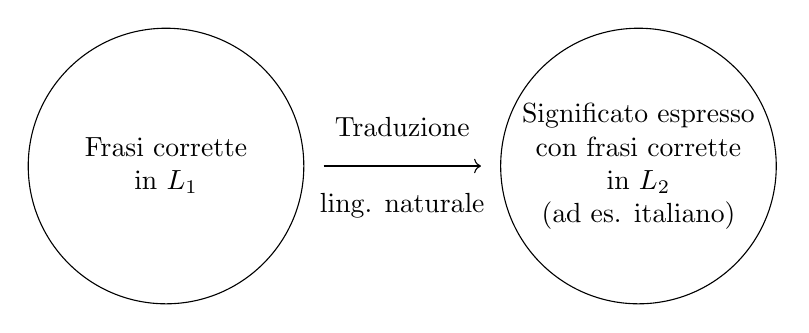
\begin{tikzpicture}
        % Primo cerchio (Frasi corrette in L1)
        \draw (0,0) circle (1.75cm);
        \node at (0,0) {\begin{tabular}{c}
                         Frasi corrette \\ 
                         in \textit{$L_1$}
                         \end{tabular}};
                         
        % Secondo cerchio (Significato espresso con frasi corrette in L2)
        \draw (6,0) circle (1.75cm);
        \node at (6,0) {\begin{tabular}{c}
                         Significato espresso \\ 
                         con frasi corrette \\ 
                         in \textit{$L_2$} \\ 
                         (ad es. italiano)
                         \end{tabular}};
        
        % Freccia tra i due cerchi
        \draw[->] (2,0) -- (4,0);
        \node at (3,0.5) {Traduzione};
        \node at (3,-0.5) {ling. naturale};
    \end{tikzpicture}
\end{center}
\begin{center}
    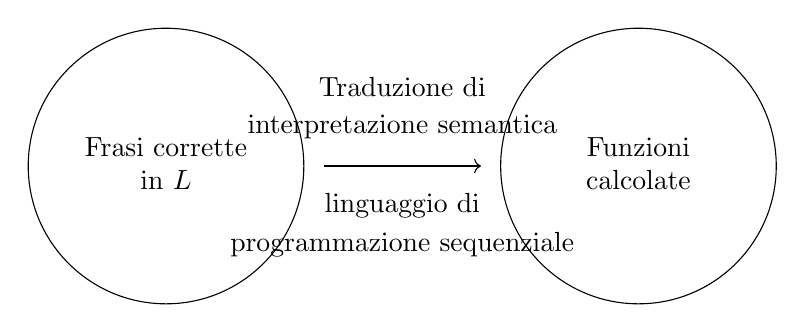
\begin{tikzpicture}
        % Primo cerchio (Frasi corrette in L1)
        \draw (0,0) circle (1.75cm);
        \node at (0,0) {\begin{tabular}{c}
                         Frasi corrette \\ 
                         in \textit{$L$}
                         \end{tabular}};
                         
        % Secondo cerchio (Significato espresso con frasi corrette in L2)
        \draw (6,0) circle (1.75cm);
        \node at (6,0) {\begin{tabular}{c}
                         Funzioni \\ 
                         calcolate \\ 
                         \end{tabular}};
        
        % Freccia tra i due cerchi
        \draw[->] (2,0) -- (4,0);
        \node at (3,1) {Traduzione di};
        \node at (3,0.5) {interpretazione semantica};
        \node at (3,-0.5) {linguaggio di};
        \node at (3,-1) {programmazione sequenziale};
    \end{tikzpicture}
\end{center}

\subsection{Pragmatica}
\dfn{Pregmatica}{
    La \textbf{pragramtica} è un insieme di regole che guidano l'uso e come i contesti influiscono sull'interpretazione di frasi sensate e corrette
}
Ad esempio quando e a chi dare del "tu" o del "lei" quando ci rivolgiamo a delle persone

\subsection{Implementazione}
L'implementazione è \red{l'esecuzione di una frase sintatticamente corretta rispettandone la semantica}

%todo   FINIRE LA FIGURA

\begin{tikzpicture}
    \draw(0,0) circle (1cm);
    
\end{tikzpicture}

La semantica di $P$, è la funzione $f$ che è pure la semantica del programma compilato $Q$, quindi l'implementazione $Q$ di $P$ preseva la semantica di $P$!

\section{Lessico e frasi di un linguaggio}
Innanzi tutto diamo tre definizioni
\dfn{alfabeto}{
    Un \textbf{alfabeto} è un insieme (tipicamente) finito i cui elementi sono detti simboli 
}
Definire l'alfabeto ci porta alla definizione di lessico:
\dfn{Lessico}{
    Il \textbf{lessico} è un insieme di sequenze finite costituite con caratteri o simboli dell'alfabeto
}
Il quale ci porta alla fenizione di frase:
\dfn{frase}{
    Una \textbf{frase} è un insieme sequenze finite contruite con parole del lessico. 
}
È, quindi, facile notare che \red{il lessico è un alfabeto per le frasi}

Si ci si può ora astrarre e definire un linguaggio formale:
\dfn{linguaggio formale}{
    Un \textbf{linguaggio formale} $L$ su alfabeto $A$ è un sottoinsieme di $A^*$ ($L\subseteq A^*$), dove:
    \[
        A^* = \bigcup_{n \geq 0} A^n \quad \text{ dove } A^0 =\{\epsilon\}       
    \]
    e \[
        A^{n+1}= A\cdot A^n \quad n\geq 0    
    \]
    con $A\cdot A^n = \{aw|a\in A \land w \in A^n\}$
}
Si osservi che \red{$A^*$ è un insieme infinito contabile} dato un ordinamento < sui simboli di $A$, possiamo elencare tutt le parole come segue:
\begin{enumerate}
    \item elenco la parola vuota $\epsilon$ ($A^0$)
    \item poi elenco le parole di lunghezza 1 ($A^1$) secondo l'ordinamento <
    
    Es. $a,b,c,\dots$
    \item poi elenco le parole in $A^2$ secondo <
    
    Es. $aa, ab, ac, \dots, ba, bb, bc, \dots$
    \item così via
\end{enumerate}

Anche se l'alfabeto $A$ fosse infinito (quindi $A=\{a_0, a_1, \dots\}$) $A^*$ sarebbe ancora contabile, ovvero esisterebbe la possibilità di elencare tutte le possibili parole in $A^*$. Infatti, \red{esiste una biezione tra $A$ e $\mathbb{N}$} e riguardo ai numeri naturali si sa che:
\begin{itemize}
    \item $\mathbb{N}\times \mathbb{N}$ (prodotto cartesiano) è numerabile. La dimostrazione viene fatta attraverso il \textit{dove-tailing}, una tecnica comune per dimostrare la numerabilità di coppie di numeri naturali. Questa dimostrazione introduce la cosìdetta \textbf{funzione di decodifica}
    
    \[
        f^2(x_1,x_2) =\frac{(x_1+x_2)(x_1+x_2+1)}{2} + x_2
    \]
    che presi due numeri in $\mathbb{N}$ completa la seguente tabella ordinando i numeri naturali in "diagonale"
    
    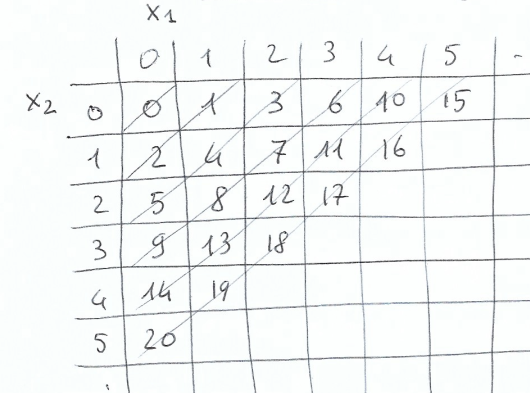
\includegraphics[width=10cm]{funzione_decodifica_tabella.png}

    è pertanto vero, quindi, che
    \[
        f^2:\mathbb{N}\times \mathbb{N}\to \mathbb{N}
    \]
    è biunivoca

    \item $\mathbb{N}^k$ è numerabile. Infatti si può dimostrare attraverso questo algoritmo:
    \[
        f^k(x_1,x_2,\dots,x_k) = \text{ if } (k=2) \text{ then } f^2(x_1,x_2)
        \quad \text{ else } f^2(x_1, f^{k-1}(x_2,\dots,x_k))
    \]
    Ovvero riduce una funzione con $k$ variabili nel dominio ad una serie di funzioni matrioska per ricondurla alla forma $f^2:\mathbb{N}\times\mathbb{N}\rightarrow \mathbb{N}$
    \item $\mathbb{N}^* = \bigcup_{k\geq 0}\mathbb{N}^k$ è numerabile. Infatti:
    \[
        f(x_1,\dots,x_k) = f^2(k,f^k(x_1,\dots, x_k))    
    \]

    
\end{itemize}

\section{Notazioni e definizioni ausiliarie}
Vengono riportate qui alcune definizioni/notazioni
\subsection{Lunghezza}
\dfn{lunghezza}{
    La \textbf{lunghezza} di una parola o stringa è definita per induzione così:
    \begin{itemize}
        \item Caso $|\epsilon|$: $0$
        \item Caso $|aw|$: $1 + |w|$
    \end{itemize}
}
Es: $|abc|=2$ 
\subsection{Concatenazione}
\dfn{Concatenazione}{
    La \textbf{concatenazione} $xy$ tra una stringa $x$ e $y$, è la parola ottenuta giustapponendo $x$ e $y$. Formalmente:
    \[
        w = xy \iff \begin{cases}
            |w|=|x|+|y| \\
            w(j) = x(j) & \text{ per } 1\leq j\leq |x|\\
            w(|x|+j) = x(j) & \text{ per } 1\leq j\leq |y|
        \end{cases}    
    \] 
    Dove $w(j)$ indica il j-esimo simbolo di $w$
}

Questi sono le leggi della concatenazione
\begin{itemize}
    \item Associatività: $x(yz)=(xy)z$
    \item Elemento neutro ($\epsilon$): $x\epsilon = x = \epsilon x$
\end{itemize}

\subsection{Sottostringa}
\dfn{Sottostringa}{
    La stringa $v$ si dive \textbf{sottostringa} di $w \iff \exists x,y \in A^*$ t.c. $w=xvy $ dove $x$ e $y$ possono essere $\epsilon$
}
Si osservi, quindi, che:
\begin{itemize}
    \item Ogni stringa è sottostringa di se stessa
    \item $\epsilon$ è sottostringa di ogni stringa
\end{itemize}

\subsection{Suffisso}
\dfn{suffisso}{
    $v$ si dice \textbf{suffisso} di $w \iff \exists x \in A^x. w=xv$
}
\subsection{Prefisso}
\dfn{prefisso}{
    $v$ si dice \textbf{prefisso} di $w \iff \exists x \in A^x. w=vx$
}
\subsection{Potenza n-esima}
\dfn{potenza n-esima}{
    Si dice \textbf{potenza n-esima} di una stringa $w$ il valore $n\geq 0$ il cui significato è definito per induzione:
    \begin{itemize}
        \item Caso 0: $w^0 = \epsilon$
        \item Caso $n+1$: $w^{n+1}= ww^{n}$
    \end{itemize}
}


\subsection{Linguaggio}
\dfn{linguaggio}{
    Si dice \textbf{linguaggio $L$ su alfabeto $A$} un sottoinsieme $L\subseteq A^*$
}
Vengono riportati qui alcuni esempi
\esempio{
    Se $A=\{a\}$, si possono avere:
    \begin{itemize}
        \item $\emptyset,\{\epsilon\}, \{a,aaa\}$ sono linguaggi finiti
        \item $L_1=\{a^n|\geq 1\}=\{a,aa,aaa,\dots\}=A^*\diagdown \{\epsilon\} $ 
        \item $L_2 =\{a^{2n}|n\geq 0\}=\{\epsilon, aa, aaaa\}$
    \end{itemize}
}
%adssad
\section{Operazione sui linguaggi}
Qui sono elencati le varie operazioni
\subsection{Complemento}
\dfn{complemento}{
    È definito \textbf{complemento} il linguaggio completare ad un linguaggio $L$, ovvero:
    \[
        \overline{L} = \{w\in A^* | w \notin L\} = A^*\diagdown L    
    \]
}
\subsection{Unione e intersezione}
\dfn{unione e intersezione}{
    Ovvi:
    \[
      \begin{array}{l}
            L_1\cup L_2 \{w|w\in L_1 \lor w \in L_2\} \\
            L_1\cap L_2 \{w|w\in L_1 \land w \in L_2\}
      \end{array}
    \]
}

\subsection{Concatenazione}
\dfn{concatenazione}{
    
        È definita \textbf{concatenazione} tale operazione:
        \[
            L_1 \cdot L_2 =\{w_1w_2|w_\in L_1 \land w_2 \in L_2\}
        \]
    
}
Ecco alcuni esempi:
\esempio{
    \begin{itemize}
        \item $L_1 = \{a^n \mid n > 0 \}$ \quad $L_2 = \{b\}$ \\
              $L_1 \cdot L_2 = \{a^n b \mid n > 0\}$
              
        \item $L_1 = \{a^{2n} \mid n > 0 \}$ \quad $L_2 = \{b^m \mid m > 0\}$ \\
              $L_1 \cdot L_2 = \{a^{2n} b^m \mid n, m > 0\}$
              
        \item $L_1 = \{a^m b^n \mid n > 0\}$ \quad $L_2 = \{b^m \mid n > 0\}$ \\
              $L_1 \cdot L_2 = \{a^m b^{n+m} \mid n, m > 0\}$ \\
              \phantom{$L_1 \cdot L_2$} $= \{a^m b^n \mid m \geq n > 0\}$
              
        \item $L_1 = \{a^m \mid m > 1 \}$ \quad $L_2 = \{a^m b^m \mid n > 0 \}$ \\
              $L_1 \cdot L_2 = \{a^{m+n} b^m \mid m > 1, m > 0\}$ \\
              \phantom{$L_1 \cdot L_2$} $= \{a^m b^m \mid m > m > 0\}$
              
        \item $L_1 = \{a b^m \mid n \geq 1\}$ \quad $L_2 = \{a, c\}    \cup \{b^n \mid n \geq 1\}$ \\
              $L_1 \cdot L_2 = \{a b^m a \mid m \geq 1\} \cup \{a b^m c \mid n \geq 1\}$ \\
              \phantom{$L_1 \cdot L_2$} $\cup \{a b^n \mid n \geq 2\}$
              
        \item $A = \{0,1\}$ \\
              $L_1 = \{ w \in A^* \mid w \text{ contiene un numero pari di "0"} \}$ \\
              $L_2 = \{ w \in A^* \mid w = 0y \text{ e } y \in \{1^*\} \}$ \\
              $L_1 \cdot L_2 = \{w \in A^* \mid w \text{ ha un numero dispari di "0"} \}$
    \end{itemize}
}
\subsection{Potenza di un linguaggio}
\dfn{Potenza di un linguaggio}{
    La \textbf{potenza di un linguaggio} viene definita per induzione:
    \begin{itemize}
        \item Caso 0: $L^0 =\{\epsilon\}$
        \item Caso $n+1$: $L\cdot L^n \quad \forall n\geq 0$ 
    \end{itemize}
}

\subsection{Stella di kleene}
\dfn{stella di kleene}{
    Si dice \textbf{stella di kleene}:
    \[
        L^* \bigcup_{n\geq 0} L^n    
    \]
    Oppure 
    \[
        L^+ =   \bigcup_{n\geq 1} L^n   
    \]
    Quest'ultima detta \textbf{chiusura positiva}
}

%asaddsadsa
\section{Definire finitamente un linguaggio}
\subsection{esempio 1: frasi palindrome}
Una frase palindroma è una parola che letta da $sx$ a $dx$ è uguale a se stessa letta da $dx$ a $sx$

Es. "I topi non avevano nipoti"
\begin{itemize}
    \item $A=\{a,b\} \quad L=\{\epsilon, a, b, aa, bb, aba, bab, dots\}$. Come si nota è piuttosto scomodo
    \item Una palindroma può essere: 
        \begin{itemize}
            \item o è la stringa $\epsilon$
            \item oppure a
            \item oppure b
            \item oppure a "palindroma" a
            \item oppure b "palindroma" b
        \end{itemize} 
    \item rappresentazione tramite \textbf{Backus-naur form (BNF)}.
    \[
         \langle P \rangle := \epsilon \mid a\mid b\mid a \langle P \rangle a\mid b \langle P \rangle b   
    \]
    \item  Come \textbf{grammatica}:
    \[
        P\to \epsilon \mid a\mid b\mid aPa\mid bPb    
    \]
    \item definizione ricorsiva in cui:
    \begin{itemize}
        \item $P$ è detto \textit{simbolo non terminale}
        \item $a,b$ sono "simboli terminali"
    \end{itemize}
\end{itemize}
\subsection{Esempio 2}
espressioni aritmetiche formate a partire dalle variabili $a$ e $b$ con gli operatori $\times, +$ e le parantesi $(,)$

Una $expr$ può essere:
\begin{itemize}
    \item \begin{itemize}
        \item la variabile $a$
        \item la variabile $b$
        \item $expr\times expr$
        \item $expr + expr$
        \item ($expr$)
    \end{itemize}
    \item \textbf{bnf}:
      \[
        \langle E \rangle ::= a\mid b\mid \langle E \rangle\times \langle E \rangle \mid \langle E \rangle + \langle E \rangle\mid (\langle E \rangle)
      \]
    \item Grammatica:
    \[
        E\to a\mid b\mid E\times E\mid E+E\mid (E)    
    \]
\end{itemize}

\section{Grammatiche}
Una grammatica è un insieme di regole che descrivono come le parole e le frasi possono essere combinate per formare espressioni valide. Queste regole determinano la struttura sintattica di un linguaggio, specificando come le unità di base (come le parole o i simboli) si connettono per formare frasi o espressioni più complesse. Ogni grammatica \red{segue lo stesso pattern definito} differenziandosi solo per come sono caratterizzate le produzioni.

Quelle più utili sono le cosiddette grammatiche libere (in rapporto tra facilità di analisi ed espressività) 

\dfn{grammatiche libere}{
    Una \textbf{grammatica libera} da contesto è una quadrupla $(NT,T,R,S)$ dove:
    \begin{itemize}
        \item \textbf{NT} è un insieme finito di simboli non terminali
        \item $T$ è un insieme finito di simboli terminali
        \item $S\in NT$ è detto simbolo iniziale
        \item $R$ è un insieme finito di produzione (o regole) della forma:
        \[
            V \to w \text{ dove }V\in NT \land w\in (T\cup NT)^*    
        \]
    \end{itemize}
}

Alcuni esempi:
\esempio{
    \[
        G= (\{S\}, \{a,b,+,\times\}, S, R)
    \]
    Con 
    \[
        R=\{S \to a, S \to b, S\to S+S, S\to S\times S\}    
    \]
}

\section{Derivazioni}
\dfn{derivazione immediata}{
    Data $G=(NT, T,R,S)$ libera dal contesto, diciamo che da $v$ si \textbf{deriva immediatamente}  $w$, e lo denotiamo con $v \Rightarrow w$, se:
    \[
        \frac{v =xAy \quad (A\to z )\in R \quad w=xzy}{v\Rightarrow w}    
    \]
    
}
\dfn{derivazione}{
    Diciamo che da $v$ si \textbf{deriva} $w$ (o anche "$v$ si riscrive in $w$"), e lo deontiamo con $v \Rightarrow^* w$, se esiste una sequenza finita (evenutalmente vuota) di derivazione immediate 
    \[
        v \Rightarrow w_0 \Rightarrow w_1 \Rightarrow \dots \Rightarrow w
    \]
    Cioè:
    \[
        \frac{ }{v \Rightarrow^* v} \quad \frac{v\Rightarrow^* w \quad w\Rightarrow z}{v\Rightarrow^* z}    
    \]
    Dove $\Rightarrow^*$ è la chiusa riflessiva e transitiva della relazione $\Rightarrow$
}

\section{Linguaggio Generato}
\dfn{Linguaggio Generato}{
    Il \textbf{linguaggio generato} da una grammatica $<G=(NT, T ,R,S)$ è l'insieme
    \[
        L(G) = \{w\in T^*|S \der w\}
    \]
}

\subsection{Algoritmo di Naif}

Data una grammatica $G$ è opportuno chiedersi come si fa a determinare un linguaggio $L(G)$ e a verificare se $w\in L(G)$. La domanda può essere complessa, tuttavia in casi semplici ci viene in aiuto \textbf{l'algoritmo di Naif} che consiste nel partire da $S$ e provare ad applicare in tutti i modi possibili le produzione (regole) per trovare una derivazione che generi $w$

In certi casi questa verifica è semplice

\esempio{
    \begin{itemize}
        \item 
            Sia $G_3$ con $S\to aSb|ab$

            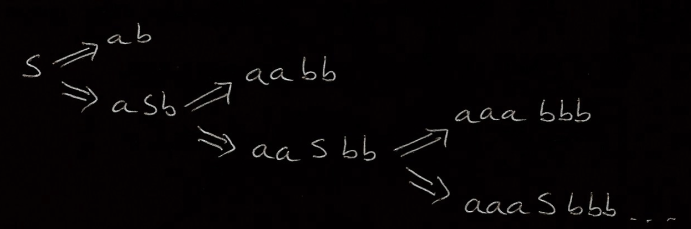
\includegraphics[width=10cm]{alberello.png}
        
            In questo esempio è facile determinare che $L(G_3)=\{a^n b^n|n\geq 1\}$
        \item 
            Sia $G_1 \to aAb \text{ e }A\to aAb\mid \epsilon$ 

            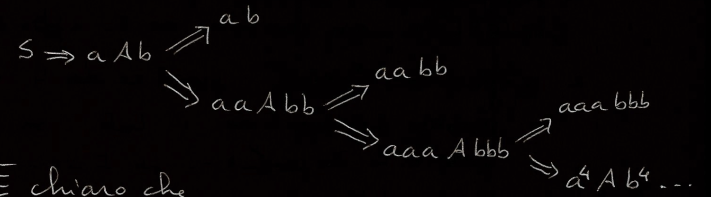
\includegraphics[width=10cm]{alberello_1.png}

            Quindi $L(G_1) = \{a^nb^n\mid n\geq 1\}$
    \end{itemize}

    Si può notare che $G_1 \text{ e } G_3$ sono grammatiche equivalenti perché $L(G_1)=L(G_3)$

    In generale \red{esistono grammatiche diverse che generano lo stesso linguaggio}
    
}

\section{Alberi di derivazione}

Per rappresentare graficamente e semplicemente una certa grammatica esiste uno strumento utilissimo, ovvero l'albero di derivazione

\dfn{albero di derivazione}{
    Data una grammatica libera $G= ( NT, T, S, R)$, un albero di derivazione (o di parsing) è un albero ordinato in cui: 
    \begin{itemize}
        \item Ogni nodo è etichettato con un simbolo in $NT \cup \{\epsilon \} \cup T$
        \item la radice è etichettata con $S$
        \item ogni nodo interno è etichettato con un simbolo in $NT$ 
        \item se il nodo $n$
        \begin{itemize}
            \item ha etichetta $A\in NT$ 
            \item i suoi figli sono nell'ordine $m_1,\dots, m_k$ con ,etichetta $x_1,\dots, x_k$ (in $NT\cup T$), allora
            \[
                A \to x_1, \dots , x_k \text{ è una produzione in R }
            \]
        \end{itemize}
        \item se il nodo $n$ ha etichetta $\epsilon$, allora $n$ è una foglia, è figlio unico e, dato $A$ suo padre, $A\to \epsilon$ è una produzione di $R$
        \item se inoltre ogni nodo foglia è etichettato su $T\cup\{\epsilon\}$ è una produzione di $R$
        \item se inoltre ogni nodo foglia è etichettato su $T\cup\{\epsilon\}$, allora l'alberello di derivazione corrisponde ad una derivazione completa
    \end{itemize}
}

Un albero di derivazione, quindi, \red{riassume tante derivazioni diverse ma tutte equivalenti} (ovvero generano lo stesso albero)
\esempio{
    Consideriamo la grammatica 
    \[
        s\to a|b|c|S+S|S \times S
    \]
    Inoltre si consideri la derivazione
    \[
        S \Rightarrow \underbar{S}+S \Rightarrow \underbar{S}\times S + S \Rightarrow a \times \underbar{S}+S \Rightarrow a \times b + \underbar{S} \Rightarrow a\times b + c
    \]
    Allora il suo albero di derivazione è:
    \begin{center}
        
        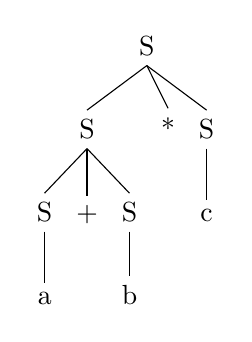
\begin{tikzpicture}
            \Tree [.S 
                    [.S [.S a ] + [.S b ] ] 
                    * 
                    [.S c ]
                ]
        \end{tikzpicture}
    \end{center}
}
Si osservi inoltre che l'albero di derivazione fornisce informazioni semantiche: "quali operandi per quali operatori" e possono essere riassunti nei cosiddetti \red{alberi sintattici}, tipo
\begin{center}
    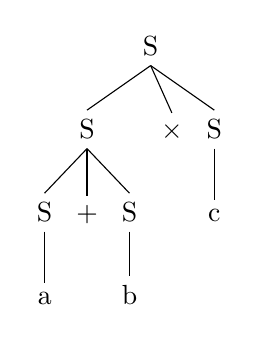
\begin{tikzpicture}
        \Tree [.S 
                [.S [.S a ] + [.S b ] ] 
                $\times$
                [.S c ]
             ]
    \end{tikzpicture}
    e
    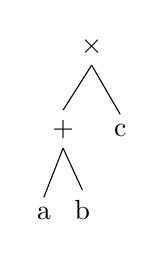
\begin{tikzpicture}
            \Tree [.$\times$ 
                    [
                        .+ 
                        [.a ] 
                        [.b ] 
                    ] 
                    [
                        .c 
                    ] 
                  ]
    \end{tikzpicture}    
\end{center}

        


\teorema{
    Una stringa $w\in T^*$ appartiene a $L(G)$ sse ammette un albero di derivazione completo (le cui foglie, lette da sx a dx diano la stringa $w$) cioè visita in ordine anticipato tralasciando i nonterminali
}


\subsection{Ambiguità}
Per spiegare cos'è l'ambiguità partiamo con un esempio
\esempio{
    Si consideri la seguente grammatica
    \[
        S\to a|b|c|S+S|S\times S    
    \]
    Si hanno due diverse derivazioni per $a\times b + c$:
    \begin{enumerate}
        \item  $S \Rightarrow \underbar{S}+S \Rightarrow \underbar{S}\times S + S \Rightarrow a \times \underbar{S}+S \Rightarrow a \times b + \underbar{S} \Rightarrow a\times b + c$
        
        con l'albero: 
        \begin{center}
            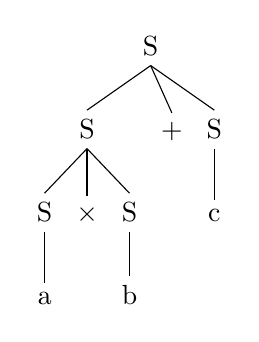
\begin{tikzpicture}
                \Tree [.S 
                        [.S [.S a ] $\times$ [.S b ] ] 
                        + 
                        [.S c ]
                    ]
            \end{tikzpicture} 
        \end{center}
        \item $S \Rightarrow \underbar{S}\times S \Rightarrow a \times \underbar{S} \Rightarrow a  \times \underbar{S} + s \Rightarrow a\times b + \underbar{S} \Rightarrow a\times b + c$
        
        Con l'albero:

        \begin{center}
            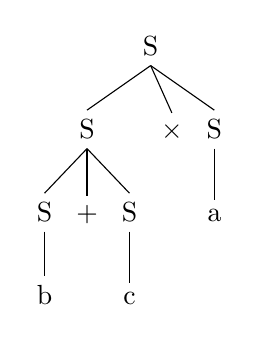
\begin{tikzpicture}
            \Tree [.S 
                [.S 
                    [.S b ] 
                    + 
                    [.S c ] 
                ]
                $\times$
                [.S a ] 
            ]
            \end{tikzpicture}
        \end{center}
    \end{enumerate}

}

Per questa grammatica, la stringa $a\times b + c $ ha più di un albero di derivazione in questi casi si dice che la grammatica è quindi \textbf{ambigua} e \red{inutilizzabile per dare semantica a   $a\times b + c $}. Bisogna utilizzare grammatiche non ambigue, o manipolare grammatiche ambigue per disambiguarle

\subsubsection{Grammatica ambigua}
\dfn{Grammatica ambigua}{
    Una grammatica libera $G$ è \textbf{ambigua} se $\exists w \in L(G)$ che ammette più alberi di derivazione
}
\dfn{Linguaggio ambiguo}{
    Un linguaggio $L$ è \textbf{ambiguo} se tutte le grammatiche $G$, tali che $L(G)=L$, sono ambigue
}

Alcune grammatiche possono essere manipolate di modo da \begin{itemize}
    \item rimuovere l'ambiguità
    \item generare lo stesso linguaggio
\end{itemize}
In altre, invece, ti tieni l'ambiguità (non è possibile rimuoverla (cazzo)) 

\subsection{Rimuovere l'ambiguità}
Questa CAZZATA viene spiegata con solo degli esempi

\esempio{
    Sia $S$ la grammatica
    \[
        S\to a\mid b\mid c\mid S+S\mid S\times S \text{ è ambigua!}       
    \]
    Problemi: \begin{itemize}
        \item Precedenza del * rispetto al + in modo che $a\times b + c$ sia interpretato come:
        \begin{center}
            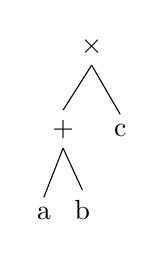
\begin{tikzpicture}
                \Tree [.$\times$ 
                        [
                            .+ 
                            [.a ] 
                            [.b ] 
                        ] 
                        [
                            .c 
                        ] 
                      ]
            \end{tikzpicture}  
        \end{center}
        \item associatività del $+$ e del $\times$
        \begin{center}
            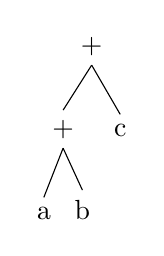
\begin{tikzpicture}
            \Tree [.+
                    [
                        .+ 
                        [.a ] 
                        [.b ] 
                    ] 
                    [
                        .c 
                    ] 
                  ]
        \end{tikzpicture}  
        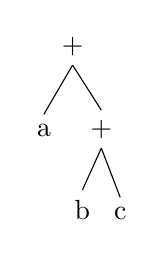
\begin{tikzpicture}
            \Tree [.+
                    [
                        .a
                    ] 
                    [
                        .+ 
                        [.b ] 
                        [.c ] 
                    ] 
                  ]
        \end{tikzpicture}  
    \end{center}
        
        $a+b+c$ ovvero bisogna scegliere l'associatività a dx o sx
        
    \end{itemize}

    Un modo per eliminare questa ambiguità è definire la grammatica così:
    \[
        e\to E+T\mid T \quad T\to A \times T\mid A \quad A \to a\mid b\mid c\mid(E)    
    \]
}

\chapter{Struttura di un compilatore, semantica statica, semantica dinamica}
\section{Vincoli contestuali}
\dfn{vincoli sintattici contestuali}{
    I \text{vincoli sintattici contestuali} sono termini o parole riservate non esprimibili per mezzo di grammatiche libere (perché non possono descrivere vincoli vincoli che dipendono dal contesto) che bisogna evitare di considerare quando si esegue il codice
}

Tradizionalmente i vincoli sintattici contestuali appartengono alla sintassi, ma nel gergo dei $LP$, si intende:
\begin{itemize}
    \item \textbf{Sintassi}: quello che si \red{scrive per mezzo di Grammatiche Libere}
    \item \textbf{semantica} tutto il resto $\dots$
\end{itemize}  

Pertanto \red{i vincoli contestuali sono dunque vincoli semantici, detti di } \textbf{semantica statica} cioè vincoli che possono essere verificati ispezionando il codice \red{senza mandare il programma in esecuzioni}

Il compilatore delega questi controlli di semantica statica alla cosiddetta \textbf{analisi semantica}
\section{Semantica statica}
\dfn{Semantica statica}{
    Per \textbf{semantica statica} si intende l'insieme di quei controlli che possono essere fatti sul testo del programma senza eseguirlo
}
\esempio{
    \texttt{int A;}\\
    \texttt{bool B}\\
    \texttt{A := B} (errore di tipo)
}
\section{semantica dinamica}
Per \textbf{semantica dinamica} si intende una rappresentazione formale dell'esecuzione del programma, la quale può mostrare errori durante l'esecuzione
\esempio{
    \texttt{read(A);}\\
    \texttt{B := $\frac{10}{A}$} (Se $A=0$ si da un errore in esecuzione. F)
}

Staticamente non si può sapere l'errore perché la sua occorrenza \red{dipende dall'input dell'utente che fornirà durante l'esecuzione del programma}

Per implementare una semantica dinamica occorre fornire un modello matematico che descriva indipendentemente dall'architettura su cui il programma viene eseguito, il "comportamento del programma"

\esempio{
    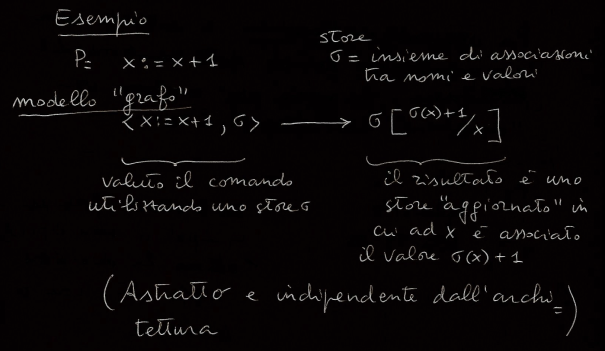
\includegraphics[width=10cm]{esempio_semantica_dinamica.png}
}

\subsection{Utilità della semantica dinamica}
A chi serve la semantica dinamica?

\begin{itemize}
    \item \textbf{Al programmatore}: \textit{ANALISI DEL PROGRAMMA}
    \begin{itemize}
        \item deve sapere esattamente cosa debba fare il suo programma
        \item deve poter dimostrare proprietà del suo programma (ad es.: "termina sempre per ogni possibile input?")
    \end{itemize}
    
    \item \textbf{Al progettista del linguaggio}:
    \begin{itemize}
        \item strumento di specifica del linguaggio
        \item deve poter dimostrare proprietà del linguaggio (ad es.: "è Turing-completo?")
    \end{itemize}
    
    \item \textbf{All'implementatore del linguaggio}:
    \begin{itemize}
        \item riferimento per dimostrare la correttezza dell'implementazione
        
        Infatti \red{un compilatore è corretto quando preserva la semantica dinamica}, quindi per dimostrare che un compilatore è corretto serve avere una semantica per il linguaggio sorgente e per il linguaggio oggetto
    \end{itemize}
\end{itemize}

\subsection{definire la semantica}
Per definire la semantica si utilizzano due tecniche principali: 
\begin{itemize}
    \item \textbf{operazionale}: (macchina astratta a stati e transizioni)
   
    Ovvero si costruisce una specie di automa che, passo a passo, mostra l'effetto dell'esecuzione delle varie istruzioni. \red{vi è una maggiore enfasi su COME si calcola}

    \item \textbf{Denotazionale}: si associa ad ogni programma sequenziale una funzione da input ad output (incluse strutture ausiliarie e memoria). \red{vi è una maggiore enfasi su COSA si calcola}
        
\end{itemize}
\section{Pragmatica nella descrizione di un linguaggio}
\dfn{Pragmatica nella descrizione di un linguaggio}{
    si definisce \textbf{pragmatica nella descrizione di un linguaggio} insieme di regole sul modo in cui è meglio usare le istruzioni a disposizione
}
Esempietti:
\esempio{
    \begin{itemize}
        \item evitare le istruzioni di salto quando possibile
        \item usare le variabili di controllo del \texttt{for}  solo a quello scopo
        \item scelta della modalità più appropriata di passaggio di paramatri ad una funzione
        \item scelta tra iterazione determinata (\texttt{for}) e indeterminata (\texttt{while})
    \end{itemize}
}
\section{
    implementazione
}
\dfn{implementazione}{
    Per \textbf{implementazione} si intende la scrittura di un compilatore per una macchina ospite già realizzata, costruendo così una macchina astratta per il linguaggio
}

\subsection{Correttezza dell'implementazione}

Per far sì che un compilatore sia corretto occorre \red{dimostrare che il programma preservi la semantica}, ovvero il programma sorgente e quello oggetto calcolino la stessa funzione 

\subsection{Struttura di un compilatore}
\begin{tikzpicture}[node distance=1.8cm]

    % Blocchi principali
    \node (start) [process] {Programma sorgente};
    \node (lex) [process, below of=start] {Analisi Lessicale};
    \node (tokens) [process, below of=lex] {Lista di Token};
    \node (syn) [process, below of=tokens] {Analisi Sintattica};
    \node (tree) [process, below of=syn] {Albero di derivazione};
    \node (sem) [process, below of=tree] {Analisi Semantica};
    \node (augTree) [process, below of=sem] {Albero derivazione aumentato};
    \node (interForm) [process, below of=augTree] {Generazione forma intermedia};
    \node (form) [process, below of=interForm] {Forma intermedia};
    \node (opt) [process, below of=form] {Ottimizzazione};
    \node (optForm) [process, below of=opt] {Forma intermedia ottimizzata};
    \node (codeGen) [process, below of=optForm] {Generazione del codice};
    \node (objectCode) [process, below of=codeGen] {Codice oggetto};
    
    % Frecce principali
    \draw [arrow] (start) -- (lex);
    \draw [arrow] (lex) -- (tokens);
    \draw [arrow] (tokens) -- (syn);
    \draw [arrow] (syn) -- (tree);
    \draw [arrow] (tree) -- (sem);
    \draw [arrow] (sem) -- (augTree);
    \draw [arrow] (augTree) -- (interForm);
    \draw [arrow] (interForm) -- (form);
    \draw [arrow] (form) -- (opt);
    \draw [arrow] (opt) -- (optForm);
    \draw [arrow] (optForm) -- (codeGen);
    \draw [arrow] (codeGen) -- (objectCode);
    
    % Tabelle di simboli e gestore degli errori
    \node (symTab) [process, left of=tree, xshift=-3cm, yshift=-1cm] {Tabella dei Simboli};
    \node (errManager) [process, right of=tree, xshift=3cm, yshift=-1cm] {Gestore degli errori};
    
    % Frecce verso la tabella dei simboli
    \draw [arrow] (lex.west) -- ++(-1,0) |- (symTab.north);
    \draw [arrow] (sem.west) -- ++(-1,0) |- (symTab.south);
    
    % Frecce verso il gestore degli errori
    \draw [arrow] (tree.east) -- ++(1,0) |- (errManager.north);
    \draw [arrow] (augTree.east) -- ++(1,0) |- (errManager.south);
    
\end{tikzpicture}

\section{fasi principali della compilazione}
\subsection{analisi lessicale (scanner)}
L'analisi lessicale spezza il programma sorgente nei componenti sintattici primitivi chiamati "tokens" (identificatori, numeri, operatori, parametri, parole riservate)
\begin{itemize}
    \item controlla solo che il lessico sia ammissibile 
    \item riempie parzialmente la tabello dei simboli per gli identificatori di variabili, procedure funzioni $\dots$
\end{itemize}

Per realizzare uno scanner avremo bisogno di studiare:
\begin{itemize}
    \item \textbf{grammatiche regolari}
    \item \textbf{espressioni regolari}: un formalismo usato per descrivere i linguaggi generati da grammatiche regolari 
    \item \textbf{automi a stati finiti}: uno strumento che permette di riconoscere i linguaggi regolari
\end{itemize}

\subsection{analisi sintattica (parser)}
A partire dalla lista di tokens, generata dallo scanne, il parser produce l'albero di derivazione del programma, riconoscendo se le frasi sono sintatticamente corrette

Ad esempio controlla che: 
\begin{itemize}
    \item le parentesi siano bilanciate: \texttt{((a)+b)))}
    \item che i comandi siano composti secondo le regole grammaticali \texttt{if(x=5) then then x:=3}
\end{itemize}

Per realizzare un Parser, avremo bisogno di:
\begin{itemize}
    \item grammatiche libere dal contesto
    \item automi a pila
\end{itemize}

\subsection{Analisi semantica}
l'analisi semantica \red{esegue dei controlli di semantica statica} (ovvero sintattici contestuali) per rilevare eventuali errori semantici

Arricchisce l'albero di derivazione generato dal Parser con informazioni sui tipi, verifica i tipi negli assegnamenti, parametri attuali vs. formali, dichiarazione e uso di variabili e genera eventuali errori

\subsection{Generazione della forma intermedia}
Genera codice scritto in un \textbf{linguaggio intermedio} indipendente dall'architettura, facilmente traducibile nel linguaggio macchina di varie macchine diverse. Nel generare questo codice intermedio si esegue la struttura dell'albero sintattico, ricavato dall'albero di derivazione

\subsection{Ottimizzazione}
Si effettuano ottimizzazioni nel codice intermedio per renderlo più efficiente
\begin{itemize}
    \item rimozione di codice inutile (dead code) 
    \item espansione in linea di chiamate di funzioni
    \item fattorizzazione di sottoespressioni
    \item mettere fuori dai cicli sottoespressioni che non variano
\end{itemize}

Alla fine si ottiene un codice intermedio \textbf{ottimizzato}
\subsection{Generazione del codice}
Viene generato codice per una specifica architettura (include anche l'assegnazione dei registri e ottimizzazioni specifiche macchine)

\subsection{Tabella dei simboli}
Memorizza le informazioni sui nomi presenti nel programma (identificatori di variabili, funzioni, procedure)

Es: per le matrice mette, come attributo la dimensione e il tipo dei suoi elementi 

\section{semantica operazionale strutturata}
\subsection{Definizione di un linguaggio a cui dare semantica}
lA \textbf{semantica operazionale strutturata} È utilizzata per descrivere come ogni singola istruzione o espressione in un linguaggio modifica lo stato di un sistema in termini di transizioni di stato

Il suo \textbf{linguaggio} viene \red{definito tramite sintassi atratta semplice ed intuitiva, ma ambigua} ed una stringa viene sempre accoppiata ad un albero sintattico (non ambiguo)

Alcuni elementi fondamentali del linguaggio vengono definiti attraverso \textbf{insiemi di base}:
\begin{itemize}

    \item \textbf{Booleani}: l'insieme dei valori booleani è composto da due valori: \texttt{$\{$tt,ff$\}$}. Le metavariabili sono $t,t_1,t'\in\mathbb{T}$

    \item \textbf{numeri naturali}: $\{0,1,2,\dots\} \quad n,m,p\in\mathbb{N}$
    
    \item \textbf{variabili}: ${a,b,c,\dots, z} \quad v\in Var$
\end{itemize}

Per descrivere espressioni più complesse, vengono definiti alcuni \textbf{insiemi derivati} utilizzando la notazione BNF (Backus-Naur Form)
\begin{itemize}
    \item \textbf{espressioni aritmetiche} (\texttt{exp}):
        \[
            e::= m | v | e+e|e-e|e*e    
        \]
    \item \textbf{espressioni booleane} (\texttt{Bexp}):
    \[
        b::= t|e=e|b \text{ or } b | \lnot b    
    \]
    \item \textbf{Comandi} \texttt{Com}:
    \[
        c::=\text{skip}|v:=e |c;c|\text{ while }b\text{ do }c|\text{if }b\text{ then }c\text{ else }c    
    \]
\end{itemize}

Questo tipo di sintassi è piuttosto semplice ma è ambigua, \red{per una sintassi non ambigua ne dovrei costruire una completa, ma molto più complicata} (dovrei gestire le precedenze, le parentesi ecc...) ma non serve nel dare una semantica in un linguaggio di programmazione perché un \red{parser (analizzatore sintattico) prende in input un programma scritto in sintassi concreta (non ambigua) e restituisce un albero sintattico di sintassi astratta} (quella che stiamo appena definendo), pertanto, nel dare semantica possiamo partite dagli alberi di sintassi astratta (ambigua) e ignorare la parte di anali del parser

\esempio{
    Riportiamo qui un esempio di sintassi astratta.

    Che tipo di albero sintattico vogliamo intendere con la seguente espressione? 
    \[\text{ while }b\text{ do }c_1;c_2\]
    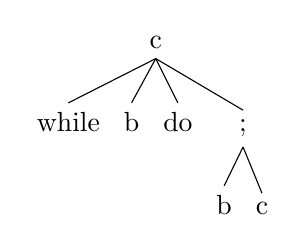
\begin{tikzpicture}
        \Tree [.c
                    [
                        .while
                    ]
                    [
                        .b
                    ] 
                    [
                        .do
                    ]
                    [
                        .; 
                        [.b ] 
                        [.c ] 
                    ] 
                ]
    \end{tikzpicture}
    %TODO LEZ10 P. 2 COMPLETARE
}

\section{Dare semantica ad un linguaggio}
Entriamo nel vivo del discorso, ma prima definiamo, per ogni categoria sintattica (cioè \texttt{Exp}, \texttt{Bexp}, \texttt{Com})un modello detto \textbf{sistema di transizione} che è fondamentalmente un "grafo" di stati

\dfn{sistema di transizione}{
    Un \textbf{sistema di transizione} è una tripla $\langle \Gamma, T, \rightarrow \rangle$ dove
    \begin{itemize}
        \item $\Gamma$ è l'insieme di stati (o configurazione)
        \item $T \subseteq \Gamma$ è l'insieme degli stati terminali (ovvero tutti quegli stati in cui il calcolo è stato terminato con successo)
        \item $\rightarrow \subseteq \Gamma\times\Gamma$ è la relazione di transazione che prende in input uno stato $\in \Gamma$ e restituisce un'altro stato $\in\Gamma$
    \end{itemize}
}
Una computazione a partire dallo stato $\gamma_0$ è una sequenza $\gamma_0\rightarrow\gamma_1\rightarrow\gamma_2\rightarrow\dots$ che può essere finita o infinita, invece con $\rightarrow^*$ si indica la chiusura riflessiva  e transitiva di $\rightarrow$, ovvero:
\[
    \frac{}{\gamma \rightarrow^* \gamma} \quad \frac{\gamma \rightarrow^* \gamma' \quad \gamma' \rightarrow \gamma''}{\gamma \rightarrow^* \gamma''}    
\]
ovvero si può raggiungere da uno stato \red{$\gamma$ uno stato $\gamma''$ in più passi}

\esempio{
    \begin{center}
        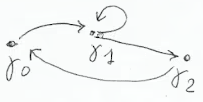
\includegraphics[width=10cm]{rappr_grafica_grafo.png}
    \end{center}
    Questa è una rappresentazione grafica di un grafo in cui i nodi sono gli stati e gli archi le transizioni
}

Se voglio definire la semantica (se voglio usare questo tipo di struttura) del linguaggio con la sintassi definita prima occorre definire uno stato di transazione specifico per \texttt{Exp}, per \texttt{Bexp} e per \texttt{Com}

Vi sono tuttavia \red{diversi problemucci}, del tipo:
\begin{enumerate}
    \item $\Gamma$ è di solito un insieme infinito contabile, allora vi è la \red{necessità di trovare una rappresentazione finita ed implicita attraverso grammatiche}. Questo vuol dire che $\Gamma$ coincide con uno dei linguaggi delle 3 categorie sintattiche (ovvero \texttt{Exp}, \texttt{Bexp}, \texttt{Com})
    \esempio{
        \[
            \Gamma_e = \{\langle e,\sigma \rangle | e \in Exp, \sigma \in Store\}
        \]
        Dove $\sigma$ è una funzione che associa ad ogni variabile un numero naturale, perché lo stato del mio sistema è una coppia in cui la prima parte indica l'espressione che devo valutare, la seconda componente è lo store che indica il valore dell'espressione   
    }
    \item $\rightarrow \subseteq \Gamma\times\Gamma$ è una relazione costituita da infinite coppie $\gamma \rightarrow \gamma'$, anche qui vi è la necessità di trovare una rappresentazione finita ed implicita come minima relazione che soddisfa \red{un certo insieme finito di assiomi e regole di inferenza}, quindi la semantica non è che un insieme di regole di inferenza che mi indicano in modo calcolare le transizioni che mi portano ad eseguire un certo comando
    \item per dare significato alle variabili (che posono solo assumere valore su $\mathbb{N}$) è necessario introdurre uno \textbf{store} $\sigma:Var\rightarrow \mathbb{N}$, come funzione che associa ad ogni variabile un valore
    \[
        \sigma = \{x_1/n_1, x_2/n_2, \dots, x_k/n_k\}    
    \]
    Se supponiamo che $var = \{x_1, x_2, \dots, x_k\}$
\end{enumerate}

\subsection{Semantica delle espressioni artimetiche}
Adesso introduciamo la \textbf{Semantica delle espressioni aritmetiche}, un tipo di semantica operazionale. Deve ovviamente avere un sistema di transizione $\langle \Gamma_e, T_e, \rightarrow_e \rangle$ dove:
\begin{itemize}
    \item $\Gamma_e = \{ \langle e, \sigma \rangle | e \in Exp, \sigma\in Store\}$
    \item $T_e = \{ \langle n, \sigma \rangle | n \in \mathbb{N}, \sigma\in Store\}$
    \item La relazione $\rightarrow_e$ è definita come la minima relazione che soddisfa gli assiomi e le regole di inferenza qui sotto:
    \begin{enumerate}
        \item \textbf{Variabile}:
        \[
        \frac{}{\langle v, \sigma \rangle \rightarrow_e \langle \sigma(v), \sigma \rangle}    
        \]
        Ovvero il tuo stato terminale sarà il numero della variabile $v$ indicato dallo Store (inoltre $\sigma$ rimane inalterato). Quindi valuto ciò che $v$ vale in $\sigma$
        \item \textbf{Somma 1}:
        \[
            \frac{\langle e_0, \sigma \rangle \rightarrow_e \langle e_0', \sigma' \rangle}{\langle e_0 + e_1, \sigma \rangle \rightarrow_e \langle e_0' + e_1, \sigma' \rangle}
        \]

        Nel momento in cui riesco a fare un passo di valutazione da $e_0$ a $e_0'$ alterando anche lo stato dello store da $\sigma$ a $\sigma'$ questa trasformazione si anche applicare durante una somma, in altre parole l’espressione si semplifica o riduce (ad esempio, una variabile viene sostituita con il suo valore), e nel contempo lo stato della memoria potrebbe essere aggiornato se l’espressione stessa comporta una modifica ai valori delle variabili

        \item \textbf{Somma 2}:
        \[
            \frac{\langle e_1, \sigma \rangle \rightarrow_e \langle e_1', \sigma' \rangle}{\langle m + e_1, \sigma \rangle \rightarrow_e \langle m + e_1', \sigma' \rangle}
        \]
        Stessa roba ma con un numero $m$
        \item \textbf{Somma 3}:
        \[
            \frac{}{\langle m+m', \sigma \rangle \rightarrow_e \langle P, \sigma \rangle}   \quad \text{ dove } P = m+m' 
        \]
        \item \textbf{Sottrazione 1}:
        \[
            \frac{\langle e_0, \sigma \rangle \rightarrow_e \langle e_0', \sigma' \rangle}{\langle e_0 - e_1, \sigma \rangle \rightarrow_e \langle e_0' - e_1, \sigma' \rangle}
        \]
        \item \textbf{Sottrazione 2}:
        \[
            \frac{\langle e_1, \sigma \rangle \rightarrow_e \langle e_1', \sigma' \rangle}{\langle m - e_1, \sigma \rangle \rightarrow_e \langle m - e_1', \sigma' \rangle}
        \]
        \item \textbf{Sottrazione 3}:
        \[
            \frac{}{\langle m - m', \sigma \rangle \rightarrow_e \langle p, \sigma \rangle}
        \]
        
   

    \end{enumerate}

    Si noti come la somma e la sottrazione prima valutano la sottoespressione di sinistra ($e_0$) con somma/sottrazione 1 poi, se questa s'è mutata in numero, valutano la sottoespressione di destra ($e_1$) con somma/sottrazione 2 ed infine, se questa s'è mutata in un numero, viene fatta la somma/sottrazione finale con somma/sottrazione 3

    \esempio{
        Esempietto per valutare $\langle (x+2)-y, \{x/5, y/3\} \rangle$:
        
        \begin{center}
            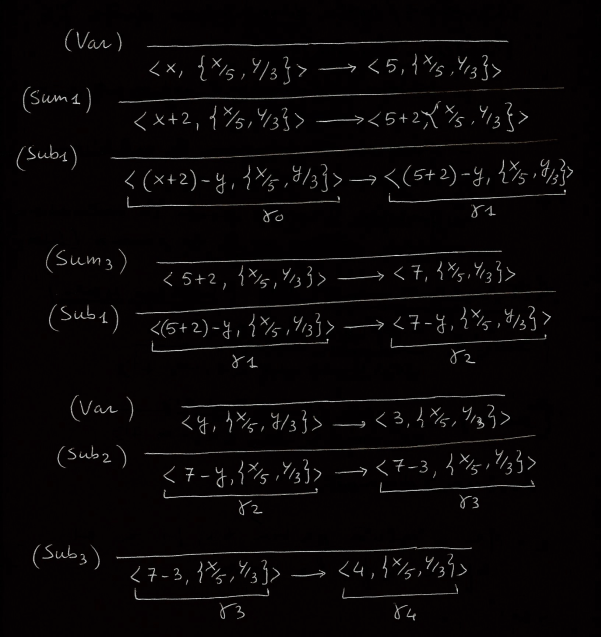
\includegraphics[width=10cm]{esempio_di_transizione.png}
        \end{center}

        Si ha, quindi, che $\gamma_0\rightarrow\gamma_1\rightarrow\gamma_2\rightarrow\gamma_3\rightarrow\gamma_4\in T_e$ cioè $\langle (x+2)-y, \{x/5, y/3\} \rangle \rightarrow^*\langle 4, \{x/5, y/3\} \rangle$
    }
\end{itemize}

\teorema{
    Vogliamo dimostrare che $\rightarrow_e$ è deterministico, ovvero:
    \[
        \gamma\rightarrow_e\gamma'\text{ e } \gamma\rightarrow_e\gamma''\text{, allora }\gamma'=\gamma''\quad \forall \gamma,\gamma',\gamma''  
    \]

    In altre parole significa che \red{da ogni transizione esce al più una transizione}, mai più di una
}
\pf{dimostrazione}{
    mi riduco a dimostrare che $(\inside{e,\sigma}\rightarrow_e \gamma' \land \inside{e,\sigma}\rightarrow_e\gamma'')\Rightarrow\gamma'=\gamma''$ 

    Procedo per induzione strutturale, con HP $(\inside{e,\sigma}\rightarrow_e \gamma' \land \inside{e,\sigma}\rightarrow_e\gamma'')\Rightarrow\gamma'=\gamma''$.
    \begin{enumerate}
        \item $e=m\in \mathbb{N}$: se $\inside{e,\sigma}\nrightarrow_e e$ allora la conclusione è vera perché la premessa è falsa
        \item $e=v\in Var$: Per la regola (Var), l'unica transizione derivabile per $\inside{v,\sigma}$ è $\inside{v,\sigma}\rightarrow_e \inside{\sigma(v), \sigma}$ poiché $\sigma$ è una funzione (cioè $\sigma(v)$ è univoco) e la sola regola (Var) è applicabile allora per forza $\inside{\sigma(v), \sigma} = \sigma'$ e $\inside{\sigma(v), \sigma}=\sigma''$ quindi $\gamma'=\gamma''$
        \item $e = e_0 + e_1$:
            Supponiamo che $\inside{e_0+e_1,\sigma}\rightarrow\gamma'$ e $\inside{e_0+e_1,\sigma}\rightarrow\gamma''$
            
            Ci sono 3 sottocasi da esaminare in accordo nel modo in cui derivo  $\inside{e_0+e_1,\sigma}\rightarrow\gamma'$:
            \begin{enumerate}
                \item  $\inside{e_0,\sigma}\rightarrow\inside{e_0',\sigma'}$ e $\gamma'=\inside{e_0' + e_1, \sigma'}$
                in questo caso ho che $e_0 \notin \mathbb{N}$ e la regola che ho applicato è \texttt{Somma 1}. 
                Allora se $\inside{e_0+e_1, \sigma}\rightarrow \gamma''$ è necessario che $\inside{e_0, \sigma}\rightarrow \inside{e_0'', \sigma''}$ e che $\gamma''=\inside{e_0''+e_1, \sigma''}$.

                Tuttavia per (HP) si ha che $\inside{e_0',\sigma'} = \inside{e_0'',\sigma''}$ pertanto deve essere che $e_0' = e_0''$ e $\sigma' = \sigma''$, da cui discende $\gamma' = \gamma''$
                \item $e_0 = m \in \mathbb{N}$ ed $\inside{e_1, \sigma}\rightarrow\inside{e_1', \sigma'}$ 
                Caso analogo al precedente, dato che ho che $e_1\notin\mathbb{N}$ e la regola che ho applicato è \texttt{Somma 2}. Allora se $\inside{e_0 + e_1, \sigma}\rightarrow \gamma''$, è necessario che $\inside{e_1, \sigma}\rightarrow \inside{e_1'',\sigma''}$ e $\gamma'' = \inside{e_0+e_1'',\sigma''}$. Tuttavia per (HP) si ha che $\inside{e_1',\sigma'} = \inside{e_1'',\sigma''}$ pertanto deve essere che $e_1' = e_1''$ e $\sigma' = \sigma''$, da cui discende $\gamma' = \gamma''$
                \item $e_0 \in \mathbb{N}$ ed $e_1\in \mathbb{N}$
                In questo caso, solo \texttt{Somma 3} è applicabile, ottenendo una sola passibile transizione:
                \[
                    \inside{e_0+e_1,\sigma} \to\inside{P, \sigma} \text{ dove } P = e_0+e_1
                \] 
                Quindi la tesi segue:
                \[
                    \inside{e_0+e_1,\sigma}\to\gamma'\land \inside{e_0+e_1,\sigma}\to\gamma''\implies\gamma'=\gamma''
                \]
            \end{enumerate}

            \item $e=e_1-e_2$: DEL TUTTO ANALOGO AL CASO PRECEDETE
            

            
        
    \end{enumerate}
    Q.e.d.
}

Questo teorema ci porta ad un dio boia di corollario:

\cor{}{
        poiché $\to_e$ è determinisca, a partire da $\inside{e,\sigma}$ arriveremo su una sola configurazione terminale $\inside{n,\sigma}$: "n è il valore di $e$ in $\sigma$"

        È possibile perciò definire una funzione 
        \[
            eval : Expr\times Store \dashrightarrow  \mathbb{N} 
        \]
        che da semantica alle espressione
        \[
            eval (e, \sigma) = \begin{cases}
                m & \text{ se }\inside{e,\sigma}\to^* \inside{m,\sigma}  \\
                \text{indefinita} & \text{altrimenti}
            \end{cases}   
        \]
}

Esempi:
\esempio{
    \begin{itemize}
        \item $eval((x+2)- y, \{x/5, y/3\}) = 4$ dato che
        \[
            \inside{(x+2)-y, \{x/5, y/3\}} \to^* \inside{4, \{x/5, y/3\}}    
        \]
        \item $eval((x+2)-y, \{x/2, y/7\})=indefinito$ dato che
        \[
            \inside{(x+2)-y, \{x/2, y/7\}} \to^* \inside{4-7, \{x/2, y/7\}} \nrightarrow     
        \]
    \end{itemize}
}

Inoltre sia introdotta la definizione di equivalenza:
\dfn{Equivalenza tra espressioni}{
    Siano $e$ ed $e'$ due espressioni, allora si dicono \textbf{equivalenti} sse $\forall\sigma\in Store \quad eval(e,\sigma)=eval(e',\sigma)$

    E si denota con $e \equiv e'$
}
Esempietto:
\esempio{
    $v_1+(v_2+v_3)\equiv(v_1 + v_2) + v_3$
}

Si osservi come \texttt{Eval} è definita rispetto alla disciplina di valutazione \texttt{IS} (interno destro), pertanto, rigorosamente, \texttt{Eval} è denotato come $Eval_{is}$. Si può, inoltre, dimostrare che anche per \texttt{ID} (interno destro), il risultato della valutazione è lo stesso:
\[
    Eval_{is} = Eval_{id}    
\]

Dove $Eval_{id}(e,\sigma) = \begin{cases} m & \text{ se }\inside{e,\sigma}\to^*_{id} \inside{m,\sigma}  \\ \text{indefinita} & \text{altrimenti}\end{cases}$

Come vedremo, è possibile definire anche altre siscipline di valutazione come Esterna Sinistra, Esterne Destra, Esterna parallela.
\subsection{Semantica delle espressioni booleane}
Arriviamo alle espressioni booleane con la seguente grammatica:
\[
    b ::= t|e=e|b\text{ or }b| \lnot b    
\]
(ricordo che $t$ è una metavariabile con un valore di verità true o false)
E il seguente sistema di transazione:
\[
    \inside{\Gamma_b, T_b, \to_b} \text{ dove } \Gamma_b = \{\inside{b,\sigma}|b\in Bexp, \sigma\in Store\} \text{ e } T_b=\{\inside{tt,\sigma}, \inside{ff,\sigma}| \sigma\in Store\}    
\]

e $\to_b$ è la minima relazione generata dai seguenti assiomi e regole di inferenza:
\begin{itemize}
    \item \textbf{Eq1} 

    \[
        \frac{\langle e_0 = e_1, \sigma \rangle \to_b \langle e_1', \sigma' \rangle}{\langle m = e_1, \sigma \rangle \to_b \langle m = e_1', \sigma' \rangle}
    \]
    \item \textbf{Eq2}
    \[
        \frac{\inside{e_1, \sigma}\to_e\inside{e_1',\sigma'}}{\langle m = e_1, \sigma \rangle \to_b \langle m = e_1', \sigma' \rangle}
    \]
    \item \textbf{Eq3}
    \[  
        \frac{}
        {\langle m = m, \sigma \rangle \to_b \langle t, \sigma \rangle} \text{ dove } t = \begin{cases} 
            \text{tt} & \text{se } m = n \\
            \text{ff} & \text{se } m \neq n 
        \end{cases}  
    \]
    \item \textbf{Or1}
    \[
        \frac{\inside{b_0,\sigma}\to_b\inside{b_0',\sigma'}}{\inside{b_0 \text{ or }b_1,\sigma} \to_b \inside{b_0' \text{ or }b_1, \sigma'}}  
    \]
    \item \textbf{Or2}
    \[
        \frac{}{\inside{tt \text{ or }b_1, \sigma}\to_b\inside{tt, \sigma}}    
    \]
    \item \textbf{Or3}
    \[
        \frac{}{\inside{ff \text{ or } b_1, \sigma}\to_b \inside{b_1,\sigma}}    
    \]
    \item \textbf{Neg1}
    \[
        \frac{\inside{b,\sigma}\to_b\inside{b', \sigma'}}{\inside{\lnot b, \sigma}\to_b\inside{\lnot b', \sigma'}}    
    \]
    \item \textbf{Neg2}
    \[
        \frac{}{\inside{\lnot b, \sigma}\to_b\inside{t', \sigma}}\text{ dove }t' = \begin{cases}
            tt \text{ se }t=ff
            ff \text{ se }t=tt
        \end{cases}  
    \]
\end{itemize}

Si tenga presente che \texttt{Eq1}, \texttt{Eq2} e \texttt{Eq3} sono cosiddette \textbf{interne sinistre} perché inizio a valutare la sottoespressione di sinistra per poi restituire un valore di verità $t$ sse ho ottenuto numeri in tutte e due le sottoespressioni mentre  \texttt{Or1}, \texttt{Or2} e \texttt{Or3} sono \textbf{esterne sinistre} perché inizio a valutare la sottoespressione di sinistra per poi restituire un valore di verità $t$ sse ho ottenuto numeri almeno in una sottoespressione. Quindi se nelle interne dovevo avere dei numeri in tutte le sottoespressioni per poi eseguire la valutazione finale nelle esterne per eseguire la valutazione finale mi basta avere una quantità sufficiente

Anche per i booleani si ha questo teorema:
\teorema{
    $\to_b$ è deterministica, ovvero 
    \[
        (\gamma \to_b \gamma' \land \gamma\to_b\gamma'')\implies \gamma' = \gamma''    
    \]
}
Che porta al seguente corollario:
\cor{}{
    si può, quindi, definire:
    \[
        eval_b(b,\sigma) = \begin{cases}
            t & \text{se }\inside{b,\sigma}\to^*\inside{t,\sigma}\\
            \text{indefinita} & \text{altrimenti}
        \end{cases}       
    \]
}

E si ha anche la seguente definizione:
\dfn{Equivalenza booleani}{
    Siano $b$ ed $b'$ due booleani, allora si dicono \textbf{equivalenti} sse $\forall\sigma\in Store \quad eval_b(b,\sigma)=eval_b(b',\sigma)$

    E si denota con $b \equiv b'$
}
\esempio{
    \[
        \lnot((3=v)\lor (3=4)) = \lnot(v=3)       
    \]
}

Si possono definire per $b_0$ or $b_1$ regole di valutazioni diverse da \texttt{ES}. Ad esempio \texttt{ED} o \texttt{IS}, ma non sono tutte equivalenti, si provi, ad esempio, con \texttt{ED}:

\begin{itemize}
    \item \textbf{Or1'}:
    \[\frac{\inside{b_1, \sigma}\to_b\inside{b_1',\sigma'}}{\inside{b_0 \text{ or }b_1, \sigma}\to_b\inside{b_0 \text{ or } b_1', \sigma'}}\]
    \item \textbf{Or2'}:
    \[
        \frac{}{\inside{b_0 \text{ or }tt, \sigma}\to_b \inside{tt, \sigma}}    
    \]
    \item \textbf{Or3'}:
    \[
        \frac{}{\inside{b_0 \text{ or }ff, \sigma}\to_b \inside{b_0, \sigma}}    
    \]
\end{itemize}
\esempio{
    $\gamma=\inside{}$
}
  

\chapter{linguaggi liberi deterministici}

\section{PDA e linguaggi deterministici}
\subsection{PDA deterministici}
\dfn{PDA deterministico}{
    Un PDA $N=(\Sigma, Q, \Gamma, \delta, q_0, \bot, F)$ si dice \textbf{deterministico} sse:
    \begin{enumerate}
        \item \(\forall q \in Q, \; \forall z \in \Gamma, \; \big(\forall a \in \Sigma, \; (\delta(q, \epsilon, z) \neq \varnothing \implies \delta(q, a, z) = \varnothing)\big)\)
        \item $\forall q \in Q, \; \forall z \in \Gamma, \; \forall a \in (\Sigma \cup \{\epsilon\}), \; \big(|\delta(q, a, z)| \leq 1\big)$

    \end{enumerate}
}
Ovvero un PDA è libero deterministico sse in ogni configurazione, il PDA ha al massimo una transizione possibile per un dato stato, simbolo di input, e simbolo in cima alla pila e se ha una transizione $\epsilon$ disponibile allora non ha altri tipi di transizioni.

Quindi un PDA:
\begin{itemize}
    \item ha al massimo una transizione
    \item non ha conflitti tra transizioni $\epsilon$ e transizioni che leggono un simbolo
\end{itemize}
\subsection{Definizione di linguaggi liberi deterministici}
\dfn{Linguaggio libero deterministico}{
    Un linguaggio è \textbf{libero deterministico} se è accettato per stato finale da un DPDA
}
\teorema{
    la classe dei linguaggi liberi deterministici è includa propriamente nella classe dei linguaggi liberi :)
}
\esempio{
    \begin{itemize}
        \item Sia $L_1=\{ww^R\mid w\in\{a,b\}^*\}$ è libero, am si può dimostrare che non esiste un DPDA che lo riconosca, infatti con un DPDA non esiste un modo deterministico per riconoscere quando finisce $w$ e inizia $w^R$
        \item $L_2=\{wcw^R\mid w\in\{a,b\}^*\}$ è libero deterministico grazie al segnaposto $c$ è possibile riconoscere quando inizia $w^R$, si ha infatti:
        \begin{tikzpicture}
            % States
            \node[state, initial] (q0) {\(q_0\)};
            \node[state, right of=q0] (q1) {\(q_1\)};
            \node[state, right of=q1] (q2) {\(q_2\)};
            \node[state, accepting, right of=q2] (q3) {\(q_3\)};
            
        
            % Transitions
            \draw (q0) edge[loop above] node[align=center] {\(a, Z \to aZ\) \\ \(b, Z \to bZ\)} (q0);
            \draw (q0) edge[below] node {\(c, Z \to Z\)} (q1);
            \draw (q1) edge[loop above] node[align=center] {\(a, a \to \varepsilon\) \\ \(b, b \to \varepsilon\)} (q1);
            \draw (q1) edge[below] node {\(\varepsilon, Z \to Z\)} (q2);
            \draw (q2) edge[below] node {\(\varepsilon, Z \to \varepsilon\)} (q3);
        
        \end{tikzpicture}        
    \end{itemize}
}
\teorema{
    Se $L$ è regolare, allora $\exists\; DPDA$ $N$ tale che $L=L[N]$ per stato finale
    
  %  \begin{center}
   %     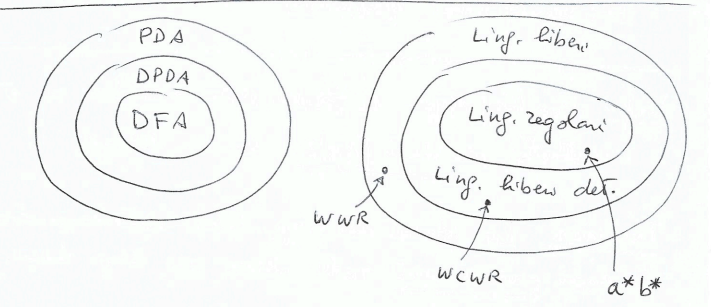
\includegraphics[width=10cm]{gerarchia_automi.png}
    %\end{center}
    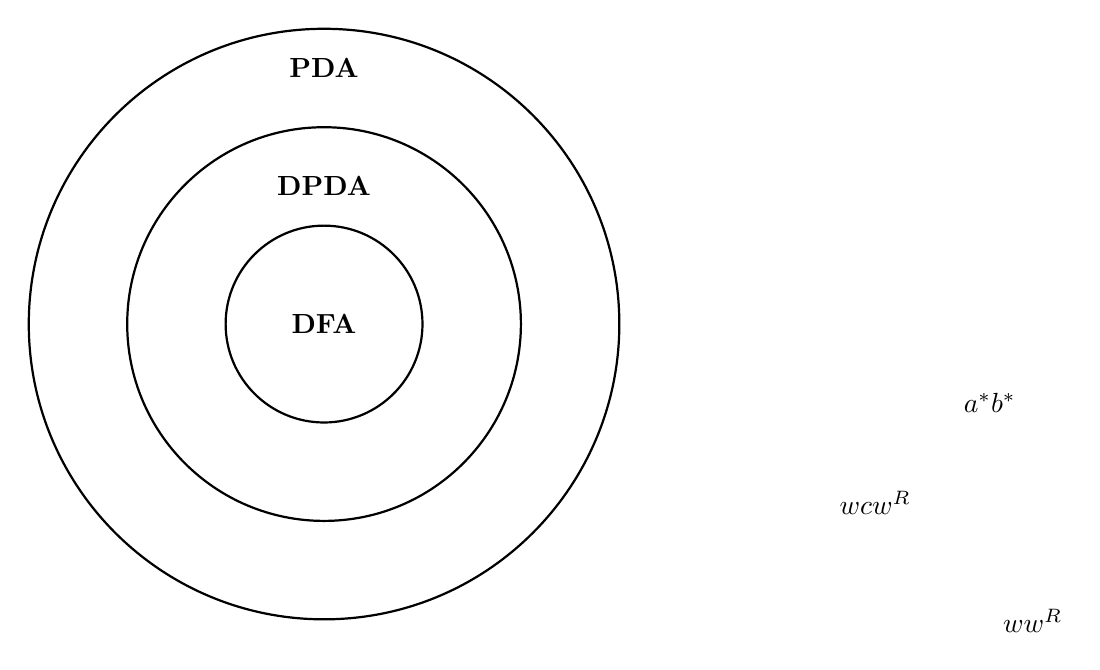
\begin{tikzpicture}
        % Cerchi per gli automi
        \draw[thick] (0, 0) circle (1.25cm) node[pos=0, yshift=0cm] {\textbf{DFA}};
        \draw[thick] (0, 0) circle (2.5cm) node[pos=0, yshift=1.75cm] {\textbf{DPDA}};
        \draw[thick] (0, 0) circle (3.75cm) node[pos=0, yshift=3.25cm] {\textbf{PDA}};
    
        % Cerchi per i linguaggi
        %\draw[thick] (8, 0) circle (1.5cm) node[pos=0, below right, xshift=-1.3cm] {\textbf{Linguaggi regolari}};
        %\draw[thick] (8, 0) circle (3cm) node[pos=0, above right, xshift=-2.1cm] {\textbf{Linguaggi liberi deterministici}};
        %\draw[thick] (8, 0) circle (4.5cm) node[pos=0, above right, xshift=-2.8cm] {\textbf{Linguaggi liberi}};
        
        % Annotazioni linguaggi
        \node[right] at (8, -1) {\(a^*b^*\)};
        \node[below] at (7, -2) {\(wcw^R\)};
        \node[below right] at (8.5, -3.5) {\(ww^R\)};
    \end{tikzpicture}
    
}
\pf{dimostrazione}{
    Se $L$ è regoalre, allora $\exists$ DFA $M$ tale che $L=L[M]$. A partire da $M$, posso costruire un DPDA $N$ si compore come $M$ senza mai manipolare lo stack, allora si che $L=L[N]$ per stato finale 
}
\subsubsection{Prefix propriety}
Si giunge così al seguente fatto:
\clm{}{}{
    Un linguaggio libero deterministico $L$ è riconosciuto da un $DPDA$ per pila vuota sse $L$ gode della "perfix propriety", ovvero 
    \[
        \nexists x,y\in L : x \text{ è prefisso di }y       
    \]
}
Pertanto si ha che:
\begin{itemize}
    \item Se $L$ è non gode della prefix propriety non può essere riconosciuto da un $PDPA$ per pila vuota
    \item Se $L$ è libero deterministico gode della prefix propriety, allora può essere riconosciuto da un $PDPA$ per pila vuota
    \item Se $L$ è libero deterministico, allora $L\$ =\{w\$ \mid w\in L\}$ gode della prefix propriety, infatti $L\$$ può essere riconosciuto da un $PDPA$ per pila vuota.
    
    Dove $\$\notin\Sigma$ ovvero $\$$ non è un simbolo dell'alfabeto di $L$, ma grazie ad esso alla fine di ogni linguaggio regolare vale la prefix propriety
\end{itemize}

\esempio{
    Sia $L_1 = \{a^nb^n\mid n\geq 0\}$ il seguente linguaggio che non gode della prefix propriety, in quanto $\epsilon\in L_1$ e $\epsilon$ è prefisso di $ab$

    \begin{tikzpicture}
        % States
        \node[state, initial, accepting] (q0) {\(q_0\)};
        \node[state, right of=q0] (q1) {\(q_1\)};
        \node[state, right of=q1] (q2) {\(q_2\)};
        \node[state, accepting, right of=q2] (q3) {\(q_3\)};
        
    
        % Transitions
        
        \draw (q0) edge[below] node {$\epsilon, Z/Z$} (q1);
        \draw (q1) edge[loop above] node[align=center] {$a,Z/AZ$} (q1);
        \draw (q1) edge[loop below] node[align=center] {$a,A/AA$} (q1);
        \draw (q1) edge[below] node {$b,A/\epsilon$} (q2);
        \draw (q2) edge[loop above] node[align=center] {$b,A/\epsilon$} (q2);
        \draw (q2) edge[below] node[align=center] {$\epsilon,Z/\epsilon$} (q3);
    
    \end{tikzpicture}
    
    Si ha quindi che il seguente linguaggio è riconosciuto da un DPDA \textit{per stato finale} e non \textit{per pila vuota}. Tuttavia il seguente linguaggio con il $\$\notin\Sigma$ è riconosciuto da un DPDA per \textit{per pila vuota}

    Sia $L_1\$$:


    \begin{tikzpicture}
        % States
        \node[state, initial] (q0) {\(q_0\)};
        \node[state, accepting, below of=q0] (q1) {\(q_1\)};
        \node[state, right of=q0] (q2) {\(q_2\)};
        \node[state, right of=q2] (q3) {\(q_3\)};
        
    
        % Transitions
        
        \draw (q0) edge[below] node {$a, Z/AZ$} (q2);
        \draw (q0) edge[left] node {$\$,Z/\epsilon$} (q1);
        \draw (q3) edge[loop above] node[align=center] {$b,A/\epsilon$} (q3);
        \draw (q3) edge[left] node[align=right] {$\$, Z/\epsilon$} (q1);
        \draw (q2) edge[loop above] node[align=center] {$a,A/AA$} (q2);
        \draw (q2) edge[below] node[align=center] {$b,A/\epsilon$} (q3);
    
    \end{tikzpicture}

    Si verifichi, infatti, come egli venga riconosciuto per pila vuota

}

\esempio{
    Sia $L_3 = \{a^nb^m\mid n\geq m \geq 0\}$ e dato che $\epsilon\in L_3$ tale linguaggio non gode della prefix propriety

    \begin{tikzpicture}
        \node[state, initial, accepting] (q0) {$q_0$};
        \node[state,  accepting, right of=q0] (q1) {$q_1$};
        \node[state,  accepting, right of=q1] (q2) {$q_2$};
        \node[state,  accepting, right of=q2] (q3) {$q_3$};

        \draw (q0) edge[above] node[align=center] {$a,Z/AZ$} (q1);
        \draw (q1) edge[above] node[align=center] {$b,A/\epsilon$} (q2);
        \draw (q2) edge[above] node[align=center] {$\epsilon, Z/\epsilon$} (q3);
        \draw (q2) edge[loop above] node[align=center] {$b,A/\epsilon$} (q2);
        \draw (q1) edge[loop above] node[align=center] {$b,A/AA$} (q1);
        
    \end{tikzpicture}

    e sia $L_3\$$:

    \begin{tikzpicture}
        \node[state, initial] (q0) {$q_0$};
        \node[state,  right of=q0] (q1) {$q_1$};
        \node[state,  right of=q1] (q2) {$q_2$};
        \node[state,  above of=q1] (q3) {$q_3$};
        \node[state,  below of=q1] (q4) {$q_4$};

        \draw (q0) edge[above] node[align=center] {$a,Z/AZ$} (q1);
        \draw (q0) edge[left] node[align=center] {$\$,Z/\epsilon$} (q3);
        \draw (q1) edge[above] node[align=center] {$b,A/\epsilon$} (q2);
        \draw (q1) edge[left] node[align=center] {$\$,A/\epsilon$} (q4);
        \draw (q2) edge[right] node[align=center] {$\$, Z/\epsilon$} (q3);
        \draw (q2) edge[right] node[align=center] {$\$, A/\epsilon$} (q4);

        \draw (q2) edge[loop right] node[align=center] {$b,A/\epsilon$} (q2);
        \draw (q1) edge[loop above] node[align=center] {$b,A/AA$} (q1);
        \draw (q4) edge[loop left] node[align=center] {$\epsilon,X/\epsilon$} (q4);

        
    \end{tikzpicture}


}

\subsubsection{non ambiguità dei linguaggi liberi deterministici}
\mprop{}{
    Se $L$ è libero deterministico, ovvero riconosciuto da un $DPDA$ per \textit{stato finale}, allora $L$ è generabile da una \textbf{grammatica libera non ambigua}.
    
    Si ha quindi che i \red{linguaggi liberi deterministici non sono ambigui}
}


%! errori e non capisco il motivo puercos zios
\subsubsection{Proprietà dei linguaggi liberi deterministici}

I lunguaggi liberi deterministici presentano le seguenti proprietà:
\mprop{chiusura solo per complementazione}{
    Sia $L$ un linguaggio libero deterministico, allora questo è chiuso per complementazione, ovvero:
\[
        (\exists \; \text{DPDA} \; N \; : \; L = L(N)) \implies (\exists \; \text{DPDA} \; N' \; : \; \overline{L} = L(N')) \quad \text{dove} \quad \overline{L} = \Sigma^* \setminus L
\]
}
\dimostrazione{
    Bisogna rendere totale la $\delta$ di $N$, eventualmente aggiungendo stati non finali, e poi $N'$ si ottiene da questo $N$ "aumentato", semplicemente scambiando \red{finali e non finali} 
}

\mprop{
    Non chiusura per intersezione
}{
    Un linguaggio libero deterministico non è chiuso per intersezione
}
\esempio{
    $L_1 =\{a^nb^nc^m\mid n,m\geq 0\}$ è libero deterministico\\
    $L_2 =\{a^mb^nc^n\mid n,m\geq 0\}$ è libero deterministico\\
    ma\\
    $L_1\cap L_2 =\{a^nb^nc^n\mid n\geq 0\}$ non è libero!

}

\mprop{
    non chiusura per unione
}{
    Un linguaggio libero deterministico non è chiuso per unione
}
\dimostrazione{
    Assumiamo per assurdo che un linguaggio libero deterministico sia chiuso per unione, allora:
    \[
        L_1\cap L_2 = \overline{\overline{L_1}\cup \overline{L_2}}    
    \]

    Per questo fatto e la proprosizione precedente si è verificato un assurdo
}

\subsection{Analizzatori sintattici: parser}
\begin{tikzpicture}[node distance=2cm]

        % Nodes
        \node (grammar) [startstop] {Grammatica Libera};
        \node (algorithm) [process, right of=grammar, xshift=4cm] {Algoritmo di \\ Costruzione (YACC)};
        \node (parser) [startstop, right of=algorithm, xshift=4cm] {Parser};
        \node (tokens) [startstop, below of=grammar, yshift=-2.5cm] {Lista di Token};
        \node (parser2) [process, right of=tokens, xshift=4cm] {Parser};
        \node (tree) [startstop, right of=parser2, xshift=4cm] {Albero di Derivazione};
        \node (additional) [below of=parser] {fondamentalmente un \\$DPDA$ con output};
        
        % Arrows
        \draw [arrow] (grammar) -- (algorithm);
        \draw [arrow] (algorithm) -- (parser);
        \draw [arrow] (tokens) -- (parser2);
        \draw [arrow] (parser2) -- (tree);
        \draw [wavearrow] (additional) -- (parser);
        
        % Additional text
        
        
        
        
\end{tikzpicture}

I parser possono essere:
\begin{itemize}
    \item \textbf{nondeterministici}: se, durante la ricerca di una derivazione, si scopre che una scelta è improduttiva e non porta a riconoscere l'input, \red{il parser torna indietro} (\textit{backtracking}), disfa parte della derivazione appena costruita e scegli un'altra produzione, \red{tornando a leggere parte dell'input}
    \item \textbf{deterministici}: leggono l'input una sola volta ed \red{ogni loro decisione è definitiva}
\end{itemize}

entrambi cercano di sfruttare informazioni dall'input per guidare la ricerca della derivazione

\subsubsection{introduzione al top-down parsing}
\dfn{}{
    Data $G=(NT,T,S,R)$ lebera, costruiamo il $PDA\;M=(T,\{q\}, T\cup NT, \delta, q, S, \varnothing)$, che riconosce per pila vuota, dove $\delta:Q\times(\Sigma\cup\{\epsilon\})\times\Gamma→Q\times\Gamma^*$ è definita:
    \begin{itemize}
        \item \textbf{espandi}: $(q,\beta)\in \delta(q,\epsilon, A)$ se $A\to\beta\in R$ 
        \item \textbf{consuma}: $\forall a\in T((q,\epsilon)\in \delta(q,a, a))$ 
    \end{itemize} 
    Tale che $L(G)=P[M]$ (riconoscimento per pila vuota)
}

Quindi, grazie alla prima regola se il simbolo in cima alla pila è un non terminale $A$, l'automa può espanderlo sostituendolo con la produzione $\beta$, come descritto nelle regole $R$ della grammatica, mentre secondo la regola di consumazione si ha che se il simbolo sulla cima della pila e il simbolo corrente della stringa in input sono entrambi a, allora l'automa può eliminare quel simbolo dalla pila e procedere nella lettura dell'input.

\esempio{
    Sia $G$ la seguente grammatica:
    \[
        \begin{array}{l}
            S\to aSb\mid \epsilon
        \end{array}    
    \]

    Si ha che $S\implies aSb \implies aaSbb \implies aabb$

    \begin{center}
       \begin{tikzpicture}
        \node[state] (q) {$q_0$};
        \draw (q) edge[loop right] node[align=center] {$b,b/\epsilon$} (q);
        \draw (q) edge[loop above] node[align=center] {$a,a/\epsilon$} (q);
        \draw (q) edge[loop left] node[align=center] {$\epsilon,S/\epsilon$} (q);
        \draw (q) edge[loop below] node[align=center] {$\epsilon,S/aSb$} (q);
    \end{tikzpicture} 
    \end{center}

    Si osservi che il seguente automa che riconosce il linguaggio della grammatica $S$ non è un PDPA

    Nella maggior parte delle configurazioni standard di un Pushdown Automaton (PDA) utilizzato per il parsing top-down, la pila viene inizializzata con il simbolo iniziale della grammatica, nel nostro caso, quindi, la serie di passaggi che porteranno a riconoscere il linguaggio sarà:
    \[
        \begin{array}{l}
            (q,aabb,S) \vdash (q,aabb,aSb)\\
            \vdash (q,abb,Sb)\vdash (q,abb,aSbb)\\
            \vdash  (q,bb,Sbb)\vdash (q,bb,bb)\\
            \vdash (q,b,b)\vdash (q,\epsilon,\epsilon)
        \end{array}
    \]
    che costruisce il seguente albero di derivazione 
    \begin{center}
        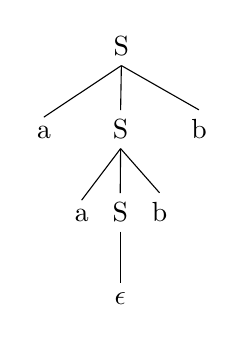
\begin{tikzpicture}
            \Tree [.S 
                        a
                        [.S
                            a
                            [.S
                                $\epsilon$
                            ]
                            b
                        ]
                        b
                ]
        \end{tikzpicture}
    \end{center} 

    Si ha, quindi:
    \begin{itemize}
        \item derivazione canonica a sx (leftmost)
        \item costruzione dell'albero dall'alto in basso
    \end{itemize}

    %TODO triangolo
}

Tuttavia in questo esempio è facile verificare che il parser è nondeterministico, infatti l'automa è un $PDA$, tuttavia questo nondeterminismo può essere risolto \red{scegliendo la produzione in baso al simbolo di lettura nell'input} (\textbf{look-ahead}), ad esempio:
\begin{itemize}
    \item se leggo $a$, espando $S\to aSb$
    \item se leggo $b$, espando $S\to \epsilon$
\end{itemize}

\begin{center}
  \begin{tabular}{rrr}
    \textbf{input} & \textbf{stack}&\textbf{azione}\\
    $\underline{a}abb\$$&$S$&leggo $a$ e espando in $aSb$ \\
    & $\underline{a}Sb$&consumo\\
    $\underline{a}bb\$$&$Sb$&leggo $a$ e espando in $aSb$\\
    &$\underline{a}Sbb$&conumo\\
    $\underline{b}b\$$ & $Sbb$&leggo $b$ e espando in $\epsilon$\\
    &$\underline{b}b$&consumo\\
    $b\$$&$b$&leggo $b$ e espando in $\epsilon$ \\
    $\$$ & $\epsilon$& fin
\end{tabular}  
\end{center}

\nt{
    Non tutte le grammatiche sono adatte per il top down-parser
}
\esempio{
    Sia $G$ la segnuete grammatica:
    \[
        S\to Sb\mid a        
    \]
    e $L(G)=ab^*$ (linguaggio regolare semplice)

    L'automa che riconosce il linguaggio è:
    \begin{center}
        \begin{tikzpicture}
         \node[state] (q) {$q$};
         \draw (q) edge[loop right] node[align=center] {$b,b/\epsilon$} (q);
         \draw (q) edge[loop above] node[align=center] {$a,a/\epsilon$} (q);
         \draw (q) edge[loop left] node[align=center] {$\epsilon,S/a$} (q);
         \draw (q) edge[loop below] node[align=center] {$\epsilon,S/Sb$} (q);
     \end{tikzpicture} 
     \end{center}

     Con i seguenti passaggi:
     \[
        (q,ab,S)\vdash(q,ab,Sb)\vdash(q,ab,Sbb)\vdash\dots   
     \]
     Qui il determinismo non funziona, infatti se vogliamo espandere quando leggiamo $a$ in input non possiamo anche consumare, pertnato l'automa espanderà all'infinito

     Occorre manipolare la grammatica affinche non vi siano ricorsioni sinistre
}

\subsubsection{
    Introduzione al botto-up parsing
}
\clm{}{}{
    Data una grammatica libera $G = (NT, T, R, S)$, costruiamo un $PDPA\;M = (T,\{q\},T\cup NT\cup\{Z\},\delta,q,Z,\varnothing)$ che riconosce $L(G).\$$ dove:
    \begin{itemize}
        \item \textbf{shift}: $\forall a \in T,\Big(\forall X\in T\cup NT\cup Z,\big((q,aX)\in \delta(q,a,Z)\big)\Big)$
        \item \textbf{reduce}: $(A\to\alpha R)\implies(q,A)\in\delta (q,\epsilon,\alpha^R)$ 
        
        Con $\alpha^R$ una generalizzazione dei $PDA$ in cui si consuma una stringa sulla pila anziché solo il top
        \item \textbf{accept}: \((q,\epsilon)\in \delta (q,\$,SZ)\)
        
        Con $S$ che deve essere alla fine sulla pila e $\$$ simbolo di fine input
    \end{itemize}
}

Cominciamo subito con un esempio
\esempio{
    Sia $G$ la seguente grammatica:
    \[S\to aSb\mid ab\]

    
\begin{center}
    \begin{tikzpicture}
        \node[state] (q) {$q$};
        
        \draw (q) edge[loop above] node[align=center] {$a,a/\epsilon$} (q);
        \draw (q) edge[loop right] node[align=center] {$b,b/\epsilon$} (q);
        \draw (q) edge[out=330, in=300, looseness=8] node[align=center] {$c,c/\epsilon$} (q);
        \draw (q) edge[out=210, in=240, looseness=8] node[align=center] {$d,d/\epsilon$} (q);
        \draw (q) edge[loop left] node[align=center] {$e,e/\epsilon$} (q);
    \end{tikzpicture}
\end{center}

\begin{center}
    \begin{tabular}{lll}
        \textbf{stack}&\textbf{input}&\textbf{azione}\\
        $Z$ & $aabb\$$ & shift\\
        $Za$ & $abb\$$ & shift\\
        $Zaa$ & $bb\$$ & shift\\
        $Zaab$ & $b\$$ & reduce $S\to ab$\\
        $ZaS$&$b\$$ & shift \\
        $ZaSb$ & $\$$ & reduce $S\to aSb$\\
        $ZS$ & $\$$ & \textit{accept}\\
        $\epsilon$ & $\epsilon$ &
    \end{tabular}
\end{center}

In passaggi, $S\implies aSb \implies aabb$. Viene prodotto il seguente albero di derivazione:

\begin{center}
    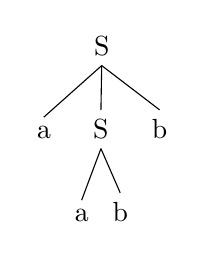
\begin{tikzpicture}
    \Tree[.S 
        a
        [.S
            a
            b
        ]
        b
    ]
    \end{tikzpicture}    
\end{center}

Si può verificare come come la costruzione dell'input sia:
\begin{itemize}
    \item \textbf{left-to-right} (come leggo l'input)
    \item \textbf{right-derivatione}
    \item 
\end{itemize}

Tuttavia  è facile verificare che c'è molto nondeterminismo:
\begin{itemize}
    \item Conflitti: Shift-Reduce
    \begin{enumerate}
        \item $zaab \quad b\$ \quad$ (può fare shift)
        \item $zaabb \quad \$ \quad$ (ma è un percorso infruttuoso)
    \end{enumerate}
    \item Conflitti: Reduce-Reduce
    
    Più riduzioni possibili (non ci sono in quest'esempio, ma con grammatiche più complesse è possibile)

\end{itemize}
}

Per ottenere un DPDA, serve introdurre informazioni aggiuntive per risolvere i conflitti:
\begin{itemize}
    \item \textbf{Più stati:} (o strutture particolari di supporto alle decisioni, come un DFA dei prefissi validi).
    \item \textbf{Look-ahead:} (guardare l'input in avanti).
\end{itemize}

Vediamo un esempio più corposo relativo alle grammatiche delle espressioni aritmetiche:

\esempio{
    Sia $G$ tale grammatica:
    \[
        \begin{aligned}
            & E \to T + E \mid T \\
            & T \to T \times A \mid A \\
            & A \to a \mid b \mid (E)
        \end{aligned}
    \]
    Si ha:

    %! modificare il reduce
    \[
        \begin{array}{|c|l|}
        \hline
        \textbf{G} & \textbf{M} \\
        \hline
        & t_0 : \delta(q, a, X) = (q, aX) \; \forall aX \quad \text{SHIFT} \\
        \text{(R1)} \; E \to T + E  & t_1 : \delta(q, \epsilon, E + T) = (q, E) \\
         \text{(R2)} \; E \to T & t_2 : \delta(q, \epsilon, T) = (q, E) \\
        \text{(R3)} \; T \to T \ast A & t_3 : \delta(q, \epsilon, A \ast T) = (q, T) \quad \text{REDUCE} \\
        \text{(R4)} \; T \to A & t_4 : \delta(q, \epsilon, A) = (q, T) \\
        \text{(R5)} \; A \to (E) & t_5 : \delta(q, \epsilon, (E)) = (q, A) \\
        \text{(R6)} \; A \to a & t_6 : \delta(q, \epsilon, a) = (q, A) \\
        \text{(R7)} \; A \to b & t_7 : \delta(q, \epsilon, b) = (q, A) \\
                            & t_8 : \delta(q, \$, EZ) = (q, \epsilon) \quad \text{ACCEPT} \\
        \hline
        \end{array}
    \]
    La cui sequenza è:
    \[
        a*(b)\Leftarrow A*(b) \Leftarrow T*(b)\Leftarrow T*(A) \Leftarrow T*(T)\Leftarrow T*(E)\Leftarrow T*A \Leftarrow T \Leftarrow E
    \]

    La cui pila-stack-input è:
    \[
        \begin{array}{|c|c|c|}
            \hline
            \textbf{Stack} & \textbf{Input} & \textbf{Action} \\
            \hline
            Z & a \ast (b) \$ & \text{shift} \\
            Z a & \ast (b) \$ & \text{reduce } R_6 \\
            Z A & \ast (b) \$ & \text{reduce } R_4 \\
            Z T & \ast (b) \$ & \text{shift} \\
            Z T \ast & (b) \$ & \text{shift} \\
            Z T \ast ( & b) \$ & \text{shift} \\
            Z T \ast ( b & ) \$ & \text{shift} \\
            Z T \ast ( b ) & \$ & \text{reduce } R_7 \\
            Z T \ast ( A & ) \$ & \text{reduce } R_4 \\
            Z T \ast ( T & ) \$ & \text{reduce } R_2 \\
            Z T \ast ( E & ) \$ & \text{shift} \\
            Z T \ast ( E ) & \$ & \text{reduce } R_5 \\
            Z T \ast A & \$ & \text{reduce } R_3 \\
            Z T & \$ & \text{reduce } R_2 \\
            Z E & \$ & \text{accept} \\
            \epsilon &\epsilon & \\
            \hline
        \end{array}
    \]

    Il cui albero di derivazione:
    \begin{center}
        \begin{tikzpicture}
        \Tree[.E 
            [.T
                [.T
                    [
                        .A
                        [
                            .a
                        ]
                    ]
                ]
                *
                [
                    .A
                    $($
                    [
                        .E
                        [
                            .T
                            [
                                .A
                                [
                                    .b
                                ]
                            ]
                        ]
                    ]
                    $)$
                ]
            ]
        ]
        \end{tikzpicture}    
    \end{center}



}

L'automa è non deterministico perché:
\begin{enumerate}
    \item Chi ha precedenza tra \textit{shift} e \textit{reduce}?
    
    \textbf{Ad esempio:}
    \begin{enumerate}
        \item[1)] $Z a \quad * \, (b) \, \$ \quad$ \textit{shift}
        \item[2)] $Z a * \quad (b) \, \$ \quad$ non buono! Qui \textit{reduce} è in conflitto con \textit{shift}!
    \end{enumerate}
    
    \textbf{Altro esempio:}
    \begin{enumerate}
        \item $Z T \quad * \, (b) \, \$ \quad$ \textit{reduce } $R_2$
        \item $Z E \quad * \, (b) \, \$ \quad$ non buono! Qui \textit{shift} è in conflitto con \textit{reduce}!
    \end{enumerate}
    
    \item Chi ha precedenza tra due diverse \textit{reduce}?
    
    \textbf{Ad esempio:}
    \begin{enumerate}
        \item $Z T * A \quad \$ \quad$ \textit{reduce } $R_3$
        \item $Z T \quad \$$
        \item $Z T * T \quad \$ \quad$ se faccio, \textit{reduce } $R_4$ \\
        Qui \textit{reduce} $R_3$ è in conflitto con \textit{reduce} $R_4$!
    \end{enumerate}
    
    È buona norma scegliere in modo tale che ciò che si trova nella pila sia un prefisso (a rovescio) di una parte destra di una produzione della grammatica.
    
    \textbf{Ad esempio:}
    \begin{enumerate}
        \item $Z a$
        \item $Z A$ con la ``norma'' produco chi coincide con ciò che è un prefisso di una parte destra che comincia con $A$.
    \end{enumerate}
\end{enumerate}

\subsubsection{problema con le pruzioni $\epsilon$}
Sia la produzione $S\to \epsilon$

TODO! NON HO CAPITO


\section{Semplificazione delle grammatiche}
Per avere \textbf{PDA} efficienti e con minor non determinismo è necessario semplificare le grammatiche. Ad esempio:
\begin{itemize}
    \item Eliminare le produzioni $\epsilon$ (del tipo $A\to\epsilon$) inadatte al bottom up parsing
    \item Eliminare le \red{produzione unitarie} (del tipo $A\to B$ che possono creare dei cicli $A \implies^+ A$) 
    \item Eliminare \red{simboli inutili}, cioè quei terminali e non terminali che non sono raggiungibili/generabili a partire dal simbolo inziale $S$
    
    es. gli stati d'errore 

    \item  Eleminare \red{la ricorsione sinistra} (del tipo $A \to A\alpha$), perché inadatte al top - down parsing
    \item \red{fattorizzare} le grammatiche, per ottenere grammatiche con meno non determinismo nel top-down parsing
\end{itemize}

\subsection{Eliminare le produzioni $\epsilon$}
Per fare ciò si usi un algoritmo che ha:
\begin{itemize}
    \item in \red{input}: una $G$ libera con produzione $\epsilon$ 
    \item in \red{output}: una $G'$ libera senza produzione $\epsilon$ tale che $L(G') = L(G)\backslash\{\epsilon\}$ 
\end{itemize}

\osservazione{
    Se $\epsilon \in L(G)$ e si vuole ottenere una $G''$ t.c. $L(G)= L(G'')$, basta considerare $G' = (NT,T,S,R')$ e definire $G'' = G' \cup \{S' \to \epsilon | S\}$ t.c.
    \[
        G'' = (NT\cup\{S'\},T,S',R'\cup \{S' \to \epsilon|S\})
    \]
}
\subsubsection{simboli annullabili}
Per l'algoritmo occorre innanzi tutto definire i \textbf{simboli annullabili}
\dfn{simboli annullabili}{ \label{semplificazioneGram}
    I \textbf{simboli annullabili} sono quei non terminali tale che possono riscriversi in uno o più passi in $\epsilon$, ovvero:
    \[
        N(G) = \{A\in NT | A \implies^{+} \epsilon\}    
    \]
    Dove $N(G)$ è l'insieme dei simboli annullabili e viene calcolato induttivamente come segue:
    \begin{itemize}
        \item $N_0 (G) = \{A\in NT | A\to \epsilon \}$, questo è il caso in cui un non terminale $A$ viene riscritto direttamente in $\epsilon$ tramite una produzione
        \item $N_{i+1}(G) = N_i (G) \cup\{B\in NT | B \to c_1,\dots, c_k \in \mathbb{R}\text{ e } c_1,\dots, c_k \in N_i(G)\}$ questo è il caso in cui un non terminale $B$ possa essere ricondotto a a $\epsilon$ in più passi
    \end{itemize}
}

Ovviamente $\exists i_c$ tale che $N_{i_c}(G)=N_{i_c+1}(G)$, cioè che ad un certo punto non aggiungo nessun altro $B$ all'insieme ($NT$ è finito)
\teorema{
    L'insieme $N(G) = N_{i_c}(G)$ è esattamente l'insieme di tutti i simboli annullabili
}

\subsubsection{algoritmo per il calcolo della grammatica}


Una volta calcolato \( N(G) \) per \( G = (N, T, S, R) \), costruiamo la grammatica \( G' = (N, T, S, R') \) dove per ogni produzione \( A \rightarrow \alpha \in R \) con \( \epsilon \not\in \alpha \), in cui occorrono simboli annullabili \( Z_1, \ldots, Z_k \), mettiamo in \( R' \) tutte le produzioni del tipo \( A \rightarrow \alpha' \) dove \( \alpha' \) si ottiene da \( \alpha \) cancellando tutti i possibili sottoinsiemi di \( Z_1, \ldots, Z_k \) (incluso \( \varnothing \)), ad eccezione del caso in cui \( \alpha' \) risulta \( \epsilon \), in altre parole si creano tutte le possibili combinazioni di $\alpha$ eliminando uno o più di questi simboli $Z_1,\dots,Z_n$:

\begin{itemize}
    \item in \( G' \) non mettiamo produzioni \( A \rightarrow \epsilon \in R \),
    \item in \( G' \) non introduciamo mai produzioni del tipo \( A \rightarrow \epsilon \).
\end{itemize}

\teorema{
    Data una grammatica libera \( G \), la grammatica \( G' \) determinata dall'algoritmo sopra non ha \( \epsilon \)-produzioni, e \( L(G') = L(G) \setminus \{\epsilon\} \)
}

\esempio{
    Sia $G$ una grammatica tale che:
    \[
        G = \begin{cases}
            S \to AB \\
            A\to aAA\mid\epsilon\\
            B\to bBB\mid\epsilon
        \end{cases}    
        \quad
        N_0(G)=\{A,B\} \text{ e }N_1(G)=\{A,B,S\} = N(G)
    \]
    Quindi tutti sono simboli annullabili

    Adesso procedo con l'algoritmo, procedo per ogni simbolo annullabili
    \begin{itemize}
        \item $S\to AB$: secondo l'algoritmo devo cancellare in tutti i modi possibili i simboli non terminali che compaiono nella parte destra della produzione. In questo caso dobbiamo considerare 4 casi:
        \begin{itemize}
            \item $\emptyset\implies S\to AB$, rinuncio a cancellare
            \item $\{B\}\implies S\to A$, se cancello $B$ rimane $A $nella parte destra
            \item $\{A\}\implies S\to B$
            \item $\{A,B\}\implies S\to \epsilon$ dato che non devo mai introdurre produzioni del tipo \( A \rightarrow \epsilon \) \red{non posso cancellare $A$ e $B$}
        \end{itemize}
        Unisco i vari sottoinsiemi e si ha:
        \[
            S\to AB|B|A
        \]
        \item $A\to aAA\in R$. dobbiamo considerare 4 casi:
        \begin{itemize}
            \item $\emptyset\implies A\to aAA$
            \item $\{A\}\implies A\to aA$
            \item $\{A,A\}\implies A\to a$
        \end{itemize}
        Quindi si ha:
        \[
            A\to aAA|aA|a    
        \]
        \item si ha la stessa cosa con $B$, quindi cancellarehe verrà trasformato in 
        \[
            B\to bBB|bB|b    
        \]
        Così la nuova grammatica sarà:
        \[
            G' = \begin{cases}
                S\to AB|A|B\\
                A\to aAA|aA|a\\
                B\to bBB|bB|b
            \end{cases}    
        \]
    \end{itemize}
}
\subsection{Eliminazione delle produzioni unitarie}


\dfn{Produzione unitaria}{
    Una produzione si dice \textbf{unitaria} quando $A\to B$ si ha che $A,B\in NT$
}

\subsubsection{coppie unitarie}
Per eliminare queste produzioni unitarie si deve però calcolare quelle che sono definite le "coppie unitarie"
\dfn{Coppia unitaria}{
    Una coppia $(A,B)$ si dice \textbf{unitaria} qunado $A\implies^* B$ (quindi quando $A$ può riscriversi in 0 o più passi nel non terminale $B$) usando solo produzioni unitarie. 
    
    Vi è qui ripostata la definizione induttiva:
    \begin{itemize}
        \item $U_0(G) = \{(A,A)|A\in NT\}$, quindi ogni non terminale fa coppia con se stesso
        \item $U_{i+1}(G) = U_i (G)\cup \{(A,C)|(A,B)\in U_i(G)\}$ e $B\to C\in R$, quindi è l'insieme delle coppie al passo $i$ unito alle coppie alle coppie $(A,C)$ tali che $(A,B)$ sono coppie presenti nell'insieme dell'iterazione precedente e $B\to C \in R$
    \end{itemize} 
}

Anche in questo caso $\exists i_c$ t.c. $U_{i_c}(G) = U_{i_c+1}(G)$ dato che $NT$ è finito. Pertanto per definizione si ha che $U(G) = U_{i_c}(G)$, detto insieme di tutte le coppie unitarie

\subsubsection{algoritmo per il calcolo dell'eliminazione delle produzioni unitarie}

Data $G = (N, T, R, S)$ libera, si definisce una $G' = (N, T, R', S)$ dove, per ogni $(A, B) \in U(G)$, $R'$ contiene 
tutte le produzioni $A \rightarrow \alpha$, dove $B \rightarrow \alpha \in R$ 
e non è unitaria

\osservazione{
    Poiché, per ogni $A \in N$, la coppia $(A, A) \in U(G)$, $R'$ contiene tutte le produzioni non unitarie di $R$ e in aggiunta un po' di altre.
}

\teorema{
    Sia $G = (NT, T , R, S)$ libera e sia $U(G)$ l'insieme selle sue coppie unitarie. Sia $G' = (NT, T, R', S)$ la grammatica ottenuro dall'algoritmo $G'$ non ha produzione unitarie e $L(G) =  L (G')$
}

Esempietto:
\esempio{
    Prediamo con esempio la grammatica non ambigua $E$ delle espressioni aritmetiche:
    \[
        E = \begin{cases}
            E\to E+ T|T\\
            T\to T * A|A\\
            A\to a|b|(E)
        \end{cases}       
    \]
    Si noti subito che ha 2 produzioni unitarie: $E\to T \text{ e }T\to A$.
    Iniziamo a calcolare l'insieme delle coppie unitarie:
    \begin{itemize}
        \item $U_0(G) = \{(E,E),(T,T),(A,A)\}$ e grazie al cuzzo
        \item $U_1(G) =U_0(G) \cup \{(E,T),(T,A)\}$
        \item $U_2(G) =U_1(G) \cup \{(E,A)\} = U_3(G) = U(G)$ dato che da che da $E$ si arriva ad $T$ e si arriva $A$
    \end{itemize}

    Per calcolare la grammatica $G'$ devo prendere tutte le produzioni non unitarie della grammatica originale, ovvero: 
    \[
        G' = \begin{cases}
            E\to E+T\\
            T\to T\times A\\
            A\to a|b|(E)
        \end{cases}
    \]
    In aggiunta:
    \[
        \begin{cases}
            E\to E+T  & \text{ perché } (E,T)\in U_1(G)\\
            T\to a|b|(E) & \text{ perché } (T,A)\in U_1(G)\\
            E\to a|b|(E) & \text{ perché } (E,A)\in U_2(G)
        \end{cases}
    \]
    Pertanto $G'$ sarà:
    \[
        G' = \begin{cases}
            E\to E+T | T\times A|a|b|(E)\\
            T\to T\times A|a|b|(E) \\
            A\to a | b | (E)
        \end{cases}    
    \]

    Sia ha che non contiene produzioni unitarie ed è equivalente a $G$
}
\subsection{Rimuovere i simboli inutili}

\dfn{Simboli generatori, raggiungibili e utili}{
    Un simbolo $X\in T\cup NT$ è 
    \begin{itemize}
        \item Un \red{generatore} $\iff \exists w \in T^*$ con $x\implies^* w$ 
        
        Quindi un generatore è o un terminale (un simbolo può riscriversi in se stesso) oppure un non terminale che in uno o più passi. è definito induttivamente come segue:
        \begin{itemize}
            \item $G_0(G)= T$ se $a\in T, a\implies^* a$ (quindi tutti i terminali sono generatori)
            \item $G_{i+1}(G)= G_i(G)\cup \{B\in NT|B \to C_1,\dots C_k \in R \land C_1,\dots, C_k \in G_i(G)\}$
        \end{itemize}
        \item Un \red{raggiungibile} $\iff (\exists\alpha,\beta \in (T\cup NT)^*.( S\implies^*\alpha X \beta))$. Sono definiti induttivamente:
        \begin{itemize}
            \item $R_0(G) = \{S\}$
            \item $R_{i+1}(G) = R_i(G)\cup\{x_1, \dots, x_k\} \forall B\in R_i (G), B\to x_i,\dots, x_k \in R$ 
        \end{itemize}
        \item \red{utile} sse è sia un generatore e sia raggiungibile, ovvero se $S\implies^* \alpha X \beta\implies^* x\in L(G)$ cioè $X$ compare in almeno una derivazione di una stringa $z\in L(G)$
    \end{itemize}
}


\subsubsection{algoritmo per l'eliminazione dei simboli inutili}
\begin{enumerate}
    \item Prima di tutto elimino tutti i non-generatori (e tutte le produzione che usano almeno uno di questi)
    \item Poi dalla nuova grammatica, elimino tutti i non - raggiungibili (E tutte le produzioni che li usano)
\end{enumerate}

\teorema{
    Sia $G=(NT,T,R,S)$ una grammatica libera t.c. $L(G) \neq \emptyset$
    \begin{itemize}
        \item Sia $G_1$ la grammatica che si ottiene da $G$ eliminando tutti i simboli che non a appartengono a $G(G)$ (insieme dei generatori), e tutte le produzioni che fanno uso di algoritmo di tali simboli
        \item Sia $G_2$ la grammatica che si ottiene da $G_1$ eliminando tutti i simboli che non appartengono a $R(G)$, e tutte le produzioni che fanno uso di almeno uno di tali simboli 
    \end{itemize}
    
    Allora $G_2$ non ha simboli inutili e $L(G_2) = L(G)$
}
\dimostrazione{
     La dimostrazione si divide nelle due parti dell'enunciato:
     \begin{itemize}
        \item $L(G_2 )\subseteq L (G)$ è ovvio, dato che $G_2$ contiene meno produzioni di $G$
        \item $L(G)\subseteq L(G_2)$: dobbiamo dimostrare che $S\implies^*_G w$ (ovvero se $S$ deriva $W$ usando le produzioni di $w$) allora $S\implies^*_{G_2 }w$
        
        Si ha che ogni simbolo usato in $S\implies^*_G w$ è, ovviamente, sia raggiungibile sia generatore

        Quindi quelle derivazioni è anche una derivazione per $G_2$

        Q.e.d.
     \end{itemize}
}

\osservazione{
    L'ordine dei due generatori è importante! 
    \begin{itemize}
        \item prima elimino i non-generatori
        \item poi i non - raggiungibili
    \end{itemize}
    ma se inverto l'ordine, allora può capitare che non elimino tutti i simboli inutili
}


Esempietto di eliminazione di tutti quei simboli non utili (inutili)

\esempio{
    Si parta da questa grammatica:
    \[
        G = \begin{cases}
            S \to AB|a \\
            B\to b
        \end{cases}       
    \]
    Poiché $a\implies^*a, b\implies^*b, S\implies^*a, B\implies^*b$ si ha che i generatori saranno $\{S,B,a,b\}$ (dove manca $A$). Possiamo così eleminare tutte le produzioni che includono $A$:
    \[
        G' = \begin{cases}
            S\to a\\
            B\to b
        \end{cases}    
    \]
    Adesso posso eliminare tutti i non raggiungibili da $S$, che in questo caso l'unico è solo $B$. Si ha che:
    \[
        G'' = S\to a    
    \]
    Si ha che $G''$è equivalente a $G$, ma non contiene simboli utili 
}

Esempio secondo:
\esempio{
    \[
        \begin{array}{l}
        G = 
        \begin{cases}
        S \rightarrow aC \\
        A \rightarrow a \\
        B \rightarrow bB \\
        C \rightarrow b \mid AC \\
        D \rightarrow a \mid aS
        \end{cases}
        \end{array}
    \]

    Poiché \( G(G) = \{ S, a, C, b, A, D \} \) e solo \( B \) non è generatore, possiamo eliminare tutte le produzioni che includono \( B \). Si ha quindi:

    \[
        \begin{array}{l}
        G_1 = 
        \begin{cases}
        S \rightarrow aC \\
        A \rightarrow a \\
        C \rightarrow b \mid AC \\
        D \rightarrow a \mid aS
        \end{cases}
        \end{array}
    \]

    A questo punto, notiamo che solo \( D \) non è raggiungibile, quindi possiamo eliminarlo. Si ottiene:

    \[
        \begin{array}{l}
        G_2 = 
        \begin{cases}
        S \rightarrow aC \\
        A \rightarrow a \\
        C \rightarrow b \mid AC
        \end{cases}
        \end{array}
    \]

    $G_2$ è la grammatica semplificata, equivalente a $G$, senza simboli inutili.
}
In questo esempio si ha che $L(G_2) = \{ab,aab,aaab,\dots\} = a^+b$

Si osservi però che è possibile trovare una grammatica più semplice per il linguaggio $a^+ b$:
\[
        S\to aS | ab
\]
\subsection{mettere insieme le cose}
Se, nel semplificare la grammatica $G$, \red{seguiamo questo ordine}:
\begin{itemize}
    \item Eliminare le $\epsilon\text{-produzioni}$
    \item Eliminare le produzioni unitarie (ovvero i cicli)
    \item eliminare i simboli inutili
\end{itemize}
allora la grammatica risultante \red{è garantita non avere nè $\epsilon\text{-produzioni}$, ne produzioni unitarie, ne simboli inutili ed è equivalente a quella di partenza}. 

\osservazione{
    Si presti attenzione all'ordine poiché alcune delle costruzioni possono interagire tra di loro


    durante la fase di eliminazione delle $\epsilon\text{-produzioni}$, potremmo introdurre produzioni unitarie, pertanto le $\epsilon\text{-produzioni}$ vanno eliminate prima della fase di eliminazione delle produzioni unitarie
}
Esempietto:
\esempio{
    \[
G = 
\begin{cases}
S \rightarrow a A a \mid a a \\
A \rightarrow C \\
C \rightarrow S \mid \varepsilon
\end{cases}
\]

\begin{enumerate}
    \item \textbf{Togliere le $\varepsilon$-produzioni}

    \[
    N(G) = \{ S, C, A \} \Rightarrow G' = 
    \begin{cases}
    S \rightarrow a A a \mid a a \\
    A \rightarrow C \\
    C \rightarrow S
    \end{cases}
    \]

    \item \textbf{Togliere le produzioni unitarie}

    \[
    U(G') = \{ (A, A), (C, C), (S, S), (A, C), (C, S), (A, S) \}
    \]
    
    \[
    G'' = 
    \begin{cases}
    S \rightarrow a A a \mid a a & \text{perché } (S, S) \in U(G') \\
    C \rightarrow a A a \mid a a & \text{perché } (C, S) \in U(G') \\
    A \rightarrow a A a \mid a a & \text{perché } (A, S) \in U(G')
    \end{cases}
    \]

    \item \textbf{Rimuovere i simboli inutili}

    \[
    G(G'') = \{ S, a, A, C \} \quad \text{tutti i generatori}
    \]
    \[
    R(G'') = \{ S, a, A \} \quad \text{ma non } C
    \]
    
    \[
    G''' = 
    \begin{cases}
    S \rightarrow a A a \mid a a \\
    A \rightarrow a A a \mid a a
    \end{cases}
    \]
\end{enumerate}


}

In questo esempio si ha che $L(G''') = \{aa,aaaa, \dots\} = (aa)^+$

Si osservi però che è possibile trovare una grammatica più semplice per il linguaggio $ (aa)^+$:
\[
        S\to aSa | aa 
\]
o anche 
\[
    S\to aaS|aa    
\]

\subsection{forme normali}
le \textbf{forme normali} sono particolari configurazioni di rappresentazione di un linguaggio formale o di un'espressione logica che rispettano determinate regole e strutture. Ne studieremo di due tipi:
\begin{itemize}
    \item \textbf{Chomsky}: Una grammatica è in forma normale di Chomsky se ogni produzione ha la forma $A\to BC$ o $A\to a$, dove $A, B,C\in NT$ e $a\in T$. Ogni produzione deriva quindi o una coppia di variabili o un singolo terminale. Questa forma è utile, per esempio, negli algoritmi di parsing
    \item \textbf{Greibach}: Una grammatica è in forma normale di Greibach se ogni produzione ha la forma $A\to a\alpha$, dove $A\in NT$, $a\in T$ e $\alpha$ è (eventualmente) una stringa di variabili. La GNF è usata in particolare per costruire parser discendenti
\end{itemize}
\subsubsection{Forma normale di Chomsky}
\dfn{Forma normale di Chomsky}{
    Una grammatica si dice in \textbf{forma normale di Chomsky} se sono nella forma:
    \[ 
        \begin{array}{l}
            A\to BC\\
            A\to a   
        \end{array}
    \] 
    Dove $\epsilon$ è trattato a parte $S\to \epsilon|BC$ e $S$ non compare mai a destra in una produzione 
}
\osservazione{
    se $G$ è libera in forma normale di Chomsky, allora:
    \begin{itemize}
        \item non ha $\epsilon\text{-produzioni}$
        \item non ha produzioni unitarie
    \end{itemize}
}

\osservazione{
    ogni grammatica libera $G$ può essere trasformata in una equivalente $G'$ in forma normale di Chomsky
}
\subsubsection{Forma normale di Greibach}
\dfn{forma normale di Greibach}{
    Una grammatica si dice in \textbf{forma normale di Greibach} se sono nella forma:
    \[ 
        \begin{array}{l}
            A\to aBC\\
            A\to aB \\
            A\to a   
        \end{array}
    \] 
    Dove $\epsilon$ è trattato a parte $S\to \epsilon|BC$ e $S$ non compare mai a destra in una produzione
}
\osservazione{
    se $G$ è libera in forma normale di Greibach, allora:
    \begin{itemize}
        \item non ha $\epsilon\text{-produzioni}$
        \item non ha produzioni unitarie
        \item non è ricorsiva a sinistra
        \item ogni produzione applicata in una derivazione allunga il prefisso di terminali $\implies$ il parser costruito a partire della forma normale di Greibach sono meno non deterministici
    \end{itemize}
}
\osservazione{
    ogni grammatica libera $G$ può essere trasformata in una equivalente $G'$ in forma normale di Greibach
}
\subsection{Eliminare la ricorsione a sinistra}
L'eliminazione della ricorsione a sinistra è un problema tipico dei parser top-down
\dfn{produzione ricorsiva a sinistra}{
    Si definisce \textbf{una produzione ricorsiva a sinistra} una produzione del tipo
    \[
        A\to A\alpha \in R    
    \]
}
\dfn{grammatica ricorsiva a sinistra}{
    Si definisce una \textbf{grammatica ricorsiva a sinistra} una grammatica $G$ del tipo:
    \[
        A\implies^+ A\alpha \text{ per qualche }A\in NT, \alpha \in (T\cup NT)^*       
    \]
}

Una tipica ricorsione a sinistra è: 
\[
    A\to A_{\alpha_1}|\dots|A_{\alpha_n} | \beta_1|\dots|\beta_n    
\]
Dove le stringhe $\beta_i$ non cominciano per $A$. Queste produzioni possono essere rimpiazzate da
\[
    \begin{array}{l}
        A\to \beta_1A'|\dots|\beta_m A'\\
        A'\to \alpha_1 A'|\dots|\alpha_n A'|\epsilon
    \end{array}    
\]
Se nella grammatica originale avviamo la derivazione 
\[
    A\implies A\alpha_{i_1} \implies A\alpha_{i_2}\alpha_{i_1} \implies\dots\implies A\alpha_{i_k}\dots\alpha_{i_2}\alpha_{i_1} \implies \beta_i \alpha_{i_k}\dots\alpha_{i_2}\alpha_{i_1}
\]
Con la nuova grammatica si ha:
\[
    A\implies\beta_iA'\implies \beta_i \alpha_{i_k} A' \implies\dots\implies\beta_i\alpha_{i_k}\dots\alpha_{i_2}A'\implies\beta_i\alpha_{i_k}\dots\alpha_{i_1}A'\implies\beta_i\alpha_{i_k}\dots\alpha_{i_1}
\]

Esempi concreti:
\esempio{
    \[
        \begin{array}{l}
            A\to Aa|b \\
            \Rightarrow\\
            A\to bA'\\
            A' \to aA'|\epsilon    
        \end{array}
    \]
    Poi
    \[
        \begin{array}{l}
            A \to Ab|Ac|d\\
            \Rightarrow\\
            A\to dA'\\
            A'\to b A'|cA'|\epsilon
        \end{array}    
      \]
}

\osservazione{
    Se $G=[A\to Aa]$, non si può applicare l'algoritmo perché mancano le produzione di base da cui partire ($A\to\beta_1|\dots|\beta_m$). Infatti, $L(G) = \emptyset$ e la grammatica corrispente non ha produzioni
}

\subsection{Ricorsione sx non-immediata}
Consideriamo 
\[
        G = \begin{cases}
            S\to Ba|b\\
            B\to Bc|Sc|d
        \end{cases}
\]
In $G$ c'è ricorsione sx immediata ($B\to Bc$) ma anche non immediata ($S\implies Ba\implies Sca$)
\subsubsection{algoritmo per il calcolo della ricorsione non immediata}

\begin{algorithm}[H]
    \SetAlgoNlRelativeSize{-1}
    \SetNlSty{textbf}{}{}
    \caption{ricorsione non immediata}
    \KwIn{una $G$ libera senza $\epsilon$-prod, senza produzioni unitarie, ma con ricorsione sc non immediata}
    \KwOut{una $G$ libera senza $\epsilon$-prod, senza produzioni unitarie e senza alcuna ricorsione a sx}
    
    Let $NT = \{A_1, A_2, \ldots, A_n\}$ in un ordine fissato\;

    \For{$i=1$\KwTo $n$}{
        \For{$j=1$\KwTo $i-1$}{
            Sostituisci ogni produzione della forma $A_i \to A_j \alpha$ con le produzioni $A_i \to \beta_1\alpha|\dots|\beta_k\alpha$,dove $A_j \to \beta_1 | \ldots | \beta_k$ sono produzioni correnti per $A_j$\;
            

            Elimina la ricorsione immediata su $A_i$\;
        }

    }

\end{algorithm}


\begin{itemize}
    \item L'obiettivo dell'algoritmo è che, alla fine, ogni produzione del tipo $A_i \to A_k \alpha$ sia tale che $i < k$, in modo che sia impossibile avere ricorsione sx non immediata.
    
    \item Quando $i = 1$, l'unica cosa che viene fatta è l'istruzione 2), che rimuove l'eventuale ricorsione sx immediata. Al termine, $A_1 \to A_k \alpha$ avremo $i < k$.
    
    \item Alla $i$-esima iterazione del \texttt{for} esterno, tutti i non-terminali $A_m$ con $m < i$ hanno produzioni con la proprietà desiderata.
    
    Ora il ciclo \texttt{for} interno (istruzione 1) aumenta progressivamente l'indice del non-terminali in prima posizione; finché, al termine del ciclo $(j = i - 1)$, avremo che ogni produzione $A_i \to A_k \alpha$ è tale che $i < k$.
    
    Ora l'istruzione 2) rimuove l'eventuale ricorsione sx immediata da $A_i$, sicché ogni produzione $A_i \to A_k \alpha$ è tale che $i < k$.
    
    \item Quindi al termine dell'algoritmo, avremo che ogni produzione $A_i \to A_k \alpha$ è tale che $i < k$, garantendo l'impossibilità di creare ricorsione sx non immediata.
\end{itemize}

\esempio{
    Come esempio si consideri la grammatica di prima, ovvero
    \[
        G = \begin{cases}
            S\to Ba|b\\
            B\to Bc|Scd
        \end{cases}    
    \]

    Si segua passo-passo l'algoritmo <3:
    \begin{itemize}
        \item \texttt{i=1} (ovvero $S$): il ciclo interno non viene eseguito e, siccome non c'è ricorsione immediata per $S$, non viene fatto nulla
        \item \texttt{i=2} (cioè $A_i = B$): il ciclo interno ($j$ da 1 a 1) si esegue solo per $A_j=A_1 = S$.
        
        Allora la produzione $B \to Sc$ viene rimpiazzata con:

        \[
            B \to Bac | bc    
        \]

        Ora le produzioni complessive per $B$ sono :

        \[
            B\to Bc | Bac |bc |d     
        \]

        Dalla quale dobbiamo eliminare la ricorsione immediata, il risultato è:
        \[
            \begin{array}{l}
                B \to bcB'|sB'\\
                B' \to cB' |acB' |\epsilon
            \end{array}    
        \]
    \end{itemize}

    Pertanto la gigagrammatica risultante è:

    \[
            \begin{array}{l}
                S\to Ba|B\\
                B \to bcB'|sB'\\
                B' \to cB' |acB' |\epsilon
            \end{array}    
        \]
}
\subsection{Fattorizzazione a sinistra}

Si prendi in esempio la seguente grammatica:
\[
            A\to aBbC|aBd
\]
Se, in un top-down parsing, sulla pila ha $A$ e leggo in input $a$, non sono in grado di determinare quale produzione scegliere tipico del nondeterminismo, pertanto occorre \red{raccogliore la parte comune (aB) alle 2 produzioni e introduco un nuovo nonterminale per rappresentare il resto delle produzione}, quindi:
\[
    \begin{array}{l}
        A\to aBA'\\
        A'\to bC|d
    \end{array}
\]

\subsubsection{algortimo per il calcolo della fattorizzazione}
\begin{algorithm}[H]
    \SetAlgoNlRelativeSize{-1}
    \SetNlSty{textbf}{}{}
    \caption{Fattorizzazione LU}
    \KwIn{Grammatica $G$ non fattorizzata}
    \KwOut{Grammatica $G'$ fattorizzata}
    
        Let $N$ be a new variable\;
        $N\gets NT$\;

        \While{è pssibile modificare a $N$ o all'insieme delle produzione}{
            
            \ForEach{$A\in N$}{
                Sia $\alpha$ il prefissio più lungo comune alle parti destre di alcune produzione di $A$\;
                \If{$\alpha\neq\epsilon$}{
                    Sia $A$ un nuovo non terminale \;
                    $N \gets N\cup \{A\}$\;
                    rimpiazza tutte le produzione per $A$ del tipo
                    \[
                        A\to \alpha\beta_1|\dots|\alpha\beta_k|\gamma_1|\dots|\gamma_h  
                    \]
                    con le produzioni:
                    \[
                        \begin{array}{l}
                            A\to \alpha A'| \gamma_1|\dots|\gamma_h\\
                            A'\to \beta_1|\dots|\beta_k    
                        \end{array}
                    \]
                } 
            }
        }
\end{algorithm}    

\esempio{
    Riporto una grammatica da fattorizzare:
    \[
        \begin{array}{l}
            E\to T|T+E|T-E\\
            T\to A|A*T\\
            A\to a|b|(E)
        \end{array}       
    \]
    Dove sia $E$ che $T$ si possono fattorizzare, perciò diventa:
    \[
        \begin{array}{l}
            E\to TE'\\
            E'\to \epsilon|+E|-E\\
            T\to AT'|\\
            T'\to \epsilon |*T\\
            A\to a|b|(E)
        \end{array}       
    \]
    
        
}

\chapter{Parser Top-Down}
Un \textbf{parser Top-Down} è un tipo di analizzatore sintattico per analizzare strutture gerarchiche, come le frasi di una lingua o la struttura di un codice. \red{Funziona esplorando e costruendo l'albero sintattico partendo dalla radice e procedendo verso le foglie}, quindi "dall'alto verso il basso"

Adesso presentiamo un primo esempio di parser Top-Down \textbf{nondeterministico} che usa implicitamente una pila per gestire le chiamate ricorsive

\section{Parser a discesa ricorsiva}
Data una grammatica libera $G = (NT,T,S,R),\forall A\in NT$ con produzioni:
\[
    A\to X_1^1\dots X^1_{n_1} |\dots|    X_k^1\dots X^k_{n_k}
\]

Definisce la funzione
\begin{algorithm}
    \caption{A()}

    scegli non deterministicamente $h$ tra $1$ e $k$, ovvero una produzione $X_k^h\dots X^h_{n_h}$\;
    \For{$i=1$\KwTo $n_h$}{
        \If{$X_i^h \in NT$}{Nothing()\;}
        \ElseIf{$X_i^h = \text{ simbolo corrente dell'input}$}{
            avanza di un simbolo nell'input\;
        }
        \Else{
            Fail() \tcp*{backtracking! si torna alla riga 2 e si sceglie un'altra produzione}
            \Return\;
        }
    }
\end{algorithm}

Si comincia invocando la funzione per il simbolo iniziale $S$

\esempio{
    Sia $G$ la grammatica:
    \[
        S\to ac|aSb
    \]
    Col linguaggio:
    \[
        L = \{a^{n+1}cb^n|n\geq 0\}    
    \]
    e sia $aacb$ un input.
    Si ha
    \begin{center}
        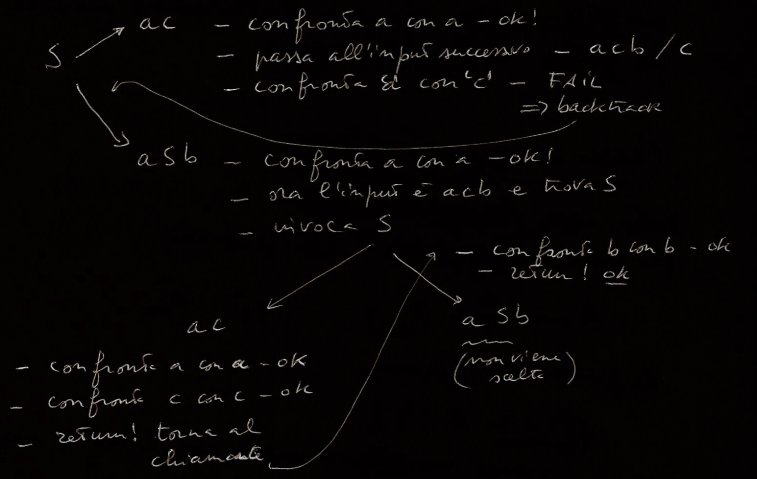
\includegraphics[width=10cm]{top-down_discesa_esempio.png}
    \end{center}

    \begin{center}
            \begin{tabular}{c c}
            \textbf{input} & \textbf{Stack delle chiamate} \\
            \\
            \underline{a} a c b & S \\
            \phantom{a}  & \underline{a} c \\
            \phantom{a} \underline{a} c b & c \textit{fail} \\
            \\
            \underline{a} a c b & S \\
            \phantom{a} & \underline{a} S b \\
            \phantom{a} \underline{a} c b & S b \\
            \phantom{a} & \underline{a} c b \\
            \phantom{a} \underline{c} b & \underline{c} b \\
            \underline{b} & b \\
            & \underline{ok} \\
            \end{tabular}
    \end{center}
}
Tuttavia il parser a discesa ricorsiva è \red{parecchio inefficiente a causa della sua natura nondeterminista}, vi è infatti la necessita nel peggiore dei casi di esplorare tutte le alternative

\teorema{
    Sia $w$ la lunghezza della stringa in inout, e sia $b$ il  massimo numero di produzioni per uno stesso nonterminale, allora la complessità computazionale di un parser a discesa riscorsiva nel caso peggiore è:
    \[
        O(b^{|w|})    
    \]
}

Per ovviare ovviare a questo problema di infecenza dobbiamo guidare la scelta della produzione per creare un parser top-down deterministico. Per farlo occorrono delle fuzioni ausiliarie

\section{Parser predittivo}
Il \textbf{parser predittivo} è un tipo parser deterministico (sotto alcune specifiche condizione che si vedranno più avanti), molto più efficiente in quanto non ha il backtracking, tuttavia per definirlo occorre prima definire delle funzioni ausiliarie
\subsection{First}
\dfn{First}{
    Data una grammatica libera $G \text{ e }\alpha\in(T\cup NT)^*$, di definisce \textbf{First($\alpha$)} come l'insieme dei terminali che possono stare in prima posizione in una stringa che si deriva da $\alpha$ 
    \begin{itemize}
        \item per $a \in T, a \in First(\alpha) \iff \alpha \implies^* a\beta \text{ per }\beta\in(T\cup NT)^*$
        \item inoltre $(\alpha \implies^*\epsilon)\implies \epsilon \in First(\alpha)$
    \end{itemize}
}
\osservazione{
    Sia la grammatica
    \[
        A \to \alpha_1 | \alpha_2       
        \]
        Se $First(\alpha_1)\cap First(\alpha_2) = \emptyset$ la scelta della produzione è deterministica
        }
Qui vi è riportato un esempietto:
\esempio{
    \[
        A\to aB|bC       
    \]
    Si ha che:
    \begin{array}{l}
        First(aB)= \{a\} \\
        First(bC) = \{b\} 
    \end{array}
    Pertanto abbiamo del determinismo con un solo carattere in lettura
}
\subsubsection{algoritmo per calcolare il first}
\begin{algorithm}[H]
    \SetAlgoNlRelativeSize{-1}
    \SetNlSty{textbf}{}{}
    \caption{First()}
    \KwIn{Una grammatica credo}
    \KwOut{bho}
    
        \For{$x\in T$}{
            $First(x)\gets \{x\}$\tcp*{un terminale è il primo elemento di se stesso}
        }
        \For{$X\in NT$}{
            $First(X)\gets \emptyset$\tcp*{per ogni x non terminale si inizializza il suo first a "0"}
        }
        \While{
            almeno un $First(X)$ può essere modificato in una iterazione\
        }{
            \ForEach{$x\to Y_1,\dots,Y_k$}{
                \ForEach{$i=1$\KwTo $k$}{
                    \tcp{se ciascuno di questi simboli $y_1,\dots,Y_{i-1}$ può derivare la stringa vuota $\epsilon$}
                    \If{$Y_1,\dots,Y_{i-1}\in N(G)$ }{
                        $First(X)\gets First(X)\cup (First(Y_i)\backslash\{\epsilon\})$\tcp*{allora è possibile aggiungere gli elementi di $FIRST(Y_i)$ a $FIRST(X)$ per la produzione y_1,\dots,y_k}
                    }
                    \tcp{Se invece uno dei simboli da $Y_1$ a $Y_{i-1}$ non è annullabile, si interrompe la ricerca per quella produzione, perché non possiamo "saltare" i simboli non annullabili per arrivare a Y_i}
                }
            }
        }
        \ForEach{
            $X\in N(G)$
        }{
            $First(X) = First(X)\cup\{\epsilon\}$\;
        }
\end{algorithm}

In generale per una stringa $\alpha$ si ha che:
\begin{itemize}
    \item Se \( \alpha = \varepsilon \), allora \( FIRST(\alpha) = \{\varepsilon\} \).
    \item Se \( \alpha = X \beta \) e \( X \notin N(G) \), allora \( FIRST(X \beta) = FIRST(X) \).
    \item Se \( \alpha = X \beta \) e \( X \in N(G) \), allora $FIRST(X \beta) = (FIRST(X) \setminus \{\varepsilon\}) \cup FIRST(\beta)$
\end{itemize}

In pratica se 
\[
    A\to \alpha_1 | \dots | \alpha_k    
\]
si ha che
\[
    First(A) = First (\alpha_1)\cup\dots\cup First(\alpha_k)   
\]

\esempio{
    Si ossrvi la seguente grammatica:
    \[
        \begin{array}{l}
            S\to Ab|c\\
            A\to aA|\epsilon
        \end{array}       
    \]

    \begin{align*}
        FIRST(S) &= FIRST(Ab) \cup FIRST(c) \\
                 &= (FIRST(A) \setminus \{\epsilon\}) \cup FIRST(b) \cup \{\epsilon\} \\
                 &= \{a\} \cup \{b\} \cup \{c\} = \{a, b, c\}
    \end{align*}
    
    \begin{align*}
        FIRST(A) &= FIRST(aA) \cup FIRST(\epsilon) \\
                 &= \{a\} \cup \{\epsilon\} = \{a, \epsilon\}
    \end{align*}
}
\subsection{Follow}
\dfn{Follow}{
    Data una grammatica libera \( G \) e \( A \in NT \), definiamo che \( Follow(A) \) è l'insieme dei terminali che possono comparire immediatamente a destra di \( A \) in una forma sentenziale.

    \begin{itemize}
        \item Per ogni \( a \in T \), \( a \in Follow(A) \) se \( S \Rightarrow^* \alpha A a \beta \) per qualche \( \alpha \) e \( \beta \in (T \cup NT)^* \).
        
        \item \( \$ \in Follow(A) \) se \( S \Rightarrow^* \alpha A \) (Poiché \( S \Rightarrow^* S \), allora \( \$ \in Follow(S) \) !)
    \end{itemize}
}
Riporto qui un esempio 
\esempio{
    \begin{align*}
        S &\rightarrow A b \mid c \\
        A &\rightarrow a A \mid \varepsilon
    \end{align*}
    
    \[
    Follow(S) = \{\$\} \quad Follow(A) = \{b\}
    \]
    
    \begin{itemize}
        \item \( S \Rightarrow^* S \)
        \item \( S \Rightarrow^* Ab \)
    \end{itemize}    
}
\subsubsection{algoritmo per calcolare il Follow}
\begin{algorithm}[H]
    \SetAlgoNlRelativeSize{-1}
    \SetNlSty{textbf}{}{}
    \caption{Follow()}
    \KwIn{Una grammatica credo}
    \KwOut{bho}
    
        \ForEach{$X\in NT$}{
            $First(X)\gets \emptyset$\tcp*{per ogni X non terminale si inizializza il suo first a "0"}
        }
        $Follow(S)\gets \{\$\}$\;
        \While{
            almeno un $Follow(X)$ può essere modificato in una iterazione
        }
        {
            \ForEach{$X\to\alpha Y\beta$}{
                $Follow(Y)\gets Follow(Y)\cup(First(\beta)\backslash \{\epsilon\})$\;
            }
            \ForEach{$X\to\alpha Y$}{
                \ForEach{$X\to \alpha \beta, \epsilon\in First(\beta)$}{
                    $Follow(Y)\gets Folloe
                    (Y)\cup Follow(X)$\;
                }
            }
        }
\end{algorithm}
in pratica, occorre cercare tutte le produzioni in cui $Y\in NT$ appare e, per ognuna di esse, applicare la 1 o la 2 sopra
\esempio{
    \begin{center}
        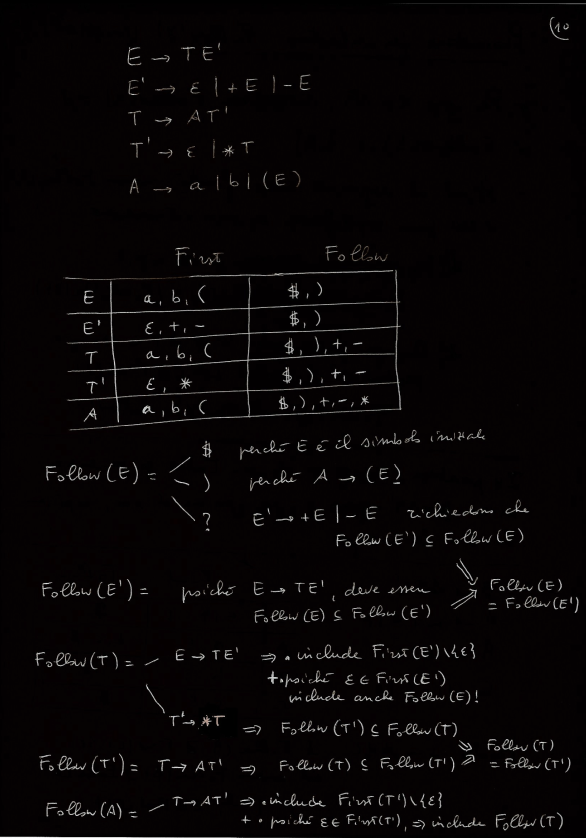
\includegraphics[width=10cm]{esempio_follow.png}
    \end{center}
}
Adesso che abbiamo introdotto i le procedure First e Follow occorre fare un passo in più per definire i parser

\subsection{Parser per linguaggi $LL(1)$}
\subsubsection{tabella di parsing LL(1)}
La tabella di parsing $LL(1)$ è una struttura di dati usata nei parser sintattici molto utili per risolvere il non determinismo. Questi parser leggono l'input da sinistra a destra (da qui il primo "L" di "LL"), costruendo una derivazione sinistra, o leftmost (da qui il secondo "L") e usano un solo simbolo di lookahead (da cui il "(1)").

Questa tabella è formata da una \textbf{matrice bidimensionale $M$} che è formata da:
\begin{itemize}
    \item \textbf{righe}: non-terminali
    \item \textbf{colonne}: terminali (incluso \$)
    \item \textbf{casella} $(A, a)$: $M[A, a]$ contiene le produzioni che possono essere scelte dal parser mentre tenta di espandere $A$ e l'input corrente è $a$.
\end{itemize}

Se ogni casella contiene \red{al più una produzione}, allora il parser è \red{deterministico}!


Per riempire la tabella occorre procedere in questo modo:

Per ogni produzione $A \rightarrow \alpha$:
\begin{enumerate}
    \item per ogni $a \in T$ e $a \in \text{First}(\alpha)$, inserisci $A \rightarrow \alpha$ nella casella $M[A, a]$
    \item se $\varepsilon \in \text{First}(\alpha)$, inserisci $A \rightarrow \alpha$ in tutte le caselle $M[A, x]$ per $x \in \text{Follow}(A)$ (x può essere \$)
\end{enumerate}

Ogni casella vuota, dopo aver elaborato tutte le produzioni, è un errore (cioè la funzione ricorsiva chiama `fail')

\subsubsection{grammatica $LL(1)$}

\dfn{grammatica $LL(1)$}{
    Una grammatica si definisce $LL(1)$ sse ogni casella della tabella di parsing $LL(1)$ contirne al più una produzione, ovvero non presenta conflitti
}

Si ha che \red{se $G=LL(1)$ allora il parser è predittivo e deterministico}, questo perché il parser ricostruisce l'albero di derivazione per l'input $w$, in modo top-down, predicendo quale produzione usare (tra le molte possibili) guardando il prossimo carattere dell'input

\teorema{
    $G$ è $LL(1)$ sse per ogni coppia di produzioni distinte con la stessa testa 
    \[
        A\to \alpha|\beta       
    \]
    si ha che \begin{enumerate}
        \item $First(\alpha)\cap First(\beta)=\emptyset$
        \item \begin{enumerate}
            \item $(\epsilon\in First(\alpha))\implies (First(\beta)\cap Follow(A) = \emptyset)$
            \item $(\epsilon\in First(\beta))\implies (First(\alpha)\cap Follow(A) = \emptyset)$
        \end{enumerate}
    \end{enumerate}
}
\dimostrazione{
    Se sono soddisfatte le condizione 1 e 2 per ogni coppia di produzioni distinte con medesima testa allora la tabella di parsing $LL(1)$ contiene al più una prodizone in ogni cassella. 
    Ma vale anche viceversa!
}

\subsubsection{Linguaggio $LL(1)$}
\dfn{Linguaggio $LL(1)$}{
    Un linguaggio si definisce $LL(1) \iff \exists G' \text{ grammatica } = LL(1)$ che lo genera 
}
\esempio{
    Sia $G$ la segunete grammatica:
    \[
        \begin{array}{l}
            S\to A|B\\
            A \to ab|cd\\
            B\to ad|cb
        \end{array}       
    \]
    Si può notare che $G$ non è $LL(1)$ dato che $S\to A|B$ e 
    \[
        \begin{array}{l}
            First(A) = \{a,c\}\\
            First(B) = \{a,c\}\\
            First(A)\cap First(B) = \{a,c\}
        \end{array}
    \]
    Dal teorema sopra fornito si può dimostrare che non è $LL(1)$\\
    Tuttavia si può manipolarla per farla diventare $LL(1)$, quindi espando $S$:
    \[
        S\to ab|cd|ad|cb    
    \]
    \[
        \begin{array}{l}
            S\to aT|cT'\\
            T\to b|d\\
            T'\to b|d
        \end{array}    
    \]
    Poi osservo che $T$ e $T'$ sono identici, sia quindi $G'$ la nuova grammatica:
    \[
        \begin{array}{l}
            S\to aT|cT  \\
            T\to b|d
        \end{array}
    \]
    Si può dimostrare che è $LL(1)$, pertanto, per la definizione di linguaggio $LL(1)$ e nonostante $G$ non sia $LL(1)$, si ha che $L(G) =\{ ab,cd,ad,cb\}$ è un linguaggio $LL(1)$ perché $G'$ che lo genera è una grammatica $LL(1)$  
    }

    \teorema{
        Ogni linguaggio regolare è generabile da una grammatica $G$ di classe $LL(1)$
    }
    \dimostrazione{
        Sia $L$ un linguaggio regolare, allora $\exists \text{ DFA }M=(Q,\Sigma , \delta, q_0, F):L=[M]$.

        A partira da $M$ si può costruire una grammatica regolare $G=(NT,T,S,R)$ basata sul seguente automa $M$:
        \begin{itemize}
            \item $NT=\{[q]|q\in Q\}$, cioè un non terminale per ogni stato $q$
            \item $T= \Sigma$ cioè un terminale per ogni simbolo dell'alfabeto
            \item $S=[q_0]$ simbolo iniziale lo stato iniziale
            \item $R$ (insieme delle produzioni) è definito come:
            \begin{itemize}
                \item se $\delta (q,a) = q'$, allora $[q]\to a[q']\in R$
                
                Infatti $\delta (q,a) = q'$ vuol dire che l'automa si trova allo stato $q$ e legge in input $a$ allora arriverà allo stato $q'$, che viene "tradotto" nella grammatica $[q]\to a[q']$ che corrisponde ad una produzione in cui il non terminale $[q]$ produce il terminale $a$ e il non terminale $[q']$, per passare al non terminale $[q']$ occorre, infatti, fare match con $a$
                \item se $q\in F$, allora $[q]\to \epsilon\in R$
            \end{itemize}
        \end{itemize}

        Poi che $M$ è deterministico, \( \forall q \in Q \forall a \in \Sigma \quad \exists! q'. q \xrightarrow{a} q' \), cioè \( [q] \) avrà una sola produzione \( [q] \to a[q'] \) che "inizia" per \( a \) e dato che se \( q \) è finale, allora \( [q] \to \epsilon \) è applicabile solo per i \(\text{Follow}([q]) = \{\$\} \implies \text{ nessun conflitto}\), dato che nessuna produzione genera $\$$, si ha che $G$ è $LL(1)$
    }
    \esempio{
        \begin{center}
            \begin{tikzpicture}[shorten >=1pt,node distance=2cm,on grid,auto] 
               \node[state,initial] (q_0)   {$q_0$}; 
               \node[state,accepting] (q_1) [right=of q_0] {$q_1$}; 
                \path[->] 
                (q_0) edge [loop above] node {a} ()
                      edge [bend left]  node {a} (q_1)
                (q_1) edge [bend left]  node {a} (q_0);
            \end{tikzpicture}
            \end{center}
            Le produzioni corrispondenti sono:
            \[
                \begin{array}{l}
                    [q_0] \to a[q_1]  a[q_0] \\
                    [q_1] \to a[q_0] \mid \epsilon
                    
                \end{array}
            \]
            
            La grammatica \( G \) è \( LL(1) \), perché:
            \[
                \text{First}(a[q_0]) \cap \text{First}(\epsilon) = \emptyset, \quad \text{First}(a[q_1]) \cap \text{First}(\epsilon) = \emptyset
            \]
    }
    
    Riporto qui un esempio di tabella di parsing $LL(1)$:
    \esempio{
        Sia $G$ la seguente grammatica:
        \[
            \begin{array}{l}
                E \to T E' \\
                E' \to \varepsilon \, | \, + T E' \, | \, - T E' \\
                T \to A T' \\
                T' \to \varepsilon \, | \, \ast T \\
                A \to a \, | \, b \, | \, (E)
                
            \end{array}       
    \]
    
    Si può costruire la seguente tabella di First e Follow:
    \[
        \begin{array}{|c|c|c|}
            \hline
            \text{Produzione} & \text{First} & \text{Follow} \\
            \hline
            E & a, b, ( & \$, ) \\
            E' & +, -, \varepsilon & \$, ) \\
            T & a, b, ( & +, -, \$, ) \\
            T' & \ast, \varepsilon & +, -, \$, ) \\
            A & a, b, ( & \ast, +, -, \$, ) \\
            \hline
        \end{array}
        \]
        
        Ed ecco a voi la tabella di parsing:
        \[
            \begin{array}{|c|c|c|c|c|c|c|}
                \hline
                & a & b & ( & + & \ast & \$ \\
                \hline
                E & E \to T E' & E \to T E' & E \to T E' &  &  &  \\
                E' &  &  &  & E' \to + T E' & E' \to - T E' & E' \to \varepsilon \\
                T & T \to A T' & T \to A T' & T \to A T' &  &  &  \\
                T' &  &  &  & T' \to \varepsilon & T' \to \ast T & T' \to \varepsilon \\
                A & A \to a & A \to b & A \to (E) &  &  &  \\
                \hline
            \end{array}
            \]
            
            \begin{center}
                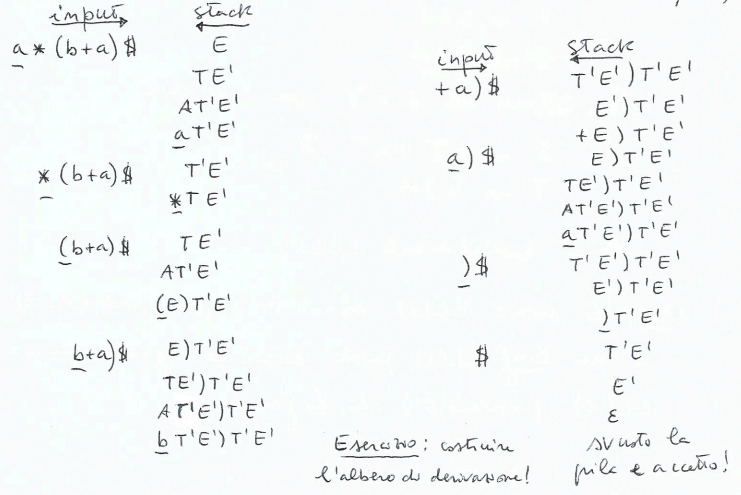
\includegraphics[width=7cm]{Parser_con_pila.png}
            \end{center}   
}

\subsubsection{Algoritmo Per il calcolo di un parser $LL(1)$}

\begin{algorithm}
    \caption{Parser $LL(1)$}
    \KwIn{Stringa $w$}
    \KwOut{Niente}

    $Pila\gets S\$$\tcp*{cima della pila a sinistra}
    $X\gets S$ \tcp*{top della pila}
    \tcp{lettura in input}
    $input \gets w\$$\;
    $i_c = \text{ primo carattere dell'input}$\;
    \tcp{viene eseguito il ciclo While finché la pila non è vuota o l'input non è stato consumato}
    \While{$X\neq \$$}{
        \If{$X$ è un terminale}{
            \tcp{si controlla se $X$ fa "match" con $i_c$}
            \If{$X = i_c$}{
                Pop $X$ dalla pila\tcp*{rimuovo $X$ dalla pila}
                avanza $i_c$ sull'input\;
            }
            \Else{
                Errore()\tcp*{no match}
            }
        }
        \Else{
            \tcp{se nella tabella di Parsing $M$ esiste una regola $X\to Y_1, \dots, Y_n$}
            \If{$M[X,i_c] = X\to Y_1, \dots, Y_n$}{
                Pop $X$ dalla pila\;
                Push $Y_1, \dots, Y_n$ sulla pila \tcp*{mette sulla pila i simboli $Y_1, \dots, Y_n$ con $Y_1$ in cima}
                In output la produzione $X\to Y_1, \dots, Y_n$\; 
            }
            \Else{
                Errore ()\tcp*{se non esiste una regola  in $M[X,i_c]$ si genera un errore, viene definito caso "bianco"} 
            }
            $X\gets$ top della pila\tcp*{Aggiorna $X$ con il nuovo simbolo in cima alla pila}
        }
    }
    \If{$i_c\neq \$$}{
        Errore()\tcp*{pila svuotata ma vi è ancora dell'input da leggere}
    }
\end{algorithm}



Un altro esempio:
\esempio{
    Sia $G$ la seguente grammatica:
    \[
    \begin{aligned}
        S &\to aAB \, | \, bS \\
        A &\to a \\
        B &\to b
    \end{aligned}
    \]
    Che genera il seguente linguaggio
    \[    
        L(G) = L\big(b^*aab\big)
    \]
    Si ha che questa grammatica \(G\) è LL(1), perché:
    \[
        First(aAB) \cap First(bS) = \varnothing, \quad \{a\} \cap \{b\} = \varnothing
    \]

    Si può prosegure con la tabella First e follow:
    \[
        \begin{array}{|c|c|c|}
        \hline
        Simbolo & First & Follow \\
        \hline
        S & a, b& \$ \\
        A & a& b \\
        B & b& \$ \\
        \hline
        \end{array}
    \]
    Da cui si può costruire la seguente tabella di parsing:
    \[
        \begin{array}{|c|c|c|c|}
        \hline
        & a & b & \$ \\
        \hline
        S & S \to aAB & S \to bS &  \\
        A & A \to a &  &  \\
        B &  & B \to b &  \\
        \hline
        \end{array}
    \]
    
    Viene qui descritto il funzionamento del parser con pila con diversi input:
    \begin{center}
        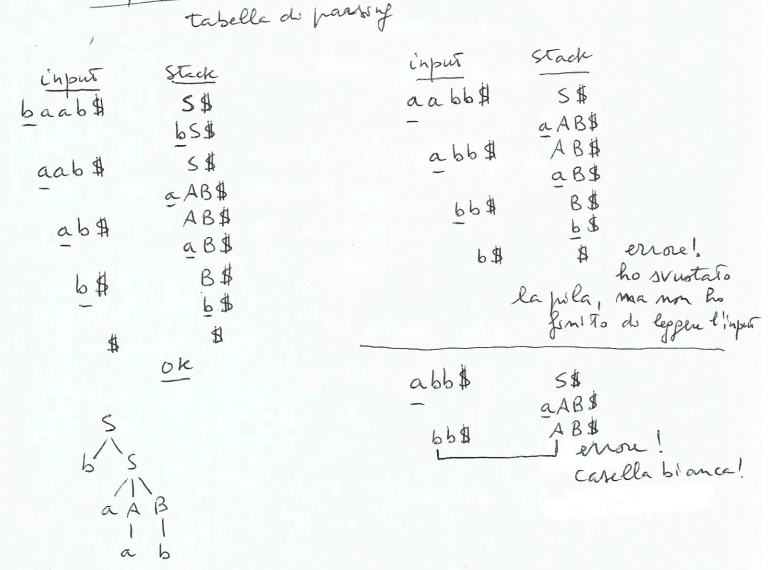
\includegraphics[width=10cm]{parser_pila_2.png}
    \end{center}


}

\subsection{Parser per linguaggi $LL(K)$}
\subsubsection{grammatiche $LL(K)$}
Le grammatiche $LL(k)$ sono "un'estensione" del concetto di grammatiche $LL(1)$, dove il parser ha la capacità di guardare in avanti fino a $k$ simboli per determinare le scelte di parsing

Per questi tipi di grammatica gli insiemi $First \text{ e }Follow$ assumo significati diversi rispetto a alle grammatiche $LL(K)$
\dfn{First $LL(K)$}{
    L'insieme \(First_k(\alpha)\) contiene tutte le stringhe di lunghezza \( k \) o minore derivabili dall'inizio di una produzione con \( \alpha \), in particolare
    $w\in First_k(\alpha) \iff \alpha \implies^{*}w\beta \text{ con } |w|=k,w\in T^{*}, \beta\in (T\cup NT)^* \text{ oppure }  \alpha \Rightarrow^* w  \text{ con } |w| \leq k \text{ e }  w \in T^* $
}
\dfn{Follow $LL(K)$}{
    L'insieme Follow\(_k(A)\) definisce quali stringhe possono apparire immediatamente dopo un simbolo non terminale \( A \) in una derivazione a partire dal simbolo iniziale \( S \). In particolare:
    \( w \in \text{Follow}_k(A) \) se \( S \Rightarrow^* \alpha A w \beta \) con \( |w| = k \), \( w \in T^* \), e \( \alpha, \beta \in (T \cup NT)^* \), oppure, \( S \Rightarrow^* \alpha A w \) con \( |w| \leq k \) e \( w \in T^* \).
}

\subsubsection{Tabella di Parsing $LL(K)$}
\begin{itemize}
    \item \textbf{Righe}: non terminali.
    \item \textbf{Colonne}: $\{ w \in T^* \mid |w| \leq k \}$ (solo quelle necessarie).
\end{itemize}

\noindent Per ogni produzione $A \to \alpha$, la tabella $M[A, w]$ contiene:
\begin{itemize}
    \item $A \to \alpha$, per ogni $w \in \text{First}_k(\alpha)$ ($w \neq \varepsilon$);
    \item $w \in \text{Follow}_k(A)$ se $\varepsilon \in \text{First}_k(\alpha)$.
\end{itemize}

\noindent Ogni entrata/casella contiene al più una produzione. Se non esistono $w_1$ e $w_2$ tali che $w_1$ prefisso di $w_2$ con le due entrate corrispondenti su una riga entrambe riempite, allora $G$ è una grammatica LL(k).

\vspace{1em}
\noindent \textbf{Nota Bene:} 
Le colonne sono tante quante sono le stringhe $w$ che appartengono a $\text{First}_k(\alpha)$ per $A \to \alpha$ o a $\text{Follow}_k(A)$ per $A \to \alpha$. Questo va verificato per tutte le produzioni:
\[
w \in \text{First}_k(\alpha).
\]

\esempio{
    Sia $G$ la seguente grammatica
    \[
        S\to aSb\mid ab\mid c
    \]
    Si ha che $L(G) = \{a^nb^n\mid n\geq 1\}\cup\{a^ncb^n\mid n\geq 0\}$, inoltre:
    \begin{itemize}
        \item $First_2(aSb) =\{aa,ac\}$
        \item $First_2(ab) =\{ab\}$
        \item $First_2(c) = \{c\}$
    \end{itemize}

    Si può dimostrare che $G$ è $LL(2)$ dato che:
    \begin{itemize}
        \item $First_2(aSb)\cap First_2(ab)=\varnothing$
        \item $First_2(aSb)\cap First_2(ab)=\varnothing$
        \item $First_2(aSb)\cap First_2(ab)=\varnothing$
    \end{itemize}
    Da cui si può ricavare la tabella di parsing:
    \[
        \begin{array}{|c|c|c|c|c|}
        \hline
        Simbolo & aa & ab & ac & c \\
        \hline
        S & S \to aSb& S\to ab&S\to aSb & S\to c
        \hline
        \end{array}
    \]

}
        
\teorema{
    \begin{itemize}
        \item Una grammatica ricorsiva sinistra non è $LL(K)$ per nessun $K$
        \item Una grammatica ambigua non è $LL(K)$
        \item Se $G$ è $LL(K)$ per qualche $k$, allora $G$ non è ambigua 
        \item Se $G$ è $LL(K)$, allora $L(G)$ è libero deterministico
        \item esiste $L$ libero deterministico tale che non esiste G di classe $LL(K)$ per nessun $K$, tale che $L=L(G)$
    \end{itemize}
}


Viene qui riportato il funzionamento del parser con pila:
\subsubsection{Linguaggio $LL(K)$}

\dfn{Linguaggio $LL(K)$}{
    un linguaggio $L$ è di classe $LL(K)$ se $G$ di classe $LL(K)$ tale che $L=L(G)$
}

\teorema{
    $\forall k\geq 0$, la classe dei linguaggi $LL(K)$ contiene strettamente la classe dei linguaggi $LL(K)$
}
\osservazione{
    $\forall k\geq 0,$ la classe dei linguaggi $LL(K+1)$ contiene strettamente la classe dei linguaggi $LL(K)$
    \begin{center}
        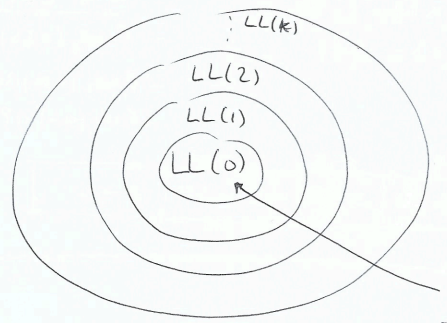
\includegraphics[width=10cm]{gerarchia_dei_linguaggi.png}
    \end{center}
    Si ha che: $(\forall A \in NT, \quad \exists! \alpha \in (T \cup NT)^*, \quad A \to \alpha \implies G \text{ è } LL(0))\implies L(G) = \{w\}$ ovvero una sola parola al massimo
}

\red{Nella pratica tuttavia si usano solo $LL(1)$}, spesso la si può manipolare trasformandola in $LL(1)$

\esempio{
    \[
        \begin{array}
            S\to Asb!ab!c\\
        \end{array}       
        
    \]
    $G$ è un $LL(2)$ ma non $LL(1)$
    Si fattorizza
    \begin{array}{l}
        S\to aT|c\\
        T\to Sb|b
    \end{array}
    Ottenuta fattorizzando $G$ è $LL(1)$ infatti:
    \begin{itemize}
        \item $First(aT)\cap First(c)=\varnothing$
        \item $First(Sb)\cap First(b)=\varnothing$
    \end{itemize}
    Si ha che $L = \{a^n b^n\mid n\geq 1\}\cup \{a^ncb^n\mid n\geq 0\}$ è un linguaggio di classe $LL(1)$ perché $G'$ è $LL(1)$
}
\subsubsection{Casi speciali}
Sia 
\[
    L= \{a^i b^j | i\geq j\} \text{ è libero deterministico}    
\]
Ma non è $LL(K)$ per nessun $K$!

Adesso, mostriamo una grammatica per $L$ e dimostriamo che non è LL(K) per nessun $K$.
Sia $G$ la seguente grammatica:
\[
    \begin{array}{l}
        S\to aS|B\\
        B\to aBb|\epsilon    
    \end{array}
\]

\begin{center}
    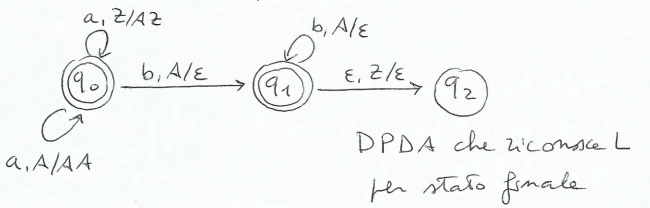
\includegraphics[width=10cm]{l_libero_deterministico_non_LL(K).png}
\end{center}

Sia $G$ una grammatica libero per $L$
\[
    S\to aS\mid B \\
    B\to aBb \mid \epsilon    
\]
e poniamo $L=L(G)$

%! NON HO CAPITO CAZZO

Per scegliere tra $S\to aS$ e $S\to B$ dovrei leggere fino in fondo l'input per sapere quante $b$ in meno di $a$ ci sono nella stringa! Allora $G$ non può essere $LL(k)$ per nessun $k$. Infatti quanto possa essere grande il $K$ posso trovare una stringa più lunga che richiede di leggere più di $k$ simboli di lookahead

Non è tuttavia possibile alcuna $G'$ e $k$ tali che
\[
    L(G') = L \text{ e }G'\in L(K)    
\]
La dimostrazione non verrà illustrata 

\end{document}
